\documentclass[11pt, a4paper]{scrartcl}
% Packages
\usepackage[margin=1.25in]{geometry}
\usepackage{index}
\usepackage{amsbsy} % Bold math symbols
\makeindex
\usepackage[utf8]{inputenc}
\usepackage{tcolorbox}
\usepackage[T1]{fontenc}
\usepackage{varwidth}
\usepackage{textcomp}
\usepackage{mathrsfs}
\usepackage{amsmath, amssymb}
\usepackage{esint}
\usepackage{titlesec}
\usepackage{xcolor}
\usepackage{titling}
\usepackage{braket}
\usepackage[linktocpage]{hyperref}
\usepackage{multicol}
\setlength{\columnsep}{2em}
\usepackage{caption}
\usepackage{amsthm}
\usepackage{import}
\usepackage{cancel}
\usepackage{caption}
\usepackage{nicematrix}
\usepackage{mathtools}
\usepackage{enumerate}
\usepackage{graphicx}
\usepackage{tikz}
\usetikzlibrary{arrows.meta,decorations.pathreplacing}
\usetikzlibrary{decorations.markings}

\tikzset{
    flow/.style={
        postaction={
            decorate,
            decoration={
                markings,
                mark=at position 0.55 with {\arrow{>}}
            }
        }
    }
}
\usepackage{pgfplots}
\pgfplotsset{compat=1.18}
\usepackage[italian]{babel}
% To reset footnote numbering each page
\usepackage[perpage]{footmisc}
\usepackage{setspace}
\setstretch{1.2}

% Titles 
\title{Note di Fisica statistica}
\author{}
\date{}


% svolgimento
\newenvironment{svolgimento}{\renewcommand\qedsymbol{$\blacksquare$}\begin{proof}[Svolgimento]}{\end{proof}}

\newtheoremstyle{style}% name of the style to be used
{5pt}% measure of space to leave above the theorem. E.g.: 3pt
{5pt}% measure of space to leave below the theorem. E.g.: 3pt
{\normalfont}% name of font to use in the body of the theorem
%{15pt}% measure of space to indent
{0pt}% measure of space to indent
{\noindent\bfseries}% name of head font
{}% punctuation between head and body
{ }% space after theorem head; " " = normal interword space
{\thmname{#1}\thmnumber{ #2}{\thmnote{ (#3)}.\ }}


\theoremstyle{style}
\newtheorem{esempio}{Esempio}[section]
\newtheorem{definizione}{Definizione}[section]
\newtheorem{prop}{Proposizione}[section]
\newtheorem{teorema}{Teorema}[section]
\newtheorem{lemma}{Lemma}[teorema]
\newtheorem{corollario}{Corollario}[teorema]
\newtheorem{osservazione}{Osservazione}[section]
\newtheorem{notazione}{Notazione}[section]

\newtheoremstyle{style1}% name of the style to be used
{5pt}% measure of space to leave above the theorem. E.g.: 3pt
{5pt}% measure of space to leave below the theorem. E.g.: 3pt
{\normalfont}% name of font to use in the body of the theorem
%{15pt}% measure of space to indent
{0pt}% measure of space to indent
{\noindent\bfseries\color{red}}% name of head font
{}% punctuation between head and body
{ }% space after theorem head; " " = normal interword space
{\thmname{#1}\thmnumber{ #2}{\thmnote{ (#3)}.\ }}

\theoremstyle{style1}
\newtheorem{esercizio}{Esercizio}[section]


%% Generic box
\newtcolorbox{eqbox}[1][]
{
colback=gray!10,
arc=0pt,
boxrule=0pt,
title=#1
}

 \newenvironment{boxenv}[1][]{
    \begin{eqbox}[#1]
    }{
   \end{eqbox}
}



%%%%%%%%%% Medie con integrali multipli
\def\Yint#1{\mathchoice
    {\YYint\displaystyle\textstyle{#1}}%
    {\YYint\textstyle\scriptstyle{#1}}%
    {\YYint\scriptstyle\scriptscriptstyle{#1}}%
    {\YYint\scriptscriptstyle\scriptscriptstyle{#1}}%
      \!\iint}
\def\YYint#1#2#3{{\setbox0=\hbox{$#1{#2#3}{\iint}$}
    \vcenter{\hbox{$#2#3$}}\kern-.51\wd0}}
\def\longdash{{-}\mkern-3.5mu{-}} 
   % consider using "\mkern-7.5mu" if esint package is loaded
\def\tiltlongdash{\rotatebox[origin=c]{15}{$\longdash$}}
\def\fiint{\Yint\tiltlongdash}

\def\Zint#1{\mathchoice
    {\YYint\displaystyle\textstyle{#1}}%
    {\YYint\textstyle\scriptstyle{#1}}%
    {\YYint\scriptstyle\scriptscriptstyle{#1}}%
    {\YYint\scriptscriptstyle\scriptscriptstyle{#1}}%
      \!\iiint}
      \def\tilongdash{\mkern6mu{-}\mkern-4mu{-}\mkern-5mu{-}} 
   % consider using "\mkern-7.5mu" if esint package is loaded
\def\titiltlongdash{\rotatebox[origin=c]{15}{$\tilongdash$}}
\def\fiiint{\Zint\titiltlongdash}

%Captions
\captionsetup[figure]{font=footnotesize,labelfont=footnotesize}
\captionsetup[table]{font=footnotesize,labelfont=footnotesize}
%Titlesec
\titleformat{\section}
{\fontsize{15}{20}\sffamily\scshape}
{\normalfont\color{gray}{\fontsize{20}{20}\selectfont\thesection}}
{0.7em}
{}
\hypersetup{colorlinks,breaklinks, linkcolor=[RGB]{74, 122, 164}}
\definecolor{asdf}{HTML}{4a7aa4}
% Personalizza la formattazione della subsection
\titleformat{\subsection}[block]{\fontsize{13}{20}\bfseries}{\normalfont\thesubsection}{.5em}{}


% Personalizza la formattazione della subsubsection
\titleformat{\subsubsection}[block]{\fontsize{12}{20}\bfseries}{\normalfont\thesubsubsection}{.5em}{}

% Maketitle customization
\renewcommand{\maketitle}{
\begin{center}
{\sffamily
{\fontsize{20}{20}\selectfont\MakeUppercase\thetitle}}

\vspace{0.2in}

{\large\scshape\sffamily\theauthor}
\end{center}
}

%Evaluate symbol
\DeclareMathOperator{\di}{d\!}
\newcommand*\Eval[3]{\left.#1\right\rvert_{#2}^{#3}}

%%%%%%% Numero delle equazioni in formato a.b
\numberwithin{equation}{subsection}
%%%%%

%%%%%%%%%% Personalizzazione numeri lista
\renewcommand{\theenumi}{(\arabic{enumi})}

%%%% Table of contents

\usepackage[titles]{tocloft}

\renewcommand{\cftdot}{}
\usepackage{titletoc}
%\setcounter{tocdepth}{2}

%%%%%%%%%%%%%%%% Toc style

% Personalizzazione scritta indice


% Font
\usepackage[osf]{newpxtext}
\usepackage{sansiwona}
\begin{document}
\maketitle
\newpage
\tableofcontents 
\newpage
\section{Introduzione alla meccanica statistica}
\subsection{Principi della meccanica statistica}

Per $\mathcal{N}$ copie dello stesso sistema, se il microstato $i$-esimo si estrae $\mathcal{N} _i$ volte, la probabilit\`a che venga estratto \`e data da 
\[
p_i = \frac{\mathcal{N} _i}{\mathcal{N} }
\] 
Il fatto che i microstati si contino con indice discreto \`e dato dal fatto che occupano una porzione di un certo volume nello spazio delle fasi.
I principi sono i seguenti.
\begin{enumerate}[(a).]
	\item \textbf{Principio di equiprobabilit\`a.} Cellette di uguale volume nello spazio delle fasi hanno, a priori, la stessa probabilit\`a di essere estratte.
	\item \textbf{Ammissibilit\`a delle estrazioni.} Gli stati in cui il sistema si pu\`o trovare devono rispettare certe condizioni legate a variabili macroscopiche, che definiscono l'ensemble con cui si descrive il sistema.
		\begin{itemize}
			\item \textit{Ensemble microcanonico:} sono costanti $N$, $V$ e $E$ (energia totale), quindi sono accessibili solo i microstati con energia fissa pari a $E$.
			\item \textit{Ensemble canonico:} sono costanti $N$, $V$ e $T$ (sistema a contatto con bagno termico) ed \`e nota l'energia interna del sistema:
				\[
				U = \langle E \rangle = \frac{1}{\mathcal{N} } \sum_{i}^{} \mathcal{N} _i E_i = \sum_{i}^{} p_i E_i 
				\] 
			\item \textit{Ensemble gran canonico:} sono costanti $T$, $V$ e $\mu $, in quanto il sistema scambia energia e particelle con l'ambiente, a temperatura e potenziale chimico costanti.
		\end{itemize}
	\item Per $\mathcal{N} \to +\infty$, si considera solo la distribuzione pi\`u probabile, mentre le altre sono trascurabili.
\end{enumerate}
Ora si stabilisce come si calcola la probabilit\`a di una distribuzione.
Si indica con la successione $\left\{ i_k \right\} _{k=1} ^\mathcal{N} $ una successione di indici, dove $i_k$ rappresenta il microstato in cui si trova la copia $k$-esima del sistema.
Visto che ogni sequenza \`e equiprobabile, la probabilit\`a di una deve essere proporzionale alla sua molteplicit\`a $\mathcal{M} $, cio\`e al numero di sequenze distinte di estrazioni che portano ad una identica distribuzione\footnote{Per esempio, se $\mathcal{N}=3$, con due uscite nel microstato $1$ e una uscita nel microstato $2$ (cio\`e $N_1=2$ e $N_2=1$), si ha le sequenze $i_k$ che portano alla stessa distribuzione sono $(1,1,2)$, $(1,2,1)$, $(2,1,1)$.}.
Allora, la distribuzione pi\`u probabile sar\`a quella con $\mathcal{M} $ pi\`u alto.

Per determinare la molteplicit\`a, si considera che permutare due indici relativi allo stesso microstato lascia invariata la successione\footnote{Ad esempio $({\color{red}1},{\color{blue}1},2)=({\color{blue}1},{\color{red}1},2)$.}, quindi 
\[
\mathcal{M} (\mathcal{N} _1,\mathcal{N} _2,\ldots) = \frac{\mathcal{N} !}{\mathcal{N} _1! \mathcal{N} _2! \cdots} = \frac{\mathcal{N} !}{\prod_i \mathcal{N} _i!}
\] 
Per $\mathcal{N} \to +\infty$, si pu\`o usare la formula di Stirling:
\[
\log \mathcal{N} ! \simeq \mathcal{N} \big(\log\mathcal{N} -1\big) 
\] 
da cui
\[
\begin{split}
	\log\mathcal{M} &\simeq \mathcal{N} (\log\mathcal{N} -1) - \sum_{i}^{} \mathcal{N} _i ( \log\mathcal{N} _i - 1) = \mathcal{N} \log\mathcal{N}- \sum_{i}^{} \mathcal{N} _i \log\mathcal{N} _i\\
			&= \mathcal{N} \log\mathcal{N} -\mathcal{N} \sum_{i}^{} p_i(\log p_i + \log\mathcal{N} ) = - \mathcal{N} \sum_{i}^{} p_i \log p_i
\end{split}
\] 
dove si \`e usato che $\sum_{i}^{} \mathcal{N} _i = \mathcal{N} $, $\mathcal{N} _i = \mathcal{N} p_i$ e $\sum_{i}^{} p_i = 1$.
Visto che si deve massimizzare $\mathcal{M} $, la costante $\mathcal{N} $ \`e ininfluente, quindi si considera 
\begin{equation}
	\log\mathcal{M} \simeq - \sum_{i}^{} p_i \log p_i
\end{equation}
L'entropia, in meccanica statistica, si definisce come
\begin{equation}
	S = -\kappa _B \sum_{i}^{} p_i \log p_i
\end{equation}
Il logaritmo serve a renderla estensiva, mentre $\mathcal{M} $, in un certo senso, misura l'ignoranza sul sistema.
Questo motiva $S \propto \log\mathcal{M} $; la costante di proporzionalit\`a si pu\`o dimostrare essere proprio $\kappa _B$.

\subsection{Ensemble canonico}
Si ammette la possibilit\`a che il sistema scambi energia con l'ambiente, il quale funge da bagno termico e mantiene $T$ costante.
Si assume, inoltre, che $N_B \gg N_S$ (il bagno ha molte pi\`u particelle del sistema), ma comunque entrambi rilevanti a livello macroscopico.

Si tratta l'universo con il formalismo microcanonico, visto che la sua energia \`e costante; allora
\[
E < E_S + E_B < E+ \Delta E
\] 
con $E$ energia universo e $\Delta E$ incertezza associata.
Per avere una buona definizione di bagno termico, deve anche valere $E_B \gg E_S$.
Visto che $E_B$ ed $E_S$ sono vincolate dall'energia $E$ dell'universo, si pu\`o assumere che la distribuzione del sistema sia 
\[
\rho _S \left(\left\{ \vec{q}_S \right\} , \left\{ \vec{p}_S \right\} \right) \sim \Gamma_B(E_B)
\] 
con $\Gamma(E_B)$ numero di microstati del bagno a energia $E_B$.
Per il terzo principio della meccanica statistica, ci si limita a considerare il valore $\overline{E}_B$ che massimizza $\Gamma_B$, con altri trascurabili; allora
\[
	S_B(E_B) = \kappa _B \log\Gamma_B(E_B) \simeq S_B(E) - E_S\Eval{\frac{\partial S_B}{\partial E_B} }{E_B=E}{}+\ldots
\] 
ottenuto sviluppando ad $E$.
Usando che $\frac{1}{T}=\Eval{\frac{\partial S}{\partial E} }{V}{}$, si ha $S_B(E_B) \simeq S_B(E) - E_S / T$, da cui 
\[
\Gamma_B(E_B) = \Gamma_B(E-E_S) \simeq e^{\frac{1}{\kappa _B} S_B(E)}e^{-\frac{E_S}{\kappa _BT}}
\] 
da cui $\rho _S \sim e^{-E_S / (\kappa _B T)}$.





























\newpage
\section{Meccanica statistica classica dei sistemi interagenti}
\subsection{Sistemi interagenti}
Si considera un gas di $N$ particelle descritto da un'hamiltoniana 
\[
H = \sum_{j=1}^{N} \frac{p_j^2}{2m} + \mathcal{V} (\vec{x}_1,\ldots,\vec{x}_N)
\] 
dove $\mathcal{V}$ \`e il termine di interazione, che si assume indipendente dai momenti.
Si descrive tale sistema con il formalismo canonico; allora
\[
Z = \frac{1}{N! h^{3N}} \int d^N \vec{q} d^N \vec{p} \ e^{- \beta  H} 
\] 
L'integrale nei momenti \`e facile perch\'e risulta essere un integrale gaussiano\footnote{Si ricorda che $\int_{-\infty} ^{+\infty} e^{-\alpha x^2} \ dx = \sqrt{\pi / \alpha } $.}:
\[
\frac{1}{h^{3N} } \int d^N \vec{p} \ e^{-\beta  \sum_{j}^{} \frac{p^2_i}{2m}}  = \left(\frac{2\pi m }{h^2 \beta }\right) ^{3N / 2} 
\] 
La parte complicata \`e relativa a quella sulle posizioni. 
Si indica con $Z_N$ la parte della funzione di partizione relativa all'integrale della parte interagente dell'hamiltoniana:
\[
Z_N := \int d^N \vec{x} \ e^{-\beta  \mathcal{V} (\vec{x}_1,\ldots,\vec{x}_N)} 
\] 
Conoscendo $Z_N$, si ricava tutta la fisica del sistema. 
Infatti:
\[
\begin{split}
	&F= -\frac{1}{\beta }\log \left[\frac{1}{N!}\left(\frac{2\pi m }{h^2 \beta }\right)^{3N / 2}  \right]  - \frac{1}{\beta }\log Z_N\\
	& U = - \frac{\partial }{\partial \beta } \log Z = \frac{3}{2} N \kappa _B T + \kappa _B T^2 \Eval{\frac{\partial }{\partial T} \log Z_N}{T}{}\\
	& p = \Eval{- \frac{\partial F}{\partial V}}{T}{} = \kappa _B T \Eval{\frac{\partial }{\partial V} \log Z_N}{T}{}
\end{split}
\] 
da cui si ricava l'equazione di stato 
\begin{equation}\label{1-steq}
	\frac{pV}{N\kappa _B T} = \frac{V}{N} \Eval{\frac{\partial }{\partial V} \log Z_N}{T}{}
\end{equation}
\begin{osservazione}
Nel limite non interagente in cui $\mathcal{V} \equiv 0$, si vede che $Z_N = V^N$ (volume nel quale \`e confinato il gas), per cui
\[
\frac{pV}{N\kappa _B T} = \frac{V}{N}N \frac{1}{V}= 1 \implies pV = N \kappa _B T
\] 
che \`e l'equazione di stato del gas perfetto.
\end{osservazione}
\subsubsection{Interazione a due corpi}
Si studia il caso in cui il potenziale sia della forma 
\[
\mathcal{V} (\vec{x}_1,\ldots,\vec{x}_N) = \sum_{i<j}^{} v (\vec{x}_i - \vec{x}_j)
\] 
La tecnica per calcolare $Z_N$ \`e procedere iterativamente: si cerca di trovare $Z_{N+1} $ in termini di $Z_N$, assumendo quest'ultima nota.
Di seguito, si svolgono passaggi per esplicitare $Z_N$ nel caso in cui si abbiano $N+1$ particelle.
\[
\begin{split}
	Z_{N+1} &= \int d^N \vec{x} \int d \vec{x}' \ e^{-\beta \sum_{i<j}^{} v(\vec{x}_i -\vec{x}_j)}  e^{-\beta \sum_{j=1}^{N} v(\vec{x}' - \vec{x}_j)} \\
		&= \frac{\displaystyle \int d^N \vec{x} \int d\vec{x}'\ e^{-\beta \sum_{i<j}^{} v(\vec{x}_i -\vec{x}_j)} e^{-\beta \sum_{j}^{} v(\vec{x}' -\vec{x}_j)}  }{\displaystyle \int d^N \vec{x} \ e^{-\beta \sum_{i<j}^{} v(\vec{x}_i-\vec{x}_j)} } \int d^N \vec{x} \ e^{-\beta \sum_{i<j}^{} v(\vec{x}_i - \vec{x}_j)} \\
		& = \left\langle \int d\vec{x}' \ e^{-\beta \sum_{j}^{} v(\vec{x}' - \vec{x}_j)}  \right\rangle_N Z_N
\end{split}
\] 
dove il pedice $N$ alla media si riferisce al fatto che \`e pesata con la funzione di distribuzione per il sistema di $N$ particelle.

Per proseguire nello studio del sistema, si fa la seguente assunzione: \textit{l'interazione tra le particelle del sistema avviene esclusivamente a coppie}. 
Questo significa che, qualora due particelle si trovino vicine a tal punto da interagire, è estremamente improbabile che ve ne siano altre che interagiscono.	
Se le particelle $i$ e $j$ sono vicine, si scrive che $\vec{x}_i \sim \vec{x}_j$.
\begin{osservazione}
	Se $\vec{x}' \not \sim \vec{x}_i, \ \forall i=1,\ldots, N$, allora $e ^{- \beta \sum_{j}^{} v(\vec{x}' - \vec{x}_j)} \simeq 1$, per cui $Z_{N+1} \simeq VZ_N$.
\end{osservazione}
\noindent Trascurando il caso banale nell'osservazione, rimane da studiare il caso $\vec{x}' \sim \vec{x}_i$, per qualche $i=1,\ldots,N$.
In questo caso, si pu\`o considerare $e^{-\beta  \sum_{i<j}^{} v (\vec{x}_i - \vec{x}_j)} \simeq 1$, da cui
\[
Z_{N+1}  \simeq \frac{\displaystyle \int d \vec{x}' \int d ^N \vec{x}\ e^{-\beta  \sum_{i}^{} v(\vec{x}' - \vec{x}_i)} }{V^N} Z_N
\] 
Visto che le particelle sono indistinguibili
\[
Z_{N+1} \simeq \int d\vec{x}' \left(\int d\vec{y} \ e ^{-\beta v(\vec{x}' -\vec{y})}\right) ^N \frac{1}{V^N}Z_N
\] 
Aggiungendo e sottraendo $1$, l'integrale tra parentesi \`e
\[
\left[ V - \int d\vec{y} \left(1 - e^{-\beta  v(\vec{x}' - \vec{y})}\right)  \right] ^N
\] 
Ora si assume che il potenziale sia uniforme e, quindi, che $v(\vec{x}_i - \vec{x}_j) \equiv v(\lvert \vec{x}_{i} -\vec{x}_j  \rvert )$; tramite un cambio di coordinate, allora:
\[
\begin{split}
	&a:= \int dr \ 4 \pi r^2 \left(1-e^{-\beta v(r)}\right) \\
	&\Rightarrow Z_{N+1} \simeq \frac{1}{V^N} \left(\int d\vec{x}' (V-a)^N\right) Z_N = \frac{V (V-a)^N}{V^N}Z_N = V \left(1-\frac{a}{V}\right) ^N Z_N
\end{split}
\] 
visto che $(V-a)^N$ non dipende da $\vec{x}'$.
Allora, si vede che $Z_1 = V$, $Z_2 = V(1-a / V)Z_1$, e cos\`i via, per cui 
\[
Z_N = V^N \left(1- \frac{a}{V}\right) ^{1 + 2 + \ldots + (N-1)} = V^N \left(1- \frac{a}{V}\right) ^{\frac{N(N-1)}{2}} 
\] 
Infine, si osserva che, nel limite termodinamico, cio\`e per grandi $N,V$ e $N / V$ costante, si ha
\[
\left(1-\frac{a}{V}\right) ^{\frac{N(N-1)}{2}} = \exp \left[ \frac{N(N-1)}{2}\log\left(1-\frac{a}{V}\right)  \right] \simeq \exp \left[ \frac{N^2}{2} \log\left(1-\frac{a}{V}\right)  \right] \simeq \exp\left(\frac{-aN^2}{2V}\right)  
\] 
da cui
\[
Z_N \simeq V^N e ^{- aN^2 / (2V)} 
\] 
Questa \`e l'espressione di \textit{campo medio}. 

\subsubsection{Equazione di van der Waals}



Ora si riprende l'equazione di stato in \ref{1-steq}. 
Inserendo quanto appena ottenuto, si trova 
\[
\frac{pV}{N\kappa _B T} = 1 + \frac{Na}{2V}
\] 
Per capire meglio l'espressione, si esplicita $a$:
\[
\begin{split}
	a &= 4 \pi \int_{0} ^{+\infty} dr \ r^2 \left(1 - e ^{-\beta v(r)}\right) \\
	  &\simeq 4\pi \int_{0} ^b dr \ r^2 (1-0) + 4 \pi \int_{b} ^{+\infty} dr \ r ^2 \left(1-e^{-\beta  v}\right) \\
	  &\simeq \frac{4}{3}\pi b^3 - \frac{1}{\kappa _B T}4 \pi \int_{b} ^{+\infty} dr \ r^2 \big(-v(r)\big) \\
	  &= V_b - \frac{D}{T}
\end{split}
\] 
dove $V_b = \frac{4}{3}\pi b^3$ (volume sfera di raggio $b$) e $D = -\frac{1}{\kappa _B}\int_{b} ^{+\infty} dr \ 4\pi r^2 v(r)$.
Nella prima approssimazione sopra, si \`e scelto $v(r)$ simile a Lennard-Jones, approssimandolo come\footnote{Cio\`e a meno di un tratto di discesa, diventa subito negativo dopo $b$ e, dopo un minimo, si attesta sullo zero.}
\[
v(r) = \begin{cases}
	+\infty&\, r \in [0,b]\\
	       v(r)<0&\, r \in (b,+\infty)
\end{cases}
\] 
Nella seconda approssimazione, invece, si \`e assunto che $\lvert \beta v(r) \rvert \ll 1$, corrispondente a potenziale debole rispetto a $\kappa _B T$, per sviluppare l'esponenziale al primo ordine.
In questo modo, l'equazione di stato diventa 
\[
\frac{pV}{N\kappa _BT}\simeq 1+\frac{N}{2} \frac{V_b}{V}-\frac{ND}{2VT}
\] 
Questo pu\`o essere riscritto in una forma pi\`u nota:
\begin{equation}
	\left(p+\frac{a_w}{V^2}\right) \left(V-b_w\right) = N\kappa _B T
\end{equation}
dove $b_w = \frac{N}{2}V_b$ e $a_w = \frac{1}{2}N^2 \kappa _B D	$.
Questa \`e l'\textit{equazione di stato di van der Waals} (da cui i pedici $w$ in $a_w$ e $b_w$).
Questa equazione permette di dire che, sotto le ipotesi trattate, in particolare quella di gas diluito, il gas si pu\`o descrivere tramite l'equazione di stato del gas perfetto, a patto di correggere pressione e volume opportunamente:
\begin{itemize}
	\item il volume deve essere corretto perch\'e le particelle non sono puntiformi, ma occupano un volume (sono circa sfere), quindi non possono sovrapporsi (viene diminuito tramite $b_w$);
	\item la pressione viene aumentata per via del potenziale considerato, il quale include una coda attrattiva che tende a non far allontanare liberamente le particelle tra loro.
\end{itemize}
Ora se ne studiano le isoterme nel piano $(V,p)$. 
Si vede che, al variare del valore fisso di temperatura, se ne trova uno in particolare che definisce la curva risultante; questo si chiama \textit{temperatura critica}, $T_c$.
\begin{figure}[h!]
	\centering
	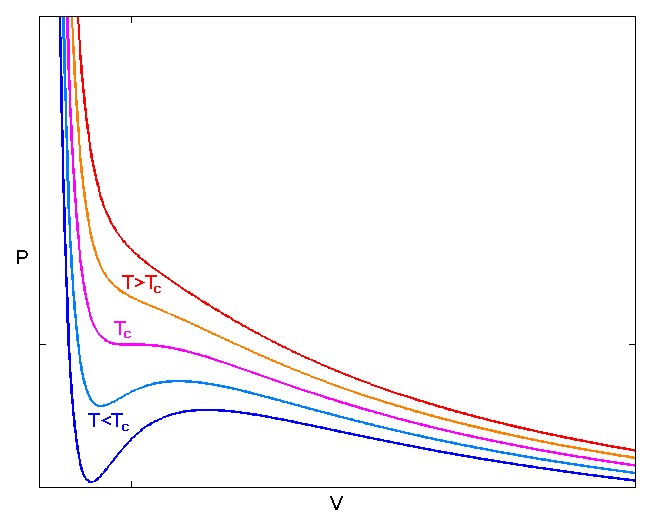
\includegraphics[width=.5\columnwidth]{vdw.png}
\end{figure}
Per $T>T_c$, la curva risultante assegna sempre una pressione ad un volume; nel caso di $T<T_c$, invece, la curva non \`e pi\`u iniettiva: si trovano dei valori di pressione raggiunti da volumi diversi.
Mentre nel caso $T>T_c$, la relazione $\Eval{\frac{\partial p}{\partial V} }{T}{}<0$ \`e sempre verificata, si vede che per $T<T_c$, la variazione di pressione al variare del volume pu\`o diventare positiva, il che rappresenta un problema fisico perch\'e indica instabilit\`a nel gas.
Quando $T=T_c$, invece, l'equazione diventa $(V-V_c)^3= 0$ e presenta un punto di flesso in $(T_c,p_c,V_c)$, dove 
\begin{equation}
	T_c = \frac{8}{27} \frac{a}{b}\frac{1}{N\kappa _B} \hspace{1cm} p_c = \frac{a}{27b^2}\hspace{1cm}V_c = 3b
\end{equation}
Si vedr\`a che questo punto, chiamato \textit{punto critico}, \`e relativo ad una transizione di fase del secondo ordine; i tre punti di volume corrispondenti ad un certo valore di pressione nel caso di $T<T_c$, una volta corretti, si vedranno corrispondere ad una transizione di fase del primo ordine. 
\begin{osservazione}
Definendo $\overline{p}= p / p_c$, $\overline{V} = V / V_c$ e $\overline{T} = T / T_c$, attorno al punto critico, l'equazione di van der Waals si pu\`o scrivere come
\[
\left(\overline{p} + \frac{3}{\overline{V}^2}\right) \left(\overline{V}-\frac{1}{3}\right) = \frac{8}{3}\overline{T}
\] 
nota come \textit{legge degli stati corrispondenti}.
Si nota che questa non contiene alcuna informazione sulla natura del gas in esame, ossia sulla sostanza di cui \`e composto, visto che si riescono a eliminare le variabili $a$ e $b$ da cui tale dipendenza deriva.
\end{osservazione}
\subsubsection{Costruzione di Maxwell}
\begin{center}
	\begin{minipage}
		{.45\columnwidth}
		Per risolvere il problema della zona instabile nel caso $T<T_c$, Maxwell ha proposto il seguente argomento.
		Il problema risiede nel fatto che, passando al grafico $(V,F)$ tramite $F = \int p \ dV$ a $T$ fissata, si vede che la curva prevista da van der Waals non minimizza l'energia libera di Helmholtz, causa dell'instabilit\`a.

		Allora si deve sostituire la parte prevista da van der Waals con una retta orizzontale a pressione $p_1=p_2$ che, nel grafico $(V,F)$, sia la tangente alla curva nei punti $V_1$ e $V_2$.
	\end{minipage}
	\hfill
	\begin{minipage}
		{.45\columnwidth}
	\centering
	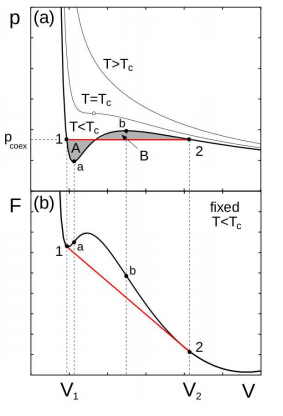
\includegraphics[width=.8\columnwidth]{max-constr-vdw.png}
	\end{minipage}
\end{center}
Questo permette di identificare i punti $1$ e $2$.
Le condizioni imposte da questo ragionamento sono:
\[
\begin{split}
	&p_1=p_2\implies \Eval{\frac{\partial F}{\partial V_1} }{T}{} =\Eval{\frac{\partial F}{\partial V_2} }{T}{}\\
	& \frac{F_2-F_1}{V_2-V_1}= \Eval{\frac{\partial F}{\partial V_1} }{T}{}
\end{split}
\] 
da cui
\[
 -\Eval{\frac{\partial F}{\partial V_1} }{T}{} (V_2-V_1) = -(F_2-F_1) \implies p_1 (V_2-V_1) = \int_{V_1} ^{V_2} p \ dV
\] 
Questo permette di concludere anche che la retta orizzontale $p_1=p_2$ nel grafico $(V,p)$ \`e tale per cui le aree $A$ e $B$ sono uguali.
Infine, si nota che, durante l'intera retta rossa individuata da Maxwell, la sostanza che compone il sistema coesiste allo stato liquido e gassoso: per $V\le V_1$, la sostanza \`e allo stato liquido; per $V\ge V_2$, la sostanza \`e allo stato gassoso; per $V \in (V_1,V_2)$, i due stati coesistono e la pressione \`e costante.

\subsection{Espansioni in clusters}
Si tratta di sviluppi di natura perturbativa, fondati sull'assunzione di gas con densit\`a \textit{piccola}.
Permette una descrizione pi\`u accurata e generale di un sistema composto da un gas reale; si ritrover\`a il caso di van der Waals come sviluppo al primo ordine non-banale.
\begin{osservazione}
Questi sviluppi sono adeguati quando il sistema non si trova vicino a transizioni di fase, le quali sono caratterizzate da non-analiticit\`a delle variabili termodinamiche del sistema.
\end{osservazione}
\noindent Si utilizza il formalismo gran canonico per studiare un gas descritto dall'hamiltoniana
\[
H = \sum_{i}^{} \frac{p_i^2}{2m} + \sum_{i<j}^{} v\left(\lvert \vec{r}_i - \vec{r}_j \rvert \right) 
\] 
introdotta nelle sezioni precedenti. 
Si ricorda che la funzione di gran partizione \`e data da\footnote{Dalle sezioni precedenti, si ricorda che la parte dei momenti coinvolge integrali gaussiani gi\`a visti e rimane la parte difficile da trattare nelle coordinate.} 
\[
	\begin{split}
		\mathcal{Z} (T,V,\mu ) &= \sum_{N=0}^{+\infty}  e^{\beta \mu N} Z(T,V,N) \\
				       &= \sum_{N=0}^{+\infty} \frac{1}{N!} \frac{1}{\lambda _T^{3N} }e^{\beta \mu N}\int d^N \vec{r} \ \exp \left[ -\beta \sum_{i<j}^{} v\left(\lvert \vec{r}_i -\vec{r}_j \rvert \right)  \right] \\
				       &=\sum_{N=0}^{+\infty} \frac{e^{\beta \mu N} }{N! \lambda _T^{3N} } Z_N(T,V)
	\end{split}
\] 
dove $\lambda _T ^2 = h^2 / (2\pi m \kappa _B T)$, nota col nome di \textit{lunghezza d'onda termica} e 
\[
v(r)\simeq \begin{cases}
	0 &,\ r\to +\infty\\
	+\infty &,\ r\to 0
\end{cases}
\] 
un potenziale del tipo Lennard-Jones.
Per studiare $Z_N$, si definiscono le \textit{funzioni di Mayer} $f_{ij} := e^{-\beta v\left(\lvert \vec{r}_i - \vec{r}_j \rvert \right) } - 1$, per cui
\[
Z_N(T,V) = \int d^N \vec{r}\ \prod_{i<j} (1+f_{ij} )
\] 
Inoltre, si introduce la quantit\`a $W_N(\vec{r}_1,\ldots,\vec{r}_N)=\prod_{i<j} (1+f_{ij} )$, la cui giustificazione arriver\`a pi\`u avanti, tale per cui 
\begin{equation}\label{ncumexp}
\mathcal{Z} (T,V,\mu ) = \sum_{N=0}^{+\infty} \frac{e^{\beta \mu N}}{N!\lambda _T^{3N} } \int d^N \vec{r}\ W_N(\vec{r}_1,\ldots,\vec{r}_N)
\end{equation}
\subsubsection{Espansione in cumulanti}
Per comodit\`a, essendo che si dovr\`a valutare $\log \mathcal{Z} $, si scrive 
\begin{equation}\label{cumexp}
\mathcal{Z} (T,V,\mu ) = \exp \left[ \sum_{\ell =1}^{+\infty} \frac{e^{\beta \mu \ell }}{\ell ! \lambda _T^{3\ell } } \int d^\ell \vec{r} \ \mathcal{U}_\ell (\vec{r}_1,\ldots,\vec{r}_\ell ) \right] 
\end{equation}
nota come \textit{espansione in cumulanti}.
Si studia la relazione tra le espressioni in \ref{ncumexp} e \ref{cumexp}, esplicitando i primi termini della serie nella prima e i primi termini dello sviluppo in serie dell'esponenziale nella seconda, in quanto questi dovranno coincidere, termine a termine, per ciascun ordine dello sviluppo.
\[
\begin{split}
	& \mathcal{Z}  = 1 + \frac{e^{\beta \mu }}{\lambda _T^3}  \int d\vec{r}_1 W_1 (\vec{r}_1) + \frac{e^{2 \beta \mu }}{2! \lambda _T^6} \int d\vec{r}_1 d\vec{r}_2 \ W_2 (\vec{r}_1, \vec{r}_2)+\ldots \\
	&\begin{split}
		\mathcal{Z}  &= 1 + \left\{ \sum_{\ell =1}^{+\infty} \frac{e^{\beta \mu \ell }}{\ell ! \lambda ^{3\ell } } \int d^\ell \vec{r}\ \mathcal{U} _\ell  \right\} + \frac{1}{2} \left\{ \ldots \right\} ^2 + \ldots\\
			     &\simeq 1 +  \frac{e^{\beta \mu }}{\lambda _T^3} \int d\vec{r}_1 \mathcal{U} _1(\vec{r}_1) + \frac{e^{2\beta \mu }}{2\lambda _T^6} \int d\vec{r}_1 d\vec{r}_2 \mathcal{U} _2 (\vec{r}_1,\vec{r}_2) + \frac{1}{3!}\ldots + \\
			     &+ \frac{1}{2}\left(\frac{e^{2\beta \mu }}{\lambda _T^6} \int d\vec{r}_1 \int d\vec{r}_2 \ \mathcal{U} _1(\vec{r}_1) \mathcal{U} _1 (\vec{r}_2) +  \frac{e^{3\beta \mu }}{\lambda _T^9} \int d\vec{r}_1 \int d\vec{r}_2 \int d\vec{r}_3\ \mathcal{U} _1(\vec{r}_1) \mathcal{U} _2(\vec{r}_2, \vec{r}_3) +\ldots
\right) 	
	\end{split}
\end{split}
\] 
dove l'ultima riga deriva dal termine al quadrato tra parentesi graffe nella forma esponenziale di $\mathcal{Z} $.
In questo modo, eguagliando ciascun coefficiente per ogni potenza di $\alpha  = e^{\beta \mu }/\lambda _T^3$, si vede che, perch\'e le due espressioni coincidano, deve valere
\[
	\begin{split}
		&W_1(\vec{r}_1) = \mathcal{U} _1(\vec{r}_1) \hspace{1cm} W_2(\vec{r}_1,\vec{r}_2) = \mathcal{U} _2(\vec{r}_1,\vec{r}_2)+ \mathcal{U} _1(\vec{r}_1) \mathcal{U} _1(\vec{r}_2)\\
		&\begin{split}
			W_3(\vec{r}_1, \vec{r}_2,\vec{r}_3) =&\ \mathcal{U} _3 (\vec{r}_1, \vec{r}_2, \vec{r}_3) + \mathcal{U} _1(\vec{r}_1) \mathcal{U} _2(\vec{r}_2,\vec{r}_3) \\
							     &+\mathcal{U} _1(\vec{r}_2)\mathcal{U} _2(\vec{r}_1, \vec{r}_3) + \mathcal{U} _1(\vec{r}_3) \mathcal{U} _2(\vec{r}_1,\vec{r}_2) + \mathcal{U} _1(\vec{r}_1)\mathcal{U} _1(\vec{r}_2)\mathcal{U} _1(\vec{r}_3)
		\end{split}
	\end{split}
\] 
In generale, si vede che
\[
	\begin{split}
		W_N (\vec{r}_1,\ldots,\vec{r}_N) =&\ \mathcal{U} _N(\vec{r}_1,\ldots,\vec{r}_N) \\
						  &+ \sum_{\alpha =2}^{N} \frac{1}{\alpha !} \sum_{p_1=1}^{N-\alpha+1 }\cdots \sum_{p_\alpha =1}^{N-\alpha +1} \frac{N!}{p_1!p_2!\ldots p_\alpha !} \mathcal{U} _{p_1} \cdots \mathcal{U} _{p_\alpha } \delta \left(N - \sum_{\gamma=1}^{\alpha } p_\gamma\right)   
	\end{split}
\] 
In questa formula, il termine $\frac{1}{\alpha !}$ tiene conto delle possibili permutazioni delle $\mathcal{U}_i$ in un termine che ne coinvolge il prodotto, come $\mathcal{U} _1 \mathcal{U} _2 = \mathcal{U} _2 \mathcal{U} _1$; il termine $\frac{N!}{p_1! \ldots p_\alpha !}$, invece, tiene conto della possibilit\`a di permutare le posizioni delle particelle che compaiono negli argomenti di una data $\mathcal{U} _k$, come $\mathcal{U} _2 (\vec{r}_1,\vec{r}_2) = \mathcal{U} _2 ( \vec{r}_2, \vec{r}_1)$. 
Quest'ultimo \`e dovuto al fatto che le particelle sono identiche e si dovr\`a integrare su tutto lo spazio, pertanto i contributi saranno equivalenti sia che si chiami $\vec{r}_1$, che $\vec{r}_2$.
\begin{osservazione}
Si pu\`o far corrispondere ogni funzione di Mayer $f_{ij} $ che compare in una $W_N$ ad un grafo di $N$ vertici, dove il vertice $i$ e il vertice $j$ sono connessi.
Similmente, il prodotto di $f_{12} f_{23} $ in $W_3$, per esempio, \`e assimilabile ad un grafo di $3$ vertici, dove le connessioni sono tra $1$ e $2$ e tra $2$ e $3$.
In questo senso, si vede che 
\[
W_3 = 1 + f_{12} + f_{13}+ f_{23}+ f_{12}f_{23}+f_{13}f_{23}+f_{13}f_{12}+f_{12}f_{13}f_{23}
\] 
\`e somma di grafi connessi (non separabili in sottografi), cio\`e le $f_{12}f_{23}$, $f_{13}f_{23}$, $f_{13}f_{12}$ e $f_{12}f_{13}f_{23}$, e grafi non connessi, dati dai termini rimanenti.
In generale, ogni $W_N$ segue la stessa logica: \`e somma di tutti i possibili grafi con $N$ vertici. 
Si pu\`o vedere, invece, che le $\mathcal{U} _\ell $, invece, sono esclusivamente legate a grafi connessi perch\'e, in $W_N$, la $\mathcal{U} _N$ \`e l'unica indecomponibile, per cui deve corrispondere al grafo completamente connesso con $N$ vertici.
Allora, l'espansione in cumulanti permette di considerare esclusivamente i termini corrispondenti a grafi connessi.
\end{osservazione}
\noindent Per continuare lo studio di $\mathcal{Z} $, si definisce 
\[
b_\ell := \frac{1}{\ell !}\frac{1}{V} \int d\vec{r}_1 \ldots d\vec{r}_\ell\ \mathcal{U} _\ell (\vec{r}_1,\ldots,\vec{r}_\ell )
\] 
dove il fattore $1 / V$ serve a rendere $b_\ell $ intensivo, visto che, come si vedr\`a, l'integrale porta un fattore pari a $V$.
Con questa definizione, si ha:
\[
\mathcal{Z}  = \exp \left[ V \sum_{\ell =1}^{+\infty} \frac{e^{\beta \mu \ell }}{\lambda _T^{3\ell }}b_\ell  \right] 
\] 
\subsubsection{Equazione di stato ed espansione del viriale}
Grazie all'espansione in cumulanti, si pu\`o calcolare direttamente il gran potenziale:
\[
	\begin{split}
		&\Omega = - \kappa _B T \log \mathcal{Z}  = - V \kappa _B T \sum_{\ell =1}^{+\infty} \alpha ^\ell b_\ell \\
		&\Omega = - pV \implies p = \kappa _B T \sum_{\ell =1}^{+\infty} \alpha ^\ell b_\ell  
	\end{split}
\] 
Per\`o $\alpha  = e^{\beta \mu }/ \lambda _T^3$ coinvolge il potenziale chimico; per eliminarlo si considera che
\[
	\langle N \rangle= \Eval{- \frac{\partial \Omega }{\partial \mu } }{T,V}{} \implies \frac{\langle N \rangle}{V} =\sum_{\ell =1}^{+\infty} \ell \alpha ^\ell b_\ell 
\] 
Per invertire la relazione ed esprimere $\mu $ in termini di $\langle N \rangle$, si espande la somma e si cerca una relazione ricorrente.
Unendo le espressioni per $p$ e $\langle N \rangle/V$ trovate, si ha:
\[
\frac{pV}{\langle N \rangle\kappa _B T} = \frac{\sum_{\ell =1}^{+\infty} \alpha ^\ell b_\ell }{\sum_{\ell =1}^{+\infty } \ell \alpha ^\ell b_\ell } \stackrel{!}{=} \sum_{\ell =1}^{+\infty} \left(\frac{\langle N \rangle}{V}\right) ^{\ell -1}  B_\ell  
\] 
L'ultima uguaglianza \`e nota come \textit{espansione del viriale} ed \`e ottenuta imponendo che il rapporto tra le due serie restituisca una singola serie, i cui coefficienti $B_\ell $ sono noti come \textit{coefficienti del viriale}.

Al solito, per trovare i coefficienti, si sviluppano le due somme, con l'ipotesi di $\alpha \ll 1$ (corrispondente a bassa densit\`a) e si eguagliano i coefficienti dei termini con stesso ordine di sviluppo:
\[
	\begin{array}
		{c c}
		&\displaystyle \frac{\sum_{\ell =1}^{+\infty} \alpha ^\ell b_\ell }{\sum_{\ell =1}^{+\infty } \ell \alpha ^\ell b_\ell }=\sum_{\ell }^{} B_\ell \left(\sum_{j}^{} j \alpha ^j b_j\right) ^{\ell -1} \\
		\\
		& \displaystyle \frac{b_1 \alpha  + b_2 \alpha ^2 + b_3\alpha ^3 + \ldots}{b_1\alpha +2 b_2 \alpha ^2 + 3 b_3 \alpha ^3+\ldots} = B_1 +B_2 \left(b_1\alpha  + 2b_2 \alpha ^2+\ldots\right)  + B_3\left( b_1^2 \alpha ^2 + 4 b_1b_2 \alpha ^3 + \ldots \right) 
	\end{array}
\] 
Intanto si semplifica un $\alpha $ nel rapporto a sinistra; l'idea \`e di sviluppare il denominatore, portandolo al numeratore. 
Prima di farlo, si osserva che $b_1 = 1$; infatti, $\mathcal{U} _1 = W_1 = 1$, da cui
\[
b_1 = \frac{1}{V}\int d\vec{r}_1\ \mathcal{U} _1(\vec{r}_1) = \frac{V}{V} =1
\] 
Allora 
\[
	\begin{split}
		\frac{b_1}{b_1+2b_2\alpha +3b_3\alpha ^2+\ldots} &= \frac{1}{1+2b_2\alpha +3b_3\alpha ^2+\ldots} \\
								 &\simeq 1-2b_2\alpha - 3b_3\alpha ^2 + \ldots + 4b_2^2 \alpha ^2 + 9 b_2b_3\alpha ^3 +\ldots
	\end{split}
\] 
In questo modo, si vede che il termine senza $\alpha $ \`e $B_1 = 1$; per i termini in $\alpha $, invece, si ha $B_2 = b_2 - 2 b_2 = - b_2$.
La regola generale \`e 
\[
	B_n = -\frac{1}{(n-2)!Vn} \sum \Bigg\{\substack{\text{grafi con n vertici che rimangono connessi}\\ \text{se si toglie un vertice e le sue connessioni con gli altri}}\Bigg\}
\] 
Quelli descritti nella somma sono detti \textit{grafi completamente connessi}.
Riprendendo l'espansione del viriale, si vede che
\[
\frac{pV}{\langle N \rangle\kappa _B T}= B_1 + B_2 \frac{\langle N \rangle}{V} + \ldots = 1 - b_2 \frac{\langle N \rangle}{V}+\ldots
\] 
A meno di un segno meno derivante dalla definizione di funzione di Mayer data in questa trattazione, l'equazione di stato
\[
\frac{pV}{\langle N \rangle\kappa _B T} = 1 - b_2 \frac{\langle N \rangle}{V}
\] 
\`e esattamente quella che permette di ritrovare l'equazione di van der Waals.

Si pu\`o calcolare il fattore correttivo successivo a van der Waals; svolgendo il calcolo, si trova 
\[
B_3 = 4b_2^2 - 2 b_3 = 4 \left(-\frac{1}{2}\int d\vec{r} \ f(\vec{r})\right) ^2 - 2 \frac{1}{6V} \int d\vec{r}_1 d\vec{r}_2 d\vec{r}_3 \ \left(3 f_{12}f_{23} + f_{12}f_{13}f_{23}\right) 
\] 
Tramite il cambio di variabili 
\begin{equation}\label{cv}
\begin{cases}
	\vec{R}_1 = \vec{r}_1 - \vec{r}_2 \\
	\vec{R}_2 = \vec{r}_3 - \vec{r}_2\\
	\vec{R}_3 = 2  \vec{r}_3 - \vec{r}_1
\end{cases}
\end{equation}
si pu\`o dimostrare che\footnote{Nell'ultima uguaglianza, si sta sottintendendo che gli integrali di $f_{12}f_{23}$, $f_{12}f_{13}$ e $f_{13}f_{23}$ sono uguali.} 
\[
-\frac{1}{V} \int d\vec{r}_1 d\vec{r}_2 d\vec{r}_3 \ f_{12}f_{23} = -\frac{1}{V} \int d\vec{R}_1 d\vec{R}_2 d\vec{R}_3 f\left(\lvert \vec{R}_1 \rvert \right)  f\left(\lvert \vec{R}_2 \rvert \right) 
\] 
per cui l'integrale in $d\vec{R}_3$ porta un volume, che si semplifica con il $1 / V$ davanti e, quindi, questo si semplifica con $4 \left(-\frac{1}{2} \int d\vec{r} \ f(\vec{r})\right) ^2$. 
Ne segue che
\[
B_3 = -\frac{1}{3V} \int d\vec{r}_1 d\vec{r}_2 d\vec{r}_3 \ f_{12}f_{23}f_{13}
\] 
in accordo con la formula generale per $B_n$, visto che si dimostra che l'unico grafo completamente connesso con $3$ vertici \`e quello in cui tutti e tre i punti sono connessi.
\subsubsection{Espansione del viriale per sfere rigide}
Si considera il caso in cui le particelle del gas sono delle sfere rigide (hard spheres) ed interagiscono, quindi, solo a contatto.
Questo viene formalizzato nel potenziale 
\[
v_{HS} (r) = \begin{cases}
	+\infty &,\ r< \sigma \\
	0 &,\ r> \sigma 
\end{cases}
\] 
dove $\sigma $ rappresenta il diametro delle sfere\footnote{Se $r<\sigma $, con $\sigma = 2R$ e $R$ raggio della singola sfera, allora significa che due sfere si stanno compenetrando, per cui il potenziale deve valere infinito in accordo con l'assunzione di sfere rigide.}.
Tramite la sostituzione $\vec{R} = \frac{\vec{r}_1 + \vec{r}_2}{2}$ e $\vec{r}= \vec{r}_1 - \vec{r}_2$, si pu\`o calcolare
\[
B_2 = - \frac{1}{2V}\int d\vec{R} \int d\vec{r} \ \left(e^{-\beta v(\lvert \vec{r} \rvert )}-1\right)  = -2 \pi \int dr \ r^2 \left(e^{-\beta v(r)}-1\right) = \frac{2\pi}{3}\sigma ^3
\] 
dove, nell'ultimo integrale, si \`e passati in coordinate polari.
Per $B_3$, invece, utilizzando il cambio di variabili in \ref{cv}, si ha:
\[
\begin{split}
	B_3 &= -\frac{1}{3V}\int d\vec{r}_1 d\vec{r}_2 d\vec{r}_3 \ f_{12}f_{23}f_{13}\\
	    &= -\frac{1}{3V}\int d\vec{R}_1 d\vec{R}_2 d\vec{R}_3\  \left(e^{-\beta v(\lvert \vec{R}_1 \rvert )}-1\right) \left(e^{-\beta v(\lvert \vec{R}_2 \rvert )}-1\right)\left(e^{-\beta v(\lvert \vec{R}_1 - \vec{R}_2\rvert )}-1\right)\\
\end{split}
\] 
Per come \`e costruito $v_{HS} $, se $r<\sigma $, allora $f=-1$; se $r>\sigma $, allora $f=0$. 
Utilizzando questo comportamento del potenziale, si possono calcolare gli integrali individuando il dominio di integrazione corretto.

Nel caso 1D, ad esempio, per avere un integrando non-banale, si devono verificare le condizioni
\[
\begin{cases}
	\lvert R_1 \rvert <\sigma \\
	\lvert R_2 \rvert < \sigma \\
	\lvert R_1-R_2 \rvert < \sigma 
\end{cases}
\] 
da cui si ottiene il dominio di integrazione.
L'area di questo dominio di integrazione \`e $D = \frac{6}{8}(2\sigma )^2$, per cui si ottiene 
\[
B_3 = \frac{1}{3}\int_{D} dR_1dR_2 = \frac{1}{3}\frac{6 }{8}(2\sigma )^2 = \sigma ^2
\] 
Nel caso 3D, invece, individuare il dominio di integrazione \`e pi\`u complicato. 
Si utilizza il cambio di variabili 
\[
\begin{cases}
	\vec{q} = \vec{R}_1 - \vec{R}_2 \\
	\vec{Q} = \frac{1}{2} \left(\vec{R}_1 + \vec{R}_2\right) 
\end{cases}
\] 
da cui si ottiene
\[
B_3 = -\frac{1}{3} \int_{D} d\vec{q}d\vec{Q} \left(e^{-\beta v\left(\lvert \vec{Q}+ \vec{q}/2 \rvert\right) }-1\right) \left(e^{-\beta v\left(\lvert \vec{Q} - \vec{q}/2 \rvert\right) }-1\right)\left(e^{-\beta v\left(\lvert \vec{q} \rvert\right) }-1\right)
\] 
Ne segue che i vincoli per ottenere il dominio di integrazione $D$ sono:
\[
\begin{cases}
	\lvert \vec{Q}+ \vec{q}/2 \rvert <\sigma \\
	\lvert \vec{Q} - \vec{q}/2 \rvert <\sigma \\
	\lvert \vec{q} \rvert <\sigma 
\end{cases}
\] 
Questi permettono di descrivere $D$ come la regione di intersezione tra due sfere di raggio $\sigma $; sapendo che il volume di una calotta sferica di altezza $h$ di una sfera di raggio $R$ \`e $V_{\text{cap}} = \frac{\pi}{3}h^2 (3R-h)$, si conclude che
\[
B_3 = \frac{1}{3} \iint_{D} d\vec{q} d\vec{Q} = \frac{1}{3}\int_{D} d\vec{q}\ 2V_\text{cap} = \frac{5}{18}\pi^2 \sigma ^6
\] 
dove $R=\sigma $, visto che le sfere in considerazione hanno raggio $\sigma $.

\subsubsection{Sfere rigide in 1D}
In realt\`a, in 1D, il problema delle sfere rigide si pu\`o risolvere esattamente. 
Le particelle vivono in uno spazio 1D (segmento), che si assume essere $[0,L]$.
Si indica con $a$ il diametro della singola sfera.
La posizione di ogni sfera, relativa all'estremit\`a destra di tale sfera\footnote{Cio\`e $x_i$ rappresenta il bordo destro della sfera $i$-esima.}, \`e indicata con $x_i, \ i=1,\ldots,N$, con la convenzione per cui pi\`u piccolo \`e il pedice, pi\`u la particella si trova vicina a $0$; in questo modo, sono ordinate lungo il segmento $[0,L]$, con $x_N$ quella pi\`u vicina ad $L$.

Si fissa il numero di particelle a $N$ e si usa il formalismo canonico. 
Si nota che la posizione delle particelle, visto l'ordinamento dato, non pu\`o essere arbitraria; la particella $x_i$ \`e sempre compresa tra la particella $x_{i-1} $ e $x_{i+1} $ e non possono compenetrarsi. 
Il possibile spazio in cui si pu\`o trovare \`e tra $x_{i-1} +a$ e $L-(N-i)a$ perch\'e pi\`u a sinistra di $x_{i-1} +a$ non pu\`o andare altrimenti compenetrerebbe la particella $i-1$-esima e il potenziale varrebbe $+\infty$, portando integrando nullo; allo stesso tempo, non pu\`o trovarsi pi\`u a destra dello spazio occupato se tutte le sfere dalla $i+1$-esima alla $N$-esima fossero tutte attaccate a partire dall'estremit\`a $L$, altrimenti, di nuovo, si avrebbe integrando nullo. 
Questo significa che la funzione di partizione canonica si esprime come
\[
Z  = \frac{1}{h^N} \int d^N p \ e^{-\beta  p^2 / 2m} \int_{a} ^{L-(N-1)a} dx_1 \cdots \int_{x_{N-2} +a} ^{L-a} dx_{N-1} \int_{X_{N-1} +a} ^L dx_N
\] 
Gli integrali relativi al potenziale si possono calcolare iterativamente.
Si nota che 
\[
	\begin{split}
		&I_N = \int_{x_{N-1} +a} ^L dx_N = L-(x_{N-1} +a) \hspace{1cm} I_{N-1} = \frac{1}{2} \big(L - (x_{N-2} +2a)\big) ^2\\
		&\vdots\\
		& I_{N-k} = \frac{1}{(k+1)!}\Big[L-\big(x_{N-k+1} +(k+1)a\big)\Big]^{k+1} \\
		&\vdots\\
		&I_1 = \frac{1}{N!}\big[L-(x_0+Na)\big]^N
	\end{split}
\] 
con $x_0=0$, visto che si \`e preso, come bordo sinistro, $0$.
In questo modo, si conclude che 
\[
Z = \frac{1}{N!\lambda _T^N}(L-Na)^N
\] 
Per trovare l'equazione di stato, a questo punto, essendo nel formalismo canonico, si calcola l'energia libera di Helmholtz $F = -\kappa _B T \log Z$, visto che $Z$ \`e nota, e, poi, si ottiene la \textit{pressione} 
\[
	f = -\Eval{\frac{\partial F}{\partial L} }{T}{}
\] 
dove si \`e indicata con $f$ perch\'e, essendo in 1D, non si deriva rispetto al volume, ma rispetto alla lunghezza, trovando a tutti gli effetti una forza.
Svolgendo il conto, si trova che 
\[
f = \kappa _B T \frac{N}{L-Na}
\] 
Sviluppando questo in approssimazione di bassa densit\`a $\rho = N / L \ll 1$, si trova l'espansione del viriale vista precedentemente:
\[
\frac{fL}{N\kappa _B T}= \frac{L}{L-Na}\simeq 1 + a \rho  + a^2 \rho ^2 + \ldots
\] 
che \`e consistente con i coefficienti trovati nella sezione precedente.
\subsection{Densit\`a, funzioni di correlazione ed equazione di stato}
\subsubsection{Densit\`a}


L'idea \`e arrivare a ottenere una equazione di stato espressa in termini di funzioni di correlazione a due punti densit\`a-densit\`a, invece che tramite espansione del viriale.

Per farlo, si deve intanto dare una definizione di densit\`a, associata alla probabilit\`a di trovare una particella in una posizione.
La probabilit\`a che le $N$-particelle del sistema si trovino nelle posizioni $\vec{r}_1,\ldots, \vec{r}_N$ rispettivamente \`e data da 
\[
p (\vec{r}_1,\ldots,\vec{r}_N) = \frac{1}{Z_N} e^{-\beta \sum_{i<j}^{} v_{ij} (\vec{r}_i-\vec{r}_j)}
\] 
dove si sta tralasciando la parte relativa agli impulsi, visto che quella dipendente dalle coordinate \`e quella pi\`u complicata da integrare.
La densit\`a di particelle in un punto si pu\`o definire, allora, come la probabilit\`a di trovare una particella in tale punto $\vec{r}$ e tutte le altre altrove:
\[
n_1(\vec{r}) := \left\langle \sum_{k=1}^{N} \delta (\vec{r}-\vec{r}_k) \right\rangle = \frac{1}{Z_N}\sum_{k=1}^{N} \int d^N \vec{r} \ \delta (\vec{r}-\vec{r}_k) e^{-\beta  \sum_{i<j}^{} v_{ij} }
\] 
dove la media \`e intesa come media di ensemble.
In condizioni di simmetria del sistema, cio\`e gas omogeneo, isotropo, con particelle identiche eccetera, ogni integrale \`e uguale e, semplificando la $\delta $ con l'integrale rispetto a $d\vec{r}_1$, si ottiene
\begin{equation}
n_1(\vec{r}) = N \int d\vec{r}_2 \ldots d\vec{r}_N\ p (\vec{r},\vec{r}_2,\ldots,\vec{r}_N)
\end{equation}
Questo si pu\`o generalizzare a pi\`u particelle; per esempio, si pu\`o definire la funzione di correlazione densit\`a-densit\`a
\[
	n_2(\vec{r}_1,\vec{r}_2) := \left\langle \sum_{i=1}^{N} \delta (\vec{r}_1- \vec{r}_i) \sum_{j\neq i}^{N} \delta (\vec{r}_2- \vec{r}_j) \right\rangle
\] 
corrispondente a trovare la prima particella in $\vec{r}_1$ e un'altra, diversa, particella in $\vec{r}_2$.
In condizioni di simmetria come nel caso precedente, essendo indifferente quali coppie di particelle si considerano, si conclude che
\begin{equation}
	n_2(\vec{r}_1, \vec{r}_2) = N(N-1) \int d\vec{r}_3 \ldots d\vec{r}_N \ p(\vec{r}_1, \vec{r}_2,\vec{r}_3,\ldots, \vec{r}_N)
\end{equation}
con $\vec{r}_1$ e $\vec{r}_2$ fissati, mentre le altre coordinate sono integrate su tutto lo spazio. 
Il fattore $N(N-1)$ corrisponde all'argomento combinatorio di poter assegnare $N$ particelle in $\vec{r}_1$ e, avendone gi\`a assegnata una, quelle disponibili per $\vec{r}_2$ sono $N-1$.
Pi\`u in generale, si pu\`o definire
\[
n_k (\vec{r}_1,\ldots,\vec{r}_k) = \frac{N!}{(N-k)!} \int d\vec{r}_{k+1} \ldots d\vec{r}_N \ p(\vec{r}_1,\ldots,\vec{r}_N)
\] 
\subsubsection{Equazione di stato}

Quella pi\`u importante rimane la $n_2$ perch\'e si pu\`o dimostrare che entra direttamente nell'equazione di stato.
Per vederlo, si procede per conto diretto.
Si considera che, indicando con $K$ l'energia cinetica e $U$ quella potenziale, si ottiene\footnote{Il risultato della parte cinetica \`e giustificato dal fatto che \`e relativa ad un gas perfetto, avendola separata da quella potenziale.}:
\[
	\begin{split}
		\langle E \rangle &= \langle K \rangle + \langle U \rangle= \frac{3}{2}N\kappa _B T - \frac{1}{Z_N}\frac{\partial Z_N}{\partial \beta } \\
				  &= \frac{3}{2}N\kappa _BT + \frac{1}{Z_N}\sum_{i<j}^{} \int d\vec{r}_1 \ldots d\vec{r}_N \ v(\vec{r}_{ij} ) e^{-\beta  \sum_{i<j}^{} v(\vec{r}_{ij}) }\\
				  &= \frac{3}{2}N\kappa _BT + \frac{1}{2} \int d\vec{r}_1 d\vec{r}_2\ v(\vec{r}_{12} ) n_2(\vec{r}_1,\vec{r}_2)
	\end{split}
\] 
questo sempre sotto le opportune ipotesi di omogeneit\`a, isotropia, particelle identiche eccetera, da cui il fattore $\frac{N(N-1)}{2}$ perch\'e tutti quegli integrali sono uguagli e il fattore conta le combinazioni di $i,j$, per $i\neq j$.

Per arrivare alla funzione di stato, si calcola $p = - \Eval{\frac{\partial F}{\partial V} }{T}{}=\frac{1}{\beta }\frac{\partial }{\partial V} \log Z_N$, immaginando il caso pi\`u semplice per svolgere i calcoli in cui il sistema sia confinato in un volume $V = L^3$.
In questo modo
\[
\frac{\partial }{\partial V} \log Z_N = \frac{L}{3V} \frac{1}{Z_N}\frac{\partial Z_N}{\partial L} 
\] 
Per terminare il calcolo, si definisce il cambio di variabili $\vec{s}_{i} = \vec{r}_{i} / L$ (si divide ogni componente di $\vec{r}_{i} $ per $L$); in questo modo, svolgendo i calcoli, si trova 
\[
p = \frac{N\kappa _B T}{V} - \frac{1}{6V} \int d\vec{r}_1 d\vec{r}_2 \ \left[ \vec{r}_{12} \cdot \frac{\partial v(\vec{r}_{12} )}{\partial \vec{r}_{12} }  \right] n (\vec{r}_1,\vec{r}_2)
\] 
Da questa espressione, si conclude che la $n_2(\vec{r}_1, \vec{r}_2)$ determina la termodinamica del sistema.
Questo vuol dire che, per studiare un sistema, o si calcola l'espansione in clusters, oppure si cerca un modo per calcolare la $n_2$.

\subsubsection{Equazione di Born-Green}

Questa \`e un'equazione differenziale che permette di determinare $n_2(\vec{r}_1,\vec{r}_2)$; inoltre, rappresenta un esempio particolare di \textit{gerarchia BBGKY} (Bogoljubov-Born-Green-Kirkwood-Yvon), che sono equazioni differenziali per trovare la funzione di correlazione $k$-esima.

Per ricavare l'equazione di Born-Green, si considera il seguente passaggio:
\[
\begin{split}
	\frac{\partial }{\partial \vec{r}_1} n_2(\vec{r}_1,\vec{r}_2) &= \frac{N(N-1)}{Z_N} \int d\vec{r}_3 \ldots d\vec{r}_N \ \frac{\partial }{\partial \vec{r}_1} \left( e ^{-\beta \sum_{i<j}^{} v(\vec{r}_i -\vec{r}_j)}\right) \\
								      &= \frac{N(N-1)}{Z_N} \int d\vec{r}_3 \ldots d\vec{r}_N (-\beta ) \left[ \frac{\partial }{\partial \vec{r}_1} v(\vec{r}_1 - \vec{r}_2) + \frac{\partial }{\partial \vec{r}_1} \sum_{j\ge 3}^{} v(\vec{r}_1 -\vec{r}_j) \right]  e^{-\beta \sum_{i<j}^{} v_{ij} }\\
								      &= -\beta  \left[ \frac{\partial }{\partial \vec{r}_1} v(\vec{r}_1 -\vec{r}_2) n_2(\vec{r}_1, \vec{r}_2) \right] - \beta \frac{N(N-1)}{Z_N}\int d\vec{r}_3 \ldots d\vec{r}_N \left(\sum_{j\ge 3}^{} \frac{\partial }{\partial \vec{r}_j} v_{1j} \right) e^{-\beta \sum_{i<j}^{} v_{ij} }
\end{split}
\] 
Ora si pu\`o usare il fatto che si considerano sistemi omogenei, isotropi, con particelle indistinguibili, per cui la somma su $j\ge 3$ restituisce termini tutti uguali tra loro, il che fa comparire un fattore $N-2$. 
A questo punto, nel secondo termine, si ritrova proprio la $n_3$, per cui si ricava proprio l'equazione di Born-Green cercata:
\begin{equation}
	\vec{\nabla }_1 n_2 (\vec{r}_1 , \vec{r}_2) = -\beta \left(\vec{\nabla }_1 v(\vec{r}_{12} )\right) n_2(\vec{r}_1, \vec{r}_2) - \beta \int d\vec{r}_3 \left(\vec{\nabla }_1 v(\vec{r}_{13} )\right) n_3(\vec{r}_1,\vec{r}_2,\vec{r}_3)
\end{equation}
\begin{osservazione}
Da questa equazione, per ottenere la $n_2$, \`e necessario conoscere preliminarmente la $n_3$; applicando lo stesso discorso alla $n_3$, si arriva a trovare una catena di equazioni differenziali che non si chiudono, similmente a quanto succede per la gerarchia BBGKY.
\end{osservazione}
\noindent Per proseguire il calcolo, si utilizza l'\textit{approssimazione di Kirkwood}:
\begin{equation}
	n_3 ( \vec{r}_1, \vec{r}_2, \vec{r}_3) \simeq \frac{n_2(\vec{r}_{12}) n_2(\vec{r}_{13}) n_2(\vec{r}_{23} ) }{n_1^3}
\end{equation}
Un argomento di natura probabilistica permette di validare questa approssimazione, qualora le particelle del gas siano sufficientemente diluite; questo \`e in accordo col fatto che tale approssimazione deve, in qualche modo, ricondurre l'equazione di stato a quanto trovato tramite lo sviluppo in clusters.
In particolare, l'assunzione che si fa \`e dire che le tre particelle in $\vec{r}_1$, $\vec{r}_2$ e $\vec{r}_3$ non sono tutte e tre vicine, ossia che solo due tra queste interagiscono, ossia si compenetrano, visto il potenziale in considerazione.

Ora si giustifica tale approssimazione in questo caso appena descritto tramite un'interpretazione probabilistica.
Per la formula di Bayes, si ha che
\[
p(\vec{r}_1,\vec{r}_2, \vec{r}_3) = p(\vec{r}_3  \mid \vec{r}_1,\vec{r}_2) p(\vec{r}_1,\vec{r}_2)
\] 
Assumendo che trovare la particella $3$ in $\vec{r}_3$ non influenzi il trovare la particella $1$ in $\vec{r}_1$, si pu\`o approssimare $p(\vec{r}_3  \mid \vec{r}_1, \vec{r}_2) \simeq p(\vec{r}_3 \mid \vec{r}_2)$.
Per la stessa motivazione, essendo i due eventi indipendenti, si pu\`o anche approssimare $p(\vec{r}_1,\vec{r}_3) \simeq p(\vec{r}_1) p(\vec{r}_3)$.
Mettendo tutto insieme, si ottiene:
\[
	p(\vec{r}_1,\vec{r}_2, \vec{r}_3) = \underbracket{\frac{p(\vec{r_3},\vec{r}_2)}{p(\vec{r}_2)}}_{= p(\vec{r}_3 \mid \vec{r}_2)}  p(\vec{r}_1, \vec{r}_2) \underbracket{\frac{p(\vec{r}_1,\vec{r}_3)}{p(\vec{r}_1)p(\vec{r}_3)}}_{=1} = \frac{p(\vec{r}_1,\vec{r}_2) p(\vec{r}_2,\vec{r}_3)p(\vec{r}_1,\vec{r}_3)}{p(\vec{r}_1)p(\vec{r}_2)p(\vec{r}_3)}
\] 
in completa consistenza con l'approssimazione di Kirkwood.
\newpage
\section{Transizioni di fase}

Si manifestano come discontinuit\`a nelle propriet\`a termodinamiche di un sistema.
Queste possono tradursi in:
\begin{enumerate}[(a).]
	\item cambiamento dello stato del sistema, ossia passaggio da liquido a solido, per esempio;
	\item cambiamento della \textit{simmetria del sistema}, come per esempio l'arrangiamento dei dipoli magnetici in un ferromagnete e in un paramagnete\footnote{Con questo si intende, per esempio, il passaggio da ferromagnete a paramagnete. Questo cambiamento porta i dipoli, tutti allineati lungo una direzione. ad arrangiarsi casualmente, cio\`e si passa da un arrangiamento simmetrico ad uno non-simmetrico};
	\item cambiamenti nella topologia del sistema, cio\`e una modifica nelle propriet\`a globali del sistema, non individuabili localmente.
\end{enumerate}
\begin{definizione}
	[Ordine di una transizione di fase]
	Secondo Ehrenfest, l'ordine di una transizione di fase \`e l'ordine della prima derivata discontinua dei potenziali termodinamici.
\end{definizione}

\begin{esempio}
	Si possono verificare discontinuit\`a nella densit\`a o nell'entropia; entrambi questi casi sono spesso legati a cambiamenti di stato:
	\[
		V = \Eval{\frac{\partial G}{\partial p} }{T}{} \hspace{1cm}S = -\Eval{\frac{\partial G}{\partial T} }{p}{}
	\] 
	Visto che la discontintui\`a \`e presente nel primo ordine di derivazione del potenziale di Gibbs, questi cambiamenti di stato sono transizioni di fase del primo ordine, secondo Ehrenfest.
\end{esempio}
\begin{esempio}
	Si pu\`o avere una magnetizzazione 
	\[
		m = - \Eval{\frac{\partial F}{\partial H} }{T,V}{}
	\] 
	continua, ma si potrebbero avere disconitnuit\`a, o divergenze, della suscettivit\`a magnetica 
	\[
	\chi := \frac{\partial m}{\partial H} 
	\] 
	Questo, quindi, corrisponde ad una transizione di fase del secondo ordine e un esempio concreto in cui si verifica \`e il passaggio da ferromagnete a paramagnete e viceversa.
\end{esempio}
\begin{osservazione}
In realt\`a, non vi sono differenze sostanziali tra le transizioni di fase del secondo e ordini superiori; inoltre, spesso capita che il problema non sia una discontinuit\`a, ma divergenze, come per la suscettivit\`a magnetica. 
Per questo motivo, la classificazione secondo Ehrenfest non \`e utilizzata.

Si parla, ad oggi, di transizioni del primo ordine e di transizioni \textit{continue}, cio\`e tutte quelle che non hanno disconitnuit\`a nella derivata prima.
\end{osservazione}

\begin{center}
	\begin{minipage}
		{.45\columnwidth}
		Le transizioni di fase del primo ordine nei diagrammi di fase corrispondono alle linee rosse continue; le transizioni di fase del secondo ordine, invece, si verificano nelle regioni attorno al punto in cui una di queste linee rosse si blocca, cio\`e attorno al punto critico. 

	\end{minipage}
	\hfill
	\begin{minipage}
		{.45\columnwidth}
	\centering
	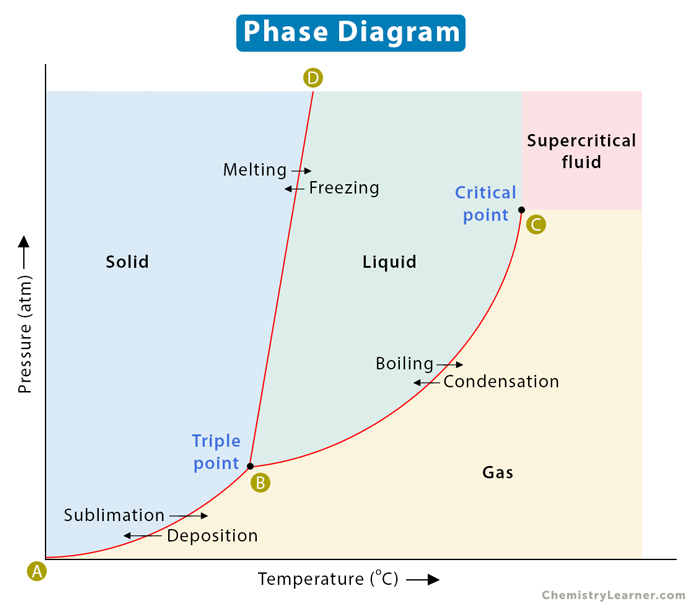
\includegraphics[width=1\columnwidth]{pd.jpg}
	\end{minipage}
\end{center}
		L'equazione di stato di van der Waals permette di descrivere proprio quello che succede attorno a questi punti critici; in realt\`a, permette di individuare proprio quel valore di temperatura, la temperatura critica, per cui, in un diagramma $(\rho ,T)$ si distinguono regioni in cui il sistema \`e gassoso (tipicamente a densit\`a basse), liquido (tipicamente a densit\`a alte) e in cui i due stati coesistono.

		In prossimit\`a dei punti critici, si vedr\`a che sar\`a possibile individuare la divergenza di alcune quantit\`a. 
		Per esempio, nelle vicinanze di punti critici, si possono osservare degli andamenti divergenti di alcune quantit\`a, come
		\[
		\begin{split}
			&k_T \sim \lvert T-T_C \rvert ^{-\gamma} \\
			& C_V \sim \lvert T-T_C \rvert ^{-\alpha }
		\end{split}
		\] 
	con $\gamma$ e $\alpha $ noti come \textit{esponenti critici}.
\subsection{Teoria di Lee-Yang}
Permette di individuare le transizioni di fase come singolarit\`a nella funzione di partizione.
Si parte dalla funzione di gran partizione, in quanto si intende studiare il sistema tramite il formalismo gran canonico; si ha 
\[
\mathcal{Z} (z,T,V) = \sum_{N=0}^{M} z^N Z(N,T,V)
\] 
con $z$ fugacit\`a, $Z$ la funzione di partizione canonica, e si deve avere $M<+\infty$ qualora il sistema sia finito, ossia nel caso in cui $V$ sia limitato\footnote{Questo perch\'e le particelle non possono sovrapporsi, quindi in un volume finito, se ne possono avere un numero finito.}.

Nel caso in cui la somma sia finita, non ci si aspettano comportamenti strani:
\[
\mathcal{Z} = 1+zZ(1,T,V) + z^2 Z(2,T,V) + \ldots + z^M Z(M,T,V) > 1
\] 
dove il $>1$ \`e dato dal fatto che $z=e^{\beta \mu }$ e le funzioni di partizione canoniche sono sempre positive.
Ne segue che $\mathcal{Z} $ \`e un polinomio di grado $M$ in $z$, per cui ammette esattamente $M$ radici nel campo complesso.
Indicando con $\xi _1,\ldots,\xi _M$ le sue radici, assumendo che siano tutte distinte, si pu\`o scrivere 
\[
\mathcal{Z} (z) = \prod_{N=1} ^M \left(1-\frac{z}{\xi _N}\right) 
\] 
Visto che $\mathcal{Z} (0) = 1$ e le $Z$ sono tutte positive, con $z>1$, si vede che le $\xi _k$ non possono appartenere alla retta reale positiva.
In realt\`a, quello che si pu\`o far vedere \`e che le radici sono a coppie di complessi coniugati, cio\`e se $\xi _j$ \`e radice, allora $\xi _j^*$ anche lo \`e.
Questo \`e dato dal fatto che la funzione di gran partizione deve essere una funzione reale, ossia invariante sotto coniugio complesso. 
Per il formalismo gran canonico, si ha
\[
\begin{cases}
	\displaystyle \frac{p}{\kappa _B T} = \frac{1}{V}\log\mathcal{Z} (z,T,V)\\
	\\
	\displaystyle \frac{1}{v}= \frac{\langle N \rangle}{V}=\frac{1}{V}z\frac{\partial }{\partial z} \log\mathcal{Z} (z,T,V)
\end{cases}
\] 
Ora, se $V$ \`e finito, quindi $N<+\infty$, non ci si aspettano singolarit\`a; anzi, il sistema \`e stabile: si ha $p>0$ e, essendo
\[
v = \frac{V}{z \partial _z \log\mathcal{Z} } \implies \Eval{\frac{\partial v}{\partial z} }{T}{} = -V \frac{\partial _z \log\mathcal{Z} + z \partial _z^2 \log\mathcal{Z} }{(z\partial _z\log\mathcal{Z} )^2}\\
\] 
vale
\[
	\begin{split}
		\Eval{\frac{\partial p}{\partial v} }{T}{} &=  \Eval{\frac{\partial p}{\partial z} \frac{\partial z}{\partial v} }{T}{} = \left(\frac{\kappa _B T}{V}\frac{\partial }{\partial z} \log\mathcal{Z} \right) \frac{1}{\Eval{\frac{\partial v}{\partial z} }{T}{}}\\
							   &= -\frac{\kappa _B T}{V^2}\frac{z^2 \left(\partial _z\log\mathcal{Z} \right) ^3}{\partial _Z \log\mathcal{Z} +z \partial _z^2 \log\mathcal{Z} } < 0
	\end{split}
\] 
Quest'ultima entra nella compresibilit\`a isoterma $k_T ^{-1} = - v \Eval{\frac{\partial p}{\partial v} }{T}{}$, che risulta, quindi, positiva, senza risultare in instabilit\`a.

Se, al contrario, nel limite termodinamico, le equazioni riportate sopra diventano:
\[
\begin{cases}
	\displaystyle \frac{p}{\kappa _B T }= \lim_{V \to +\infty} \frac{1}{V}\log\mathcal{Z} \\
	\\
	\displaystyle \frac{1}{v}=\lim_{V \to +\infty} \frac{1}{V} z \frac{\partial }{\partial z} \log\mathcal{Z} 
\end{cases}
\] 
In questo caso, il limite pu\`o causare problemi, anche perch\'e non \`e chiaro in principio se si possa scambiare con la derivata parziale, visto che la $\mathcal{Z} $, essendo ora una somma infinita di termini, pu\`o presentare punti di non analiticit\`a. 
La teoria di Lee-Yang prevede i seguenti teoremi, che permettono di capire quando nascono singolarit\`a.

\begin{teorema}
Il limite 
\[
\mathcal{F} (z) = \lim_{V \to +\infty} \frac{1}{V}\log\mathcal{Z} 
\] 
esiste per ogni valore di $z>0$. 
Inoltre, il risultato di tale limite \`e una funzione continua e non decrescente in $z$.
In generale, poi, $\mathcal{F} (z)$ non dipende da $V$, a patto che la sua superficie non aumenti pi\`u velocemente di $V^{2 / 3}$ (a meno di frattali, quindi).
\end{teorema}
\begin{teorema}
Se $R$ \`e una regione del piano complesso in cui non sono presenti zeri di $\mathcal{Z} $, allora $\mathcal{F} _V(z)$ converge uniformemente sui compatti di $R$, per $V\to +\infty$.
\end{teorema}
Come conseguenza di questo secondo teorema, la teoria matematica afferma che \`e possibile scambiare il limite con la derivata e questo corrisponde ai casi in cui non si verificano singolarit\`a.
Ne segue che, nella regione $R$, il sistema \`e termodinamicamente stabile, con 
\[
\frac{p}{\kappa _B T } = \mathcal{F}(z) \hspace{1cm} v^{-1}(z) = z \frac{\partial }{\partial z} \mathcal{F} (z)
\] 
e si pu\`o dimostrare che $p>0$ e $\frac{\partial p}{\partial v}  < 0$.

Per evidenziare la stabilit\`a termodinamica in $R$, si nota che, il primo teorema assicura $\frac{\partial p}{\partial z} \ge  0$, cio\`e $p(z)$ \`e una funzione crescente; inoltre, si pu\`o vedere che $v^{-1}$ non decresce in funzione di $z$ perch\'e
\[
z \frac{\partial }{\partial z} \frac{1}{v}= z \frac{\partial }{\partial z} \left(z \frac{\partial }{\partial z} \frac{1}{V}\log\mathcal{Z} \right) \propto \operatorname{Var} N
\] 
per quanto visto nella trattazione del formalismo gran canonico. Visto che le fluttuazioni di $N$ devono essere positive, allora $v^{-1}$ deve essere crescente in $z$ (cio\`e $\partial _z v^{-1}\ge 0$).
Combinando questi due risultati, eliminando la fugacit\`a, si ottiene $\frac{\partial p}{\partial v} \le 0$, cio\`e la pressione decresce con l'aumentare del volume, il che individua una regione di stabilit\`a termodinamica per il sistema.

Quello che la teoria di Lee-Yang permette di comprendere \`e che, se $V<+\infty$, la funzione di gran partizione \`e analitica in $z$, quindi neanche $p$ e $v$.
Nel caso in cui $V\to +\infty$, invece, gli zeri di $\mathcal{Z} (z)$ possono accumularsi e tendere arbitrariamente vicino all'asse reale; questo significa che esister\`a un punto di tale asse reale attorno al quale non si riesce a trovare una regione libera da zeri.
Questo punto reale \`e proprio il punto critico ed \`e dove si verificano le transizioni di fase.
\begin{teorema}
	[Teorema del cerchio]
	Per un sistema con particelle disposte a reticolo (cio\`e senza sovrapporsi) e soggette a potenziale della forma 
	\[
	v_{ij} = \begin{cases}
		+\infty &,\ i=j\\
		<0 &,\ i\neq j
	\end{cases}
	\] 
	allora $\mathcal{Z} (z,T,V) = 0 \iff \lvert z \rvert =1$.
\end{teorema}
\begin{osservazione}
Questo teorema permette di concludere che un'eventuale transizione di fase, per un sistema del tipo previsto dal teorema, pu\`o verificarsi esclusivamente per $z=1$, visto che gli zeri di $\mathcal{Z} (z)$ sono sulla circonferenza unitaria in $\mathbb{C}$.
\end{osservazione}
\noindent Se $\theta _k$ sono le fasi delle radici di $\mathcal{Z} $, allora, nel caso del potenziale considerato sopra, si pu\`o scrivere, imponendo anche $\mathcal{Z} (0) = 1$, che
\[
\mathcal{Z}  = \prod_k \frac{z-e^{i\theta _k}}{- e ^{-i\theta _k}}
\] 
Essendo interessati al limite termodinamico, per\`o, la produttoria non va pi\`u bene perch\'e \`e su indice discreto.
L'idea \`e di definire una funzione di distribuzione $g(\theta )$, con $\theta \in [0,2\pi)$, che indica come sono distribuiti gli zeri nel limite termodinamico.
Inoltre, essendo le radici di $\mathcal{Z} (z)$ coppie di complessi coniugati, deve valere anche
\[
g(\theta ) = g(-\theta )
\] 
In questo modo, nel limite termodinamico, si ha:
\[
\log\mathcal{Z} =\sum_{k}^{} \log \left(\frac{z-e^{-i\theta _k}}{-e ^{-i\theta _k}}\right) \longrightarrow V \int_{0} ^{2\pi} d\theta  \ g(\theta ) \log\left(\frac{z- e^{-i\theta }}{-e^{-i\theta }}\right) 
\] 
Visto che $g(\theta )=g(-\theta )$, l'integrale tra $0$ e $\pi$ sar\`a uguale a quello tra $\pi$ e $2\pi$.
Ne segue che
\[
	\begin{split}
		\log \mathcal{Z}  &= V \int_{0} ^{\pi} d\theta \ g(\theta ) \log \left(\frac{z-e^{-i\theta }}{-e^{-i\theta }}\right) + V \int_{\pi}^{2\pi} d\theta \ g(\theta ) \log \left(\frac{z-e^{-i\theta}}{-e^{-i\theta }}\right)  \\
				  &= V \int_{0} ^{\pi} d\theta \ g(\theta ) \log \left(\frac{z-e^{-i\theta }}{-e^{-i\theta }}\right) + V \int_{0}^{\pi} d\theta \ g(-\theta ) \log \left(\frac{z-e^{i\theta}}{-e^{i\theta }}\right) \\
				  &=V \int_{0} ^\pi d\theta \ g(\theta ) \log \left[ \frac{z-e^{-i\theta }}{-e^{-i\theta }} \frac{z- e^{i\theta }}{- e^{i\theta }} \right] \\
				  &= V \int_{0} ^\pi d\theta  \ g(\theta ) \log\left(z^2 + 1 - 2z \cos \theta \right) 
	\end{split}
\] 
In questo modo, si ottiene che
\[
\begin{cases}
	\displaystyle \frac{p}{\kappa _B T} = \int_{0} ^\pi d\theta \ g(\theta ) \log\left(z^2 + 1 - 2z \cos \theta \right) \\
	\\
	\displaystyle \frac{1}{v} = \frac{1}{V}z\frac{\partial }{\partial z} \log\mathcal{Z}  = 2z \int_{0} ^\pi d\theta \ g(\theta ) \frac{z-\cos \theta }{z_2 + 1 - 2z \cos \theta }
\end{cases}
\] 
Da queste formule, si deduce che la singolarit\`a pu\`o avvenire solamente nel punto $(\theta ,z) = (0,1)$, quando $g(\theta =0) \neq 0 $.
Inoltre, tutte le informazioni sul sistema si ottengono a partire dalla conoscenza di $g(\theta )$.
\subsection{Esponenti critici in van der Waals}
Si considera il caso di van der Waals con tutte le assunzioni del caso. 
In prossimit\`a del punto critico, vale la legge degli stati corrispondenti:
\[
\left(\overline{P}+\frac{3}{\overline{V}^2}\right) \left(\overline{V}-\frac{1}{3}\right) = \frac{8}{3}\overline{T}
\] 
con $\overline{P}= P / P_c$, $\overline{V}= V / V_c$ e $\overline{T} = T / T_c$.
Si definiscono le variabili ridotte
\[
 p = \frac{P-P_c}{P_c}\hspace{1cm}v = \frac{V-V_c}{V_c} \hspace{1cm} t = \frac{T-T_c}{T_c}
\] 
e si assume di essere arbitrariamente vicini al punto critico $(T_c,V_c,P_c)$.
In fisica, sono attualmente noti 6 \textit{esponenti critici}; nella seguente trattazione, se ne evidenzieranno 4 che caratterizzano la classe delle transizioni di fase di cui fa parte van der Waals (cio\`e che \`e descritto da van der Waals).
\begin{enumerate}[(1).]
	\item Se $t=0$, allora
		\[
		\frac{\partial P}{\partial V} = \frac{\partial ^2P}{\partial V^2} = 0
		\] 
		perch\'e, nel punto critico, si ha un punto di flesso nel diagramma $(V,P)$ a $T=T_C$ (cio\`e $t=0$).
		Ne segue che 
		\[
		p \sim v^\delta 
		\] 
		con $\delta = 3$. 
		Per verificarlo, basta imporre $T=T_c$ nella legge degli stati corrispondenti e studiare l'andamento di $p(v)$.
		Infatti, essendo $T=T_c$, vale $\overline{T}=1$ e 
		\[
		\overline{P} = \frac{8}{2\overline{V}-1}- \frac{3}{\overline{V}^2}
		\] 
		Visto che $\overline{V}= 1+v$, si ha $3 \overline{V}-1 = 2 + 3v$, per cui
		\[
		\frac{8}{3\overline{V}-1}= 4 \left(1 + \frac{3}{2}v\right) ^{-1}\hspace{1cm} \frac{3}{\overline{V}^2} = 3 ( 1+ v)^{-2}
		\] 
	Essendo arbitrariamente vicini al punto critico, si usano gli sviluppi $(1+x)^{-1} = 1- x + x^2 -x^3 +\ldots$ e $(1+x)^{-2} = 1 - 2x + 3x^2 - 4x^3 +\ldots$:
\[
\frac{8}{3\overline{V}-1} \simeq 4 - 6v + 9 v^2 - \frac{27}{2}v^3 \hspace{1cm} \frac{3}{\overline{V}^2}\simeq 3 - 6 v + 9 v^2 - 12 v^3
\] 
Allora
\[
\overline{P}\simeq \left(4 - 6v + 9 v^2 - \frac{27}{2}v^3\right) -\left(3 - 6 v + 9 v^2 - 12 v^3\right) = 1 - \frac{3}{2}v^3
\] 
Visto che $p = \overline{P}-1$, si ha $p \simeq -\frac{3}{2}v^3$, per cui $p \sim v^3$\footnote{Tecnicamente sarebbe $\lvert p \rvert \sim\lvert v \rvert ^{\delta }$, con $\delta = 3$, ma il modulo \`e implicito in $p\sim v^3$.}.
	\item Si ricorda che
		\[
			C_V = T \Eval{\frac{\partial S}{\partial T} }{V}{} = \Eval{\frac{\partial U}{\partial T} }{V}{}
		\] 
		Nel caso di van der Waals, si ricorda che l'energia interna \`e pari a 
		\[
		U = \frac{3}{2}N \kappa _B T - \frac{\partial }{\partial \beta } \log Z_N = \frac{3}{2}N \kappa _B T + \frac{\partial }{\partial \beta } \left(\frac{N^2}{2}\frac{a}{V}\right) 
		\] 
		con 
		\[
		a = 4\pi \int dr \ r^2 \left(1- e ^{-\beta  v(r)}\right) \simeq 4\pi \beta  \int dr \ r^2 v(r)
		\] 
		visto che la teoria \`e in regime di $\lvert \kappa _B T \rvert \gg \lvert v(r) \rvert $.
		Quindi 
		\[
		U \simeq \frac{3}{2} N \kappa _B T + \frac{N^2}{V} 2\pi \int dr \ r^2 v(r)
		\] 
		e, allora
		\[
		C_V = \frac{3}{2}N \kappa _B \implies C_V \sim t ^{-\alpha }
		\] 
		con $\alpha  = 0$ in questo caso perch\'e risulta costante.
	\item La compressibilit\`a isoterma \`e pari a
		\[
			k_T = - \frac{1}{V \Eval{\frac{\partial p}{\partial V} }{T}{}}
		\] 
		con 
		\[
			\Eval{\frac{\partial p}{\partial V} }{T}{} = - \frac{N\kappa _B T}{(V-b)^2}+ \frac{2a}{V^3}=\frac{N\kappa _B}{4b^2}(T_c-T)
		\] 
		utilizzando il valore $T_c = \frac{8}{27}\frac{a}{b}\frac{1}{N\kappa _B}$ e il fatto che $V = V_c = 3b$, essendo interessati al comportamento di $k_T$ nei pressi del punto critico.
		Questo implica che 
		\[
		k_T \sim \lvert t \rvert ^{-\gamma}
		\] 
		con $\gamma=1$.
		Questo significa che $k_T$ diverge in prossimit\`a del punto critico, comportando forti fluttuazioni nel numero di particelle e invalidando, allora, l'equivalenza del gran canonico con gli altri ensemble.
	\item Si va a studiare il caso in cui gas e liquido coesistono secondo il diagramma $(\rho ,T)$. 
		\begin{center}
			\begin{minipage}
				{.45\columnwidth}
				Si \`e interessati a capire qual \`e l'andamento della densit\`a del liquido $\rho _\text{liq}$ e del gas $\rho _\text{gas}$ nel tendere al punto critico, percorrendo la cupola della parabola.
				In particolare, si stimer\`a la differenza $\rho _\text{liq}- \rho _\text{gas}$ in funzione della temperatura.
				Per farlo, si considera $T<T_c$, visto che, sopra questo valore, il sistema \`e nello stato gassoso e, quindi, non c'\`e coesistenza.
			\end{minipage}
			\hfill
			\begin{minipage}
				{.45\columnwidth}
				\centering
		\begin{tikzpicture}[>=Stealth, line cap=round, line join=round, scale=.8]

    % Assi
    \draw[->, thick] (0,0) -- (0,5) node[above] {$T$};
    \draw[->, thick] (0,0) -- (7,0) node[right] {$\rho$};

    % Linea critica Tc
    \draw[dashed, thick] (0,3.55) -- (6.7,3.55);
    \node[left] at (0,3.55) {$T_c$};

    % Curva a cupola (coexistence dome)
    \draw[thick]
        (1.0,1.1)
        .. controls (1.7,2.7) and (2.6,3.4) .. (3.5,3.55)
        .. controls (4.4,3.4) and (5.2,2.7) .. (6.0,1.1);

    % Punto critico
    \fill[red] (3.5,3.55) circle (2.2pt);

    % Etichette
    \node at (0.55,1.75) {\footnotesize gas};
    \node at (6.75,1.75) {\footnotesize liquido};
    \node at (3.5,1.75) {\footnotesize coesistenza};
    \node at (3.45,4) {\footnotesize gas};

\end{tikzpicture}
			\end{minipage}
		\end{center}
Invertendo la legge degli stati corrispondenti, si vede che
\[
\frac{P}{P_c}=\frac{8 T / T_c}{3 \overline{V}-1}- \frac{3}{\overline{V}^2}
\] 
Da van der Waals e a seguito della costruzione di Maxwell, si sa che ci sono una serie di volumi che corrispondono tutti alla stessa pressione, i cui estremi corrispondono ad uno stato gassoso (a sinistra) e uno stato liquido (a destra).
Per questa ragione, tale equazione sar\`a soddisfatta da entrambi questi volumi, ottenendo che
\[
	\begin{split}
		&\frac{P}{P_c} = \frac{8 T / T_c}{3 \overline{V}_\text{liq}-1} - \frac{3}{\overline{V}_\text{liq}^2}= \frac{8 T / T_c}{3 \overline{V}_\text{gas}-1} - \frac{3}{\overline{V}_\text{gas}^2}\\
		&\Rightarrow \frac{T}{T_c} = \frac{\left(3\overline{V}_\text{liq}-1\right) \left(3\overline{V}_\text{gas}-1\right) \left(\overline{V}_\text{liq}+\overline{V}_\text{gas}\right) }{8 \overline{V}^2_\text{gas} \overline{V}^2_\text{liq}}
	\end{split}
\] 
		\begin{center}
			\begin{minipage}
				{.45\columnwidth}
Si suppone, ora, che $\overline{V}_\text{gas} = \frac{V_c+\varepsilon }{V_c}$ e $\overline{V}_\text{liq}=\frac{V_c-\varepsilon }{V_c}$, ossia che questi due valori si discostino di un arbitrario $\varepsilon >0$ rimanendo sulla parabola, cio\`e lungo la retta per cui restituiscono uguale pressione in regime di coesistenza.
In questo caso, si pu\`o approssimare 
\[
\frac{T}{T_c} = 1- \frac{\varepsilon ^2}{4V_c^2}+ \operatorname{O} (\varepsilon ^4)
\] 
			\end{minipage}
			\hfill
			\begin{minipage}
				{.45\columnwidth}
				\centering
\begin{tikzpicture}[>=Stealth, line cap=round, line join=round, scale=.8]

% Assi
\draw[->, thick] (0,0) -- (0,5) node[above] {$T$};
\draw[->, thick] (0,0) -- (7,0) node[right] {$V$};

% Cupola (coexistence dome)
\draw[thick]
    (1.2,1.0)
    .. controls (2.0,2.8) and (3.0,3.6) .. (3.8,3.7)
    .. controls (4.6,3.6) and (5.5,2.8) .. (6.2,1.0);

% Punto critico (rosso)
\fill[red] (3.8,3.7) circle (2.2pt);

% Punto sulla curva (nero)
\fill (5.1,2.9) circle (2pt);
\fill (2.5,2.9) circle (2pt);

% Linea orizzontale tratteggiata dal punto nero
\draw[dashed] (0,2.9) -- (5.1,2.9);

% Linea verticale tratteggiata (azzurra)
\draw[dashed, blue] (5.1,0) -- (5.1,2.9);
\draw[dashed, blue] (2.5,0) -- (2.5,2.9);

% Linea verticale da punto critico a asse x
\draw[dashed] (3.8,3.7) -- (3.8,0);

% Etichette
\node at (1.3,3.1) {\footnotesize liq.};
\node at (6.5,3.0) {\footnotesize gas};
\node at (3.25,1.9) {\footnotesize coes.};

% Etichetta Vc
\node[below] at (3.8,0) {$V_c$};

% Frecce epsilon (a sinistra e destra di Vc)
\draw[<->, blue] (2.5,-1) -- (3.8,-1);
\draw[<->, blue] (3.8,-1) -- (5.1,-1);

\node[blue] at (3.15,-1.3) {$\varepsilon$};
\node[blue] at (4.45,-1.3) {$\varepsilon$};

\end{tikzpicture}
			\end{minipage}
		\end{center}
Da questa, si ricava che 
\[
\varepsilon \sim -t ^{\beta }
\] 
con $\beta  = 1 / 2$. 
Questa, in particolare, \`e valida per $t<0$, ossia per valori $T<T_c$; si vede che, per $t>0$, si ha $\varepsilon = 0$.
\end{enumerate}
Si far\`a vedere, nel seguito, un altro sistema i cui esponenti $\alpha ,\beta ,\gamma, \delta $ sono gli stessi di questo, anche se il sistema in questione si studia sotto tutt'altro punto di vista, ossia transizioni di fase che riguardano le sue propriet\`a magnetiche.
Questo \`e dovuto al fatto che i due sistemi fanno parte della stessa \textit{classe di universalit\`a}, il che ha a che fare con le assunzioni sul sistema, pi\`u che l'aspetto che se ne intende studiare.
Di fatto, si riutilizzeranno le assunzioni di gas rarefatto, approssimato al primo ordine dell'espansione in clusters, eccetera.
\subsection{Modello di Ising in campo medio}
Per schematizzare in modo elementare un sistema magnetico in meccanica statistica classica, si introducono delle variabili $S_i$ che possono assumere valori esclusivamente pari a $\pm 1$.
L'idea \`e di assegnare queste variabili ad ogni particella all'interno di un reticolo e determiner\`a il comportamento della particella ad allinearsi con il campo magnetico esterno.
Il modello di Ising \`e caratterizzato da un hamiltoniana 
\[
H = - J \sum_{\langle i,j \rangle}^{} S_iS_j - h \sum_{i}^{} S_i
\] 
dove $J$ \`e la costante di accoppiamento, $\langle i,j \rangle$ somma, dato $i$, sui prossimi vicini alla particella $i$-esima nel reticolo (cio\`e sulle particelle \textit{connesse} alla $i$-esima direttamente), e $h$ \`e il campo magnetico.
Se $J>0$, il sistema sar\`a ferromagnetico perch\'e $H$ assume valore minimo quando la particella $i$-esima \`e allineata con i suoi vicini, altrimenti, per $J<0$, si ha un comportamento anti-ferromagnetico. 


		\begin{center}
			\begin{minipage}
				{.45\columnwidth}
Prendendo $h=0$ e $J>0$, si pu\`o osservare una transizione da paramagnete (ordinamento casuale degli $S_i$) a ferromagnete passando da alte temperature ($\beta \sim 0$) a basse temperature ($\beta \to  +\infty$).
Questo individua una transizione di fase per cui la magnetizzazione $m$, che si trover\`a essere $\langle S_i \rangle$ (valor medio), ha un punto di discontinuit\`a ad una certa $T_c$, sopra cui \`e costante e pari a zero.
			\end{minipage}
			\hfill
			\begin{minipage}
				{.45\columnwidth}
				\centering
				\begin{tikzpicture}[>=Stealth, line cap=round, line join=round, scale=.8]

% Assi
\draw[->, thick] (0,0) -- (7,0) node[right] {$T$};
\draw[->, thick] (0,0) -- (0,5) node[above] {$\langle S_i \rangle$};

% Punto critico
\coordinate (Tc) at (3.2,0);
\fill (Tc) circle (2pt);

% Etichetta Tc
\node[below] at (Tc) {$T_c$};

% Curva (fase ordinata) - rossa
\draw[thick, red]
    (0,3.6)
    .. controls (1.5,3.4) and (2.5,2.2) .. (3.2,0);

% Linea per T > Tc (fase disordinata) - blu
\draw[thick, blue] (3.2,0) -- (6.5,0);

% Etichetta punto critico con freccia
\draw[->] (4.8,2.5) -- (3.25,0.1);
\node at (5.2,2.7) {\footnotesize punto critico};

\end{tikzpicture}
\captionof{figure}{Magnetizzazione in funzione della temperatura.}
\label{m-T}
			\end{minipage}
		\end{center}
		In realt\`a, non \`e sistematico che si verifichi questo andamento, ma dipende dal tipo di reticolo considerato.
\subsubsection{Soluzione del modello di Ising}
Per risolvere il modello di Ising, ossia calcolare tutte le quantit\`a termodinamiche necessarie, \`e necessario determinare 
\[
Z = \sum_{\left\{ S_i \right\} }^{} e^{-\beta H\left(\left\{ S_i \right\} \right) }
\] 
\begin{osservazione}
Si usa il formalismo canonico perch\'e il numero di particelle \`e fissato dal numero di reticoli del sistema.
\end{osservazione}
\noindent Si definisce la magnetizzazione del sito $i$-esimo come $m_i = \langle S_i \rangle$; in questo modo, si pu\`o esprimere ogni variabile $S_i$ in termini del suo valor medio e delle sue fluttuazioni come 
\[
S_i = m_i + \delta S_i
\] 
Calcolare la somma per ottenere $Z$ \`e molto difficile, per cui si fa uso dell'approssimazione di Weiss (o di campo medio), per cui si assume che le $\delta S_i$ siano molto piccole.
Si ha
\[
H = - J  \sum_{\langle i,j \rangle}^{} S_iS_j - h \sum_{i=1}^{N} S_i = - J \sum_{\langle i,j \rangle}^{} (m_i + \delta S_i) (m_j + \delta S_j) - h \sum_{i=1}^{N} (m_i+ \delta S_i)
\] 
Assumendo anche invarianza per traslazioni, si pu\`o scrivere che $m_i = m, \ \forall i$.
Sviluppando il prodotto e semplificando il secondo ordine delle fluttuazioni per l'approssimazione di campo medio, si trova:
\[
	\begin{split}
		m_i m_j + m_i \delta S_j + m_j \delta S_i + \cancel{\delta S_i \delta S_j}&=m^2 + m(\delta S_i + \delta S_j)\\
											  &=m^2 + m \big[ (S_i - m) + (S_j - m) \big] \\
											  &= -m^2 + m(S_i + S_j)
	\end{split}
\] 
In questo modo, si ha
\[
	\begin{split}
		H &\simeq - J \sum_{i=1}^{N} \sum_{j_\text{p.v.}}^{} (-m^2+2mS_i) - h \sum_{i=1}^{N} S_i\\
		  &= - J y \frac{1}{2} \sum_{i=1}^{N} (-m^2+2mS_i) - h \sum_{i=1}^{N} S_i\\
		  &= \frac{1}{2}Jy m^2 N - (h + mJy) \sum_{i=1}^{N} S_i
	\end{split}
\] 
dove $j_\text{p.v.}$ indica le particelle $j$-esime prime vicine con la $i$-esima e $y$ \`e il numero di primi vicini di un sito nel reticolo.
Il fattore $\frac{1}{2}$ serve per evitare di contare due volte le stesse coppie di particelle.
Il fattore $h+mJy$ si dice \textit{campo magnetico efficace} ed \`e importante notare che dipende dalla magnetizzazione $m$ del sistema.
Allora 
\begin{equation}\label{cic}
	\begin{split}
		Z &= C \sum_{\left\{ S_i \right\} }^{} e^{\beta (h + mJy) \sum_{i}^{} S_i} = C \prod_i \sum_{S_i = \pm 1}^{} e^{\beta (h+mJy)S_i}\\
		  &=C \prod_i \left[ e^{\beta (h+mJy)}+ e ^{-\beta (h+mJy)} \right] = 2^N C \cosh\left(\beta h + \beta mJy\right) ^N
	\end{split}
\end{equation}
dove $C$ \`e una costante moltiplicativa legata alla presenza del termine costante (rispetto alle quantit\`a termodinamiche di interesse) $\frac{1}{2}Jy m^2 N$ nell'hamiltoniana.
Dalla termodinamica, la magnetizzazione del sistema \`e pari a 
\begin{equation}\label{mising}
m = \frac{1}{N} \left(\frac{1}{\beta }\frac{\partial }{\partial h} \log Z\right) _{h=0}  = \tanh \left(\beta h + \beta m Jy\right)_{h=0} =\tanh \left(\beta mJy\right) 
\end{equation}
e si vede che la magnetizzazione compare sia a destra che a sinistra.
\begin{center}
	\begin{minipage}
		{.45\columnwidth}
		\centering
\begin{tikzpicture}[scale=1]
    % Assi coordinati
    \draw[->, thick] (-3,0) -- (3,0) node[right] {$m$};
    \draw[->, thick] (0,-1.5) -- (0,1.5) node[left] {$f(m)$};

    % Retta y=m
    \draw[thick] (-1.2,-1.2) -- (1.2,1.2) node[above right] {\footnotesize$f(m)=m$};
    \draw[dashed] (-1.5,-1.5) -- (-1.2,-1.2);
    \draw[dashed] (1.2,1.2) -- (1.5,1.5);

    % Curva y=tanh(...) con pendenza < 1
    \draw[domain=-2:2, samples=100, thick, cyan!80!blue] plot (\x, {1.5*tanh(0.4*\x)});
    \draw[dashed, cyan!80!blue] (2, {1.5*tanh(0.4*2)}) -- (2.5, {1.5*tanh(0.4*2.5)});
    \draw[dashed, cyan!80!blue] (-2, {1.5*tanh(0.4*-2)}) -- (-2.5, {1.5*tanh(0.4*-2.5)});
    
    % Etichetta curva
    \node[cyan!80!blue, right] at (0.8, 0.4) {\footnotesize$f(m)=\tanh(\beta m J y)$};

    % Origine e radice banale
    \fill[red] (0,0) circle (1.5pt) node[below right] {\footnotesize$m=0$};
\end{tikzpicture}
	\end{minipage}
	\hfill
	\begin{minipage}
		{.45\columnwidth}
		\centering
		\begin{tikzpicture}[scale=1]
    % Assi coordinati
    \draw[->, thick] (-3,0) -- (3,0) node[right] {$m$};
    \draw[->, thick] (0,-1.5) -- (0,1.5) node[left] {$f(m)$};

    % Retta y=m
    \draw[thick] (-1.2,-1.2) -- (1.2,1.2);
    \draw[dashed] (-1.5,-1.5) -- (-1.2,-1.2);
    \draw[dashed] (1.2,1.2) -- (1.5,1.5);

    % Curva y=tanh(...) con pendenza > 1
    \draw[domain=-2:2, samples=100, thick, cyan!80!blue] plot (\x, {1.5*tanh(\x)});
    \draw[dashed, cyan!80!blue] (2, {1.5*tanh(2)}) -- (2.5, {1.5*tanh(2.5)});
    \draw[dashed, cyan!80!blue] (-2, {1.5*tanh(-2)}) -- (-2.5, {1.5*tanh(-2.5)});

    % Punti di intersezione
    \fill[red] (0,0) circle (1.5pt) node[below right] {\footnotesize$m=0$};
    \fill[red] (1.293,1.293) circle (1.5pt);
    \fill[red] (-1.293,-1.293) circle (1.5pt);

    % Linee di proiezione sulle ascisse
    \draw[dashed, red] (1.293,1.293) -- (1.293,0) node[below right] {\footnotesize$+m^*$};
    \draw[dashed, red] (-1.293,-1.293) -- (-1.293,0) node[above left] {\footnotesize$-m^*$};
\end{tikzpicture}
\end{minipage}
\end{center}
Questi due grafici individuano i due casi possibili, a seconda del coefficiente angolare della retta $f(m) = m$.
Il caso a sinistra \`e associato a 
\[
	\Eval{\frac{\partial \tanh(\beta mJy)}{\partial m} }{m=0}{} <1 \iff \beta J y <1
\] 
mentre il secondo caso \`e individuato dalla condizione 
\[
	\Eval{\frac{\partial \tanh(\beta mJy)}{\partial m} }{m=0}{} >1 \iff \beta J y >1
\] 
Questa differenza tra i valori possibili della magnetizzazione permette di individuare una temperatura critica:
\[
\beta _c Jy = 1 \iff \frac{1}{\kappa _B T_c}Jy = 1 \iff T_c  = \frac{Jy}{\kappa _B}
\] 
che coincide proprio con la temperatura critica a cui avviene la transizione di fase introdotta alla fine della scorsa sezione.
\begin{osservazione}
	I valori $m^*$ e $-m^*$ sono simmetrici e sono legati al fatto che il grafico di $m(T)$ a fine della scorsa lezione pu\`o avere un ramo rosso nella parte superiore del piano, o uno perfettamente specchiato nella parte inferiore.
\end{osservazione}
\noindent In particolare, il caso $T>T_c \Rightarrow m=0$ corrisponde al caso paramagnetico, mentre il caso $T<T_c$, che permette $m=0, +m^*, - m^*$, corrisponde al caso ferromagnetico.
Per capire quali di queste soluzioni sono fisicamente ammissibili (nel caso $T<T_c$), si studia l'energia libera e si vede a quali di queste corrisponde un suo minimo.
L'energia libera \`e data da
\[
	\begin{split}
		F &= -\kappa _B T \log Z = \frac{1}{2} Jy N m^2 - \kappa _B T N \log \Big[2\cosh\big(\beta h+\beta mJy\big)\Big]\\
		  &= F_0 + \frac{a}{2}m^2 + \frac{b}{4!}m^4 - \lambda hm + \ldots
	\end{split}
\] 
dove si \`e usato lo sviluppo per $h,m \ll 1$ e che $\log(\cosh \epsilon ) = \frac{\epsilon ^2}{2}- \frac{\epsilon ^4}{12}+\ldots$ per $\epsilon \ll 1$.
In questa espressione, si ha
\[
F_0=-N\kappa _B T \log 2 \hspace{.5cm} a = N \frac{Jy}{\kappa _B T } \left(\kappa _B T - Jy\right)  \hspace{.5cm} b = 2N \kappa _B T \left(\frac{Jy}{\kappa _B T}\right) ^4 \hspace{.5cm}\lambda = 2N \frac{Jy}{\kappa _B T}
\] 
con $a \sim T-T_c$, visto che $T_c = Jy / \kappa _B$.
Si nota che l'equazione $m=\tanh(\beta mJy)$ equivale alla condizione 
\[
	\Eval{\frac{\partial F}{\partial m} }{h=0}{} = 0 \iff \cancel{JyN}m - \kappa _B T \cancel{N} \frac{\big[ \sinh(\beta mJy) \big] \beta \cancel{Jy}}{\cosh(\beta mJy)}=0 \iff m - \tanh(\beta mJy) = 0
\] 
quindi i valori $m=0,m^*,-m^*$ sono gi\`a punti stazionari.
Dallo sviluppo di $F$, si vede che, essendo $b,\lambda >0$ e $F_0 < 0$, si possono avere due casi distinti:
\begin{itemize}
	\item se $T>T_c$, ossia $a>0$, $F$ \`e una quartica con concavit\`a verso l'alto e un unico minimo:
\begin{center}
			\begin{minipage}
				{.45\columnwidth}
				\centering
				\begin{tikzpicture}[>=Stealth, line cap=round, line join=round, scale=.8]

% Assi
\draw[->, thick] (-3,0) -- (3,0) node[right] {\footnotesize$m$};
\draw[->, thick] (0,-3) -- (0,3) node[above] {\footnotesize$F$};

% Parabola principale
\draw[thick] plot[domain=-2:2, samples=100] (\x, {0.8*\x*\x - 2});

% Ramo tratteggiato (continuazione metastabile)
\draw[dashed] plot[domain=1.2:2.2, samples=50] (\x, {0.8*\x*\x - 2});
\draw[dashed] plot[domain=-2.2:-1.2, samples=50] (\x, {0.8*\x*\x - 2});

% Punto minimo
\fill[red] (0,-2) circle (2pt);

% Etichette
\node at (2.2,3) {\footnotesize$[h=0]$};
\node[below right] at (0,0) {\footnotesize$0$};
\node[below] at (.5,-2) {\footnotesize$F_0$};
\node[below] at (-0.7,-2) {\footnotesize$m=0$};

\end{tikzpicture}
			\end{minipage}
			\hfill
			\begin{minipage}
				{.45\columnwidth}
				\centering\begin{tikzpicture}[>=Stealth, line cap=round, line join=round, scale=.8]

% Assi
\draw[->, thick] (-3,0) -- (3,0) node[right] {\footnotesize$m$};
\draw[->, thick] (0,-3) -- (0,3) node[above] {\footnotesize$F$};

% Parabola inclinata (campo esterno)
\draw[thick] plot[domain=-2:2, samples=100] (\x, {0.8*\x*\x - 0.8*\x - 1.5});

% Rami tratteggiati (continuazioni)
\draw[dashed] plot[domain=1.2:2.2, samples=50] (\x, {0.8*\x*\x - 0.8*\x - 1.5});
\draw[dashed] plot[domain=-2.2:-1.2, samples=50] (\x, {0.8*\x*\x - 0.8*\x - 1.5});

% Etichetta
\node at (2.2,3) {\footnotesize$[h\neq 0]$};

\end{tikzpicture}
			\end{minipage}
\end{center}
	\item se $T<T_c$, ossia $a<0$, $F$ ha due punti di minimo, $\pm m^*$ e $m=0$ \`e un massimo locale, con la particolarit\`a che, quando $h\neq 0$, uno di questi due punti di minimo viene favorito dal sistema, a seconda della sua tendenza ad allinearsi o meno col campo magnetico esterno:
\begin{center}
			\begin{minipage}
				{.45\columnwidth}
				\centering
				\begin{tikzpicture}[>=Stealth, line cap=round, line join=round, scale=.9]

% Assi
\draw[->, thick] (-3,0) -- (3,0) node[right] {\footnotesize$m$};
\draw[->, thick] (0,-3) -- (0,3) node[above] {\footnotesize$F$};

% Potenziale a doppio minimo (quartico)
\draw[thick] plot[domain=-2.1:2.1, samples=200]
    (\x, {0.4*(\x*\x - 1.2)^2 - 1.8});

% Minimi
\fill[red] (-1.1,-1.8) circle (2pt);
\fill[red] (1.1,-1.8) circle (2pt);
\fill[red] (0,-1.225) circle (2pt);

% Linee verticali tratteggiate (m*)
\draw[dashed, red] (-1.1,0) -- (-1.1,-1.8);
\draw[dashed, red] (1.1,0) -- (1.1,-1.8);

% Etichette
\node at (2.2,2.8) {\footnotesize$[h=0]$};
\node at (-1.1,0.4) {\footnotesize$-m^*$};
\node at (1.1,0.4) {\footnotesize$+m^*$};
\node at (0.2,-1) {\footnotesize$F_0$};

\end{tikzpicture}
			\end{minipage}
			\hfill
			\begin{minipage}
				{.45\columnwidth}
				\centering
\begin{tikzpicture}[>=Stealth, line cap=round, line join=round, scale=.9]

% Assi
\draw[->, thick] (-3,0) -- (3,0) node[right] {$m$};
\draw[->, thick] (0,-3) -- (0,3) node[above] {$F$};

% Parametro (campo)
\def\h{0.6}

% Funzione
\draw[thick, domain=-1.6:1.8, samples=200]
    plot (\x, {(\x*\x -1)^2 - \h*\x -1.5});


% Minimi (posizionati manualmente ma coerenti)
\coordinate (minR) at (1.066, {((1.066*1.066-1)^2 - \h*1.066 -1.5)});
\coordinate (minL) at (-0.915, {((-0.915*-0.915-1)^2 - \h*(-0.915)-1.5)});

% Linee verticali tratteggiate (m*)
\draw[dashed, red] (-0.915,0) -- (-0.915,{((-0.915*-0.915-1)^2 - \h*(-0.915)-1.5)});
\draw[dashed, red] (1.066,0) -- (1.066,{((1.066*1.066-1)^2 - \h*1.066 -1.5)});


% Punto stabile (minimo globale)
\fill[red] (minR) circle (2.2pt);

% Punto metastabile (minimo locale)
\draw[red, thick] (minL) circle (2.2pt);

% Etichetta
\node at (2.2,3) {\footnotesize$[h\neq 0]$};

\end{tikzpicture}
			\end{minipage}
\end{center}
\end{itemize}
In assenza di campo magnetico, il valore $m^* \to 0$ con continuit\`a per $T\to T_c^-$ e si ottiene proprio un grafico simile a quello in figura \ref{m-T}.
In realt\`a, quando $h=0$, come gi\`a accennato, si potrebbe creare un andamento speculare (specchiato) per $m<0$, corrispondente all'andamento di $-m^*$, visto che l'energia libera \`e simmetrica per scambio di segno in $m$.
Quando si prende $h\neq 0$, per\`o, si ha una rottura della simmetria del sistema: la comparsa del termine lineare in $F$ evidenzia una preferenza per un valore di $m$, che sia positivo o negativo.
Questo implica che, nel grafico $m(T)$, comparir\`a solo una delle due branche, a seconda del segno del minimo preferito dal sistema.
Se $T>T_c$, invece, l'azione del campo magnetico causa al pi\`u uno shift, ma la fisica del sistema non cambia.

Questo andamento di $m(T)$, per $T<T_c$, corrisponde proprio ad una transizione di fase continua nel punto critico $T = T_c$.
\subsubsection{Rottura di simmetria}
In questo caso, si parla di simmetria $\mathbb{Z}_2$, corrispondente all'inversione di segno degli $S_i$.
Per capire cosa si intende per rottura di simmetria, si riprende la funzione di partizione
\[
Z = \sum_{\left\{ S_i \right\} }^{} \exp \left[ -\beta \left(H(h=0) - h \sum_{i=1}^{N} S_i\right)  \right] 
\] 
dove si \`e evidenziata la componente asimmetrica per scambio di segno negli $S_i$, ossia $h \sum_{i}^{} S_i$, scrivendo $H(h=0) = -J \sum_{\langle i,j \rangle}^{} S_iS_j$, che invece \`e simmetrica.
La rottura di simmetria emerge dal fatto che i limiti
\[
\lim_{N\to +\infty}\lim_{h\to 0}\langle m\rangle
\qquad\text{e}\qquad
\lim_{h\to 0}\lim_{N\to +\infty}\langle m\rangle
\]
non coincidono. Nel primo caso si annulla il campo prima di prendere il limite termodinamico, e quindi il sistema rimane simmetrico. Nel secondo caso, invece, si prende prima il limite $N\to +\infty$: sotto la temperatura critica il sistema presenta due stati degeneri con magnetizzazione $\pm m^*$, e un campo infinitesimo seleziona uno dei due rami; mandando, poi, $h\to 0^\pm$, la magnetizzazione resta non nulla, segnalando la rottura spontanea di simmetria.

\subsubsection{Esponenti critici}

Essendo interessati agli esponenti critici, cio\`e all'andamento di certe quantit\`a in un intorno del punto critico, si pu\`o utilizzare l'approssimazione 
\[
F \simeq F_0 + \frac{a}{2}m^2 + \frac{b}{4!}m^4 - \lambda hm
\] 
fatta per $m\ll 1$ perch\'e, attorno al punto critico, $m\simeq 0$.
Inoltre, si assumer\`a, per la validit\`a dell'approssimazione sopra, anche $h $ sufficientemente piccolo.
Utilizzando questa espressione, si pu\`o ricavare il valore di $m^*$, che ora si indicher\`a con $m_0$:
\begin{equation}\label{mis}
	\Eval{\frac{\partial F}{\partial m} }{m_0}{} = 0 \implies am_0 + \frac{b}{6}m_0^3 - \lambda h = 0
\end{equation}
\begin{enumerate}[(1).]
	\item Considerando $h=0$, si ha $m_0 =0$, oppure $m_0 = \pm \sqrt{-6a / b} $, che ha senso se $T<T_c$, per cui $a < 0$. 
		Ricordando che $a \sim T-T_c$, si conclude che $m_0 \sim \lvert T - T_c \rvert ^{\beta }$, con $\beta = 1/2$, proprio come nel caso di van der Waals.
	\item Ora si considera la suscettivit\`a magnetica $\chi  = \Eval{\frac{\partial m_0}{\partial h} }{m_0=0}{}$.
		Per $T>T_c$ e $h$ piccolo, si ha $m_0 \sim h / a$ per l'equazione $\ref{mis}$, da cui
		\[
		\chi \sim \frac{1}{a} \sim \lvert T-T_0 \rvert ^{-\gamma}
		\] 
		con $\gamma = 1$.
		Se $T<T_c$, derivando rispetto ad $h$ l'equazione \ref{mis}, si trova 
		\[
		a \chi  + \frac{b}{2}m_0^2 \chi  = \lambda 
		\] 
	Utilizzando che $m_0 \simeq 0$ attorno al punto critico, si pu\`o trascurare il termine quadratico e, di nuovo, si trova $\chi \sim 1 / a$.
\item Si considera $T = T_c$, per cui $a = 0$ e $\frac{b}{6}m_0^3 = \lambda h$, per l'equazione \ref{mis}.
	Allora si trova che 
	\[
	m_0 \sim h ^{1 / \delta }
	\] 
	con $\delta = 3$.
\item Si considera la capacit\`a termica 
	\[
		C = T \Eval{\frac{\partial S}{\partial T} }{h=0, T=T_c}{} = - T_c \Eval{\frac{\partial^2 F(m_0)}{\partial T^2} }{h=0, T=T_c}{}
	\] 
	Considerando la solita espressione approssimata per $F$ e facendo uso dell'equazione \ref{mis} per il caso $T<T_c$, si trova che\footnote{Per $T>T_c$, si ha $m_0=0$.}
	\[
	F(m_0) = \begin{cases}
		F_0 &,\ T\ge T_c\\
		F_0 - \frac{3}{4}N\kappa _B T \frac{(T_c-T)^2}{T_c^2} &,\ T<T_c
	\end{cases}
	\] 
	Si vede allora che $F$ e la sua derivata prima rispetto a $T$ sono continue, ma la sua derivata seconda no:
	\[
	C = \begin{cases}
		0 &,\ T\ge T_c\\
		\\
		\displaystyle \frac{3}{2}N\kappa _B &,\ T<T_c
	\end{cases} \implies C \sim \lvert T-T_c \rvert ^{-\alpha }
	\] 
	con $\alpha  = 0$.
\end{enumerate}
Si vede, allora, che il modello di Ising in campo medio fa parte della stessa classe di universalit\`a di van der Waals, in quanto gli esponenti critici sono uguali.
\subsubsection{Problemi del modello}
Dalla sezione precedente, si \`e evidenziato che $\chi $ tende a divergere. 
Per\`o, $\chi  \propto \operatorname{Var} M$, con $M$ magnetizzazione del sistema; questo \`e un problema perch\'e l'approssimazione di campo medio \`e basata proprio sul considerare piccole tali fluttuazioni.

Si vede che
\[
M : = \sum_{i}^{} \langle S_i \rangle = \frac{\sum_{i}^{} \sum_{\left\{ S_j \right\} } S_i e^{-\beta H} }{\sum_{\left\{ S_j \right\} }^{} e^{-\beta H}} = \frac{1}{\beta } \frac{\partial }{\partial h} \log Z
\] 
Ora, se 
\[
H = H_0\left(\left\{ S_j \right\} \right) - \sum_{j}^{} h S_j
\] 
si ha
\[
	\begin{split}
		M &= \sum_{i}^{} \frac{\sum_{\left\{ S_j \right\} }^{} S_i e^{-\beta (H_0-\sum_{j}^{} S_jh)}}{\sum_{\left\{ S_j \right\} }^{} e^{-\beta (H_0-\sum_{j}^{} S_j h )}}\\
		  &\simeq \frac{\sum_{i}^{} \langle S_i \rangle_0 + \beta h \sum_{i,j}^{} \langle S_iS_j \rangle_0}{1 + \beta h \sum_{i}^{} \langle S_i \rangle_0}\\
		  &\simeq \beta h \left[ \sum_{i,j}^{} \langle S_iS_j \rangle_0 - \sum_{i}^{} \langle S_i \rangle_0 \sum_{j}^{} \langle S_j \rangle_0 \right]  + \sum_{i}^{} \langle S_i \rangle_0
	\end{split}
\] 
da cui $\chi \propto \frac{1}{N} \left(\langle M^2 \rangle-\langle M \rangle^2\right) \propto \operatorname{Var} M$, dove si \`e indicato $\langle \cdot  \rangle_0$ la media statistica con $h=0$.
Per\`o si \`e anche visto che $\chi \sim t ^{-\gamma}$, con $\gamma=1$, che diverge. 
Questo \`e dato dal fatto che il campo medio non tratta bene le interazioni spin-spin, da cui segue $\operatorname{Var} M = 0$.
Si deve cercare un modo alternativo per studiare questo caso.

\subsection{Teorie di campo e campo medio}
Riprendendo l'espressione della funzione di partizione canonica per il modello di Ising, con $h=0 $ momentaneamente, questa si pu\`o generalizzare, tramite una \textit{matrice di connettivit\`a}, come
\[
Z = \sum_{\left\{ S_i \right\} }^{} \exp \left[ \frac{1}{2}\sum_{i,j}^{} S_i J_{ij} S_j \right] 
\] 
con $\beta $ incluso in $J_{ij} $, somma su $i,j$ generici la cui connessione \`e verificata da $J_{ij} $ e $\frac{1}{2}$ fattore combinatorio per evitare di contare, al solito, le coppie $(i,j)$ e $(j,i)$ che danno risultati uguali.

Per continuare, \`e necessario utilizzare il seguente risultato per integrali gaussiani:
\[
\int d^N x \ \exp \left[ -\frac{1}{2}\sum_{i,j}^{} x_i A_{ij} x_j + \sum_{i}^{} B_i x_i \right] = \sqrt{\frac{(2\pi)^N}{\det A}}  e^{\frac{1}{2}\sum_{i,j}^{} B_i (A^{-1})_{ij} B_j} 
\] 
dove $A$ \`e una matrice definita positiva.
Questo generalizza l'espressione 
\[
\int dx \ e^{-ax^2 + bx}= \sqrt{\frac{\pi}{a}} e^{b^2 / 4 a}
\] 
\begin{proof}
Si nota che
\[
\begin{split}
	-\frac{1}{2}\sum_{i,j}^{} x_iA_{ij} x_j + \sum_{i}^{} B_ix_i &=-\frac{1}{2} \vec{x}^\top A \vec{x} + \frac{1}{2} \left(\vec{B}^\top \vec{x} + \vec{x}^\top \vec{B}\right) \\
								     &= -\frac{1}{2} \left(\vec{x}^\top - \vec{B}^\top A^{-1}\right) A \underbracket{\left(\vec{x}-A^{-1}\vec{B}\right)}_{=  \vec{y}}   + \frac{1}{2} \vec{B}^\top A^{-1} \vec{B}\\
								     &= -\frac{1}{2}\vec{y}^\top A \vec{y} +\frac{1}{2}\vec{B}^\top A^{-1}\vec{B}
\end{split}
\] 
Visto che $A$ \`e definita positiva, si pu\`o diagonalizzare, per cui esiste una matrice $O$ tale che $\Lambda = O^\top AO$ \`e diagonale.
Allora la dimostrazione si pu\`o concludere prendendo $\vec{z}$ tale che $\vec{y}= O \vec{z}$, da cui $\vec{y}^\top A \vec{y} = \vec{z}^\top \Lambda \vec{z}$; infatti, si ha
\[
\int d^N y \ e^{-\frac{1}{2}\vec{y}^\top A \vec{y}} = \det O \int d^N z e^{-\frac{1}{2}\vec{z}^\top \Lambda \vec{z}} =\int d^N z \ e^{-\frac{1}{2}\sum_{j}^{} z_j^2 \lambda _j}= \prod_{i=1} ^N \sqrt{\frac{2\pi}{\lambda _j}} 
\] 
dove i $\lambda _j$ sono gli autovalori di $A$, corrispondenti, quindi, alla diagonale di $\Lambda $.
L'altro termine \`e costante e compare come fattore all'esponenziale, proprio come previsto dalla formula.
\end{proof}
Per utilizzare questo risultato, si prendono $B_i = S_i$, $A = J ^{-1}$ e $x_i = \psi _i$, per cui
\[
Z = Z_0 \frac{1}{2^N} \int_{-\infty} ^{+\infty}  d \psi _1 \int_{-\infty} ^{+\infty}  d \psi _2 \ldots \int_{-\infty} ^{+\infty}  d \psi _N \ \sum_{\left\{ S_i \right\} }^{} e^{-\frac{1}{2} \sum_{i,j}^{} \psi _i (J^{-1})_{ij} \psi _j + \sum_{i}^{} S_i \psi _i}
\] 
con $Z_0= 2^N \sqrt{\frac{\det (J^{-1})}{(2\pi)^N}} $.
La comodit\`a \`e che la somma sugli $\left\{ S_i \right\} $ agisce solo sul secondo addendo dell'esponenziale, mentre l'altro va fuori.
Si ha
\[
\sum_{\left\{ S_i \right\} }^{} e^{\sum_{i}^{} S_i \psi _i} = \prod_i \left(\sum_{S_i = \pm 1}^{} e^{S_i \psi _i}\right) = 2^N e^{\sum_{i}^{} \log(\cosh \psi _i)}
\] 
per lo stesso conto fatto in \ref{cic}.
Allora\footnote{Le parentesi quadre stanno ad indicare che $f$ \`e un funzionale.}
\[
	Z = Z_0 \int d^N \ \psi e^{-f [\psi ]}\, , \ \ \ \text{ con } \ \ f [\psi ] = \frac{1}{2} \sum_{i,j}^{} \psi _i J^{-1}_{ij}  \psi _j - \sum_{i}^{} \log \big(\cosh \psi _i\big) 
\] 
Aggiungere il campo magnetico, ora, \`e facile\footnote{Inglobando $\beta $ nel campo magnetico, nella via pi\`u generale questo dipende dal sito, pertanto la funzione di partizione sar\`a 
\[
Z = \sum_{\left\{ S_i \right\} }^{} \exp \left[ \frac{1}{2}\sum_{i,j}^{} S_i J_{ij} S_j + \sum_{i}^{} \overline{h}_i S_i \right] 
\] 
dove la barra su $\overline{h}_i$ indica che include anche $\beta $.
}:
\[
	f[\psi ] = \frac{1}{2} \sum_{i,j}^{} \psi _i (J^{-1})_{ij}  \psi _j - \sum_{i}^{} \log \left[ \cosh \left(\psi _i + \overline{h}_i\right)  \right] 
\] 
dove il termine $\overline{h}_i$ include $\beta $.
Un'altra operazione comoda \`e riscalare le variabili $\psi _i$ in modo che 
\[
	f[\psi ] = \frac{1}{2} \sum_{i,j}^{} (\psi_i -\overline{h}_i) (J^{-1})_{ij} (\psi _j - \overline{h}_j) - \sum_{i}^{} \log \left[ \cosh \psi _i \right] 
\] 
Per svolgere l'integrale di $Z$, si usa l'approssimazione di punto sella: si immagina di sviluppare l'integrando attorno al punto stazionario $\overline{\psi }$:
\[
	Z \simeq Z_0 e^{-f [\overline{\psi }]}
\] 
valida nel limite in cui le fluttuazioni dell'integrando attorno a questo punto sono molto piccole.
Per determinare il vettore $\overline{\psi }$, si impone $\Eval{\frac{\partial f}{\partial \psi _i} }{\psi _i = \overline{\psi }_i}{}=0$, da cui
\[
\sum_{j}^{} (J^{-1})_{ij} \psi _j = \tanh \psi _i
\] 
Per ritrovare il caso di Weiss, si assume invarianza per traslazioni (quindi anche campo magnetico uniforme, condizioni al contorno invarianti per traslazioni); in questo modo, $\psi _i = \psi , \ \forall i = 1,\ldots,N$ e, dalla scelta
\[
\begin{cases}
	\beta m J y = \psi \\
	m = \sum_{j}^{} (J^{-1})_{ij} \psi 
\end{cases}
\] 
si nota l'equivalenza con l'equazione \ref{mising}, cio\`e $\psi \sim m$.
Infine, si pu\`o definire 
\[
\sum_{j}^{} (J^{-1}) _{ij}  = \frac{1}{\beta  k}
\] 
per esplicitare la dipendenza dalla temperatura\footnote{Questo \`e dovuto al fatto che, inizialmente, si era inclusa $\beta $ nella matrice di connettivit\`a; in questo modo, la si esplicita nuovamente}, dove $k$ contiene le informazioni sulla connettivit\`a del sistema, che, in analogia con la trattazione secondo Weiss, coincide con $Jy$.
Cos\`i facendo, si conclude che 
\begin{equation}
	\frac{1}{\beta k} \psi  = \tanh \psi 
\end{equation}
Le soluzioni sono gi\`a note dalla trattazione precedente: visto che la tangente iperbolica ha pendenza $1$ in $0$, si ha che:
\begin{itemize}
	\item  se $1/\beta k> 1$, allora si ha un'unica soluzione $\psi =0$;
	\item se $1 / \beta k < 1$, allora si hanno le soluzioni $\psi = 0, \ \pm\psi ^*$.
\end{itemize}
Inoltre, la condizione $1 / \beta _c k =1 $ permette di individuare la temperatura critica tramite $\beta _c = 1 / k$.
\begin{osservazione}
La differenza rispetto alla precedente trattazione \`e che, ora, $\psi $ \`e un campo, cio\`e \`e una variabile della posizione.
Precedentemente, la magnetizzazione si assumeva costante; in questo caso, invece, si vedr\`a che si pu\`o inserire l'informazione che $\psi =\psi (x)$ e studiare le fluttuazioni.
\end{osservazione}
\noindent Sotto approssimazione di $\psi_i $ piccoli, si pu\`o scrivere la $f(\psi )$ sviluppando con Taylor il termine con $\log\left(\cosh \psi\right) $, da cui si ricava
\[
	f(\psi) \simeq \frac{1}{2} \sum_{i,j}^{} \psi _i J^{-1}\psi _j - \frac{1}{2} \sum_{i}^{} \psi _i^2 + \frac{1}{12} \sum_{i}^{} \psi _i^4
\] 
Per trattare l'altro termine, si usa la trasformata di Fourier; questo perch\'e il sistema \`e invariante sotto traslazioni e la trasformata di Fourier permette di renderlo pi\`u semplice.
Tramite questa, si scrive una generica funzione $g(\vec{r}_i)$, con $\vec{r}_i$ posizione dei siti del reticolo, come
\[
	g(\vec{r}_i) = \frac{1}{N} \sum_{\vec{q}}^{} \tilde{g}(\vec{q}) e^{i \vec{q} \cdot \vec{r}_i}
\] 
dove, con condizioni al bordo periodiche, si ha $\vec{q}=\frac{2\pi}{N}(n_x,n_y,n_z)$, per $n_\alpha = 0,1,\ldots,N_{\alpha -1} $ e $N = N_x N_y N_z$.
Applicandola alla $f$, si ottiene
\[
	\begin{split}
		  \frac{1}{2} \sum_{i,j}^{} \psi _i J^{-1}\psi _j&= \frac{1}{2N^2} \sum_{\vec{q},\vec{q}'}^{} \psi _{\vec{q}} \psi _{\vec{q}'}  \sum_{i,j}^{} J^{-1}_{ij} e^{i \vec{q}\cdot \vec{r}_i + i \vec{q}' \cdot \vec{r}_j} \\
			 &= \frac{1}{2N^2} \sum_{\vec{q},\vec{q}'}^{} \psi _{\vec{q}} \psi _{\vec{q}'}  \sum_{i,j}^{} J^{-1 }_{ij} e^{i \vec{q}\cdot (\vec{r}_i -\vec{r}_j)} e^{i (\vec{q}+ \vec{q}')\cdot  \vec{r}_j}
	\end{split}
\] 
dove, nell'ultima uguaglianza, si \`e moltiplicato e diviso per $e^{-i\vec{q}\cdot \vec{r}_j}$. 
Usando l'invarianza per traslazioni, il termine $J_{ij}^{-1} e^{i \vec{q}\cdot (\vec{r}_i -\vec{r}_j)} $ dipende solamente dalla distanza $d = \lvert i - j \rvert $ tra i vari siti, quindi si pu\`o eliminare un grado di libert\`a e far variare un solo indice, scrivendo 
\[
	\begin{split}
		 \frac{1}{2} \sum_{i,j}^{} \psi _i J^{-1}\psi _j &= \frac{1}{2N^2} \sum_{\vec{q},\vec{q}'}^{} \psi _{\vec{q}} \psi _{\vec{q}'}  \sum_{i}^{} J^{-1}_{ij_0} e^{i \vec{q}\cdot (\vec{r}_i -\vec{r}_{j_0} )}\overbracket{\sum_{j}^{} e^{i(\vec{q}+\vec{q}') \cdot \vec{r}_j}}^{= N \delta _{\vec{q}, -\vec{q}'} } \\
			  &= \frac{1}{2N} \sum_{\vec{q}}^{} \psi _{\vec{q}}  \psi _{-\vec{q}}  J^{-1}(\vec{q})
	\end{split}
\] 
con 
\[
J^{-1}(\vec{q}) := \sum_{i}^{} J^{-1}_{ij_0} e^{i \vec{q}\cdot (\vec{r}_i -\vec{r}_{j_0} )}
\] 
Per comprendere il significato di $J^{-1}(\vec{q})$, si guarda la trasformata di Fourier di $J$:
\[
	\begin{split}
		J (\vec{q},\vec{q}') &= \sum_{i,j}^{} J_{ij} e^{-i  \vec{q}\cdot \vec{r}_i} e^{- \vec{q}' \cdot \vec{r}_j} = \sum_{i,j}^{} J_{ij} e^{-i \vec{q}\cdot (\vec{r}_i - \vec{r}_j)} e ^{-i (\vec{q} +\vec{q}') \cdot \vec{r}_j}\\
				     &= N\sum_{i}^{} J_{ij_0} e^{-i \vec{q}\cdot (\vec{r}_i -\vec{r}_{j_0} )} \delta _{\vec{q},\vec{q}'} = J(\vec{q})
	\end{split}
\] 
dove si sono utilizzate le stesse argomentazioni del calcolo precedente. 

\subsubsection{Teoria di Ginzburg-Landau}
La $J$ trattata finora \`e del tutto generica, quindi la si deve definire in maniera opportuna per poter rivedere il modello di Ising.
Data la relazione 
\[
\beta J \sum_{\langle i,j \rangle}^{} S_i S_j = \frac{1}{2}\sum_{i,j}^{} S_i J_{ij} S_j
\] 
la matrice $J$, nel caso 3D e per un reticolo quadrato di passo $a$, deve essere della forma
\[
J_{ij}  = \beta J \left[ \delta _{i,i\pm \hat{x}} + \delta _{i , i\pm \hat{y}} + \delta _{i,i\pm \hat{z}} \right] 
\] 
da cui si ottiene 
\[
J(\vec{q}) = \beta J \sum_{\hat{k}=\hat{x},\hat{y},\hat{z}}^{} \left(e^{iq_k a} + e^{-iq_k a}\right) = 2\beta J \sum_{\hat{k}}^{} \cos (q_k a)
\] 
Vista la sua definizione, \`e facile convincersi che $J^{-1}(\vec{q}) = 1 / J(\vec{q})$.
Osservando che
\[
		\frac{1}{\sum_{k}^{} \cos(q_ka)} =  \frac{1}{d} \frac{1}{\left[ 1-\left(1-\frac{1}{d}\sum_{k}^{} \cos(q_ka)\right)  \right] } \simeq \frac{1}{d}\left(1+1 -\frac{1}{d}\sum_{k}^{} \cos(q_ka)\right) 
\] 
dove si \`e espanso in serie, sotto l'assunzione di passo reticolare $a \ll 1$, si pu\`o scrivere 
\[
	\begin{split}
		\frac{1}{2N} \sum_{\vec{q}}^{} \psi _{\vec{q}} \psi _{-\vec{q}} J^{-1}(\vec{q})&= \frac{1}{2N(2\beta J)} \sum_{\vec{q}}^{} \psi _{\vec{q}} \frac{1}{\sum_{k}^{} \cos(q_ka)}\psi _{-\vec{q}} \\
											       &\simeq \frac{1}{2} \frac{1}{2d \beta JN} \sum_{\vec{q}}^{} \psi _{\vec{q}} \left[1 + \frac{1}{d}\left(d - \sum_{k}^{} \cos(q_ka)\right) \right] \psi _{-\vec{q}} 
	\end{split}
\] 
Il termine nuovo ottenuto con questa trattazione \`e quello relativo a 
\[
\sum_{\vec{q}}^{} \psi _{\vec{q}} \left(d - \sum_{k}^{} \cos(q_ka)\right) \psi _{-\vec{q}} 
\] 
Anti-trasformando per tornare nello spazio reale, questo termine diventa
\[
	\begin{split}
		\sum_{\vec{q}}^{} \sum_{i,j}^{} e^{-i \vec{q}\cdot \vec{r}_i}\psi _i &\Bigg[d - \sum_{k}^{} \overbracket{\frac{1}{2}\left(e^{i q_k a} + e^{-i q_ka}\right)}^{= \cos (q_ka)}  \Bigg] e^{i \vec{q}\cdot \vec{r}_j}\psi _j =\\
		&= \frac{N}{2} \left(2d \sum_{i}^{} \psi _i^2 - \sum_{i,\hat{k}}^{} \psi _i \psi _{i \pm a \hat{k}} \right) \propto \frac{N}{2} \sum_{\langle i,j \rangle}^{} \left(\psi _i - \psi _j\right) ^2
	\end{split}
\] 
Mettendo tutto insieme, si conclude che, per $\psi \ll 1$, si ha
\[
	f(\psi ) \simeq  \frac{1}{2} \sum_{i}^{} \left(\frac{1}{y \beta J}-1\right) \psi _i^2 + {\color{asdf}\frac{\tilde{c}}{\beta J}\sum_{\langle i,j \rangle}^{} (\psi _i-\psi _j)^2 }+ \frac{1}{12} \sum_{i}^{} \psi _i^4
\] 
con $y = 2d$ \textit{numero di coordinazione}, cio\`e conta quanti primi vicini ci sono, data la dimensione $d$ del reticolo (assumendolo quadrato), dove $\tilde{c}$ incorpora tutti i fattori non inclusi. 
Inoltre, $\tilde{c}/ \beta J > 0$, cos\`i come $\frac{1}{12}>0$; al contrario
\[
\frac{1}{y\beta J}-1 \begin{cases}
	<0 &,\ \text{ se } \beta >\beta _c\\
	>0 &,\ \text{ se } \beta <\beta _c
\end{cases}
\] 
Il termine colorato \`e quello che, nella trattazione con Weiss, non compariva e che permette di descrivere correttamente le fluttuazioni. 
D'altra parte, si vede anche che, nel caso in cui $\psi _i = \psi , \ \forall i$, cio\`e il campo \`e omogeneo su tutto il reticolo, tale termine si annulla e si trova il caso ottenuto con Weiss.

Nel passaggio al continuo, cio\`e per passo reticolare estremamente piccolo, si pu\`o scrivere $\psi _i \longrightarrow \psi (\vec{x})$. 
Utilizzando l'approssimazione di punto sella, per cui l'energia libera risulta pari a $F = F_0 + \kappa _B T f(\psi )$, si ottiene che 
\[
	F[\psi (\vec{x})] = F_0 +  \int d^d \vec{x} \ \left\{ \frac{1}{2} a \psi ^2 (\vec{x}) + \frac{1}{2} c \lvert \vec{\nabla }\psi (\vec{x}) \rvert^2 + u \psi ^4 (\vec{x}) - \lambda \psi (\vec{x})  \right\} 
\] 
dove 
\begin{itemize}
	\item $a\sim (T-T_c)$;
\item $c>0$, altrimenti le fluttuazioni potrebbero essere arbitrariamente grandi\footnote{Il funzionale tenderebbe a minimizzarsi, quindi a massimizzare $\lvert \vec{\nabla }\psi  \rvert^2$, per cui le fluttuazioni aumenterebbero.} e si avrebbe instabilit\`a nel sistema;
	\item $u > 0$, altrimenti $F$ non sarebbe limitata inferiormente\footnote{Infatti, aumentando $\psi $, il termine $- \lvert u \rvert \psi ^4$, in assunzione $u<0$, dominerebbe e non si avrebbe un limite inferiore, rendendo necessario arrivare ad un termine di potenza superiore, proporzionale a $\psi ^6$.};
	\item $\lambda $ \`e il campo esterno.
\end{itemize}
Questa espressione \`e nota come \textit{energia libera di Ginzburg-Landau.} 
\begin{osservazione}
\begin{enumerate}[(1).]
	\item In assenza di campo esterno ($\lambda =0$), il funzionale $F[\psi ]$ \`e pari rispetto al campo $\psi (\vec{x})$, cio\`e si osserva invarianza rispetto alla simmetria di $\mathbb{Z}_2$ nella funzione di partizione.
		Gli unici termini che possono rompere tale simmetria sono quelli di campo magnetico, in quanto sono gli unici termini dispari, anche se in questo sviluppo si \`e arrivati solo fino al primo ordine, in assunzione di $\psi \ll 1$.
	\item L'approssimazione di punto sella garantisce che $\psi $ sia proporzionale alla magnetizzazione, caratterizzando, dunque, il \textit{parametro d'ordine} della transizione paramagnete/ferromagnete; si vedr\`a che, in generale, i termini che si trascurano in questa approssimazione e che garantiscono tale proporzionalit\`a portano a esponenti critici che non sempre sono quelli attesi.
	\item Se $\psi (\vec{x})$ non \`e uniforme, l'energia libera aumenta, visto che $\lvert \vec{\nabla }\psi (\vec{x}) \rvert >0$; questo permette di concludere che l'ipotesi di omogeneit\`a di Weiss \`e ragionevole, in quanto tende a minimizzare l'energia.
	\item Il termine $\psi ^4$, con $u>0$, \`e necessario a garantire la stabilit\`a del sistema; infatti, senza di questo, nel caso di $a<0$, l'energia libera non avrebbe un punto di minimo, visto che non sarebbe limitata inferiormente e, quindi, il sistema sarebbe instabile.
	\item L'assunzione $\psi \to 0$ \`e fatta perch\'e interessati al comportamento del sistema vicino al punto critico. 
		Inoltre, l'espressione ottenuta per $F[\psi (\vec{x})]$, basata su punto sella e $\psi \ll 1$, in realt\`a \`e un assunzione di partenza del modello di Ginzburg-Landau, non il punto di arrivo.
		Cio\`e tale teoria si prefigge di avere uno sviluppo di $F$ in potenze pari in $\psi $, incluse quelle relative alle fluttuazioni (tipo $\lvert \vec{\nabla }\psi (\vec{x}) \rvert ^2$), mentre le potenze dispari sono solo quelle proporzionali al campo.
	\item Nella teoria di Ginzburg-Landau, le fluttuazioni di $\psi (\vec{x})$ rispetto al suo valore di punto sella (cosa che garantisce l'essere il parametro d'ordine in $\vec{x}$) si trascurano completamente.
		Per tale ragione, gli esponenti critici risulteranno identici a quelli trovati con Weiss, quantomeno $\alpha$, $\beta$, $\gamma$ e $\delta $.
\end{enumerate}
\end{osservazione}
\subsubsection{Lunghezza di correlazione}
Si definisce la funzione di correlazione del parametro d'ordine
\[
\Gamma(\vec{x}- \vec{x}') = \left\langle \psi (\vec{x}) \psi (\vec{x}')  \right\rangle - \langle \psi (\vec{x}) \rangle \langle \psi (\vec{x}') \rangle
\] 
In questo modo, si pu\`o scrivere che
\[
\psi (\vec{x}) = \int d^d \vec{x}' \ \Gamma(\vec{x}-\vec{x}') \lambda (\vec{x}')
\] 
Assumendo che il campo esterno $\lambda $ sia uniforme, dato che la suscettivit\`a \`e espressa come
\[
\chi (\vec{x}) = \int d^d \vec{x}' \ \Gamma(\vec{x}- \vec{x}') 
\] 
si ha che
\[
\psi (\vec{x}) \sim \lambda\chi  
\] 
Si usa ancora la trasformata di Fourier:
\[
\psi (\vec{q}) = \int d^d \vec{x} \ e^{-i \vec{q}\cdot \vec{x}}\psi (\vec{x}) \hspace{1cm} \psi (\vec{x}) = \frac{1}{(2\pi)^d} \int d^d \vec{q} \ e^{i \vec{q}\cdot \vec{x}} \psi (\vec{q})
\] 
Tramite la trasformata, si pu\`o scrivere che
\[
\vec{\nabla }\psi (\vec{x}) = \frac{1}{(2\pi)^d} \int d^d \vec{q }\ (i\vec{q}) e^{i \vec{q}\cdot \vec{x}}\psi (\vec{q})
\] 
Si ricorda il risultato 
\[
\delta (\vec{x}) = \frac{1}{(2\pi)^d} \int d^d \vec{q} \ e^{i \vec{q}\cdot \vec{x}}
\] 
L'energia libera di Ginzburg-Landau trasformata con Fourier diventa:
\[
	F [ \psi (\vec{q}) ] \simeq F_0 + C \int d^d \vec{q} \left\{ \frac{1}{2}a \psi ^2 (\vec{q}) + \frac{1}{2} c \lvert \vec{q} \rvert ^2 \psi ^2 (\vec{q}) - \lambda \psi (\vec{q}) \right\} 
\] 
dove si \`e trascurato il termine in $\psi ^4$ perch\'e, per semplicit\`a, si \`e assunto $T>T_c$, per cui $a>0$.
Si nota che, per l'espressione approssimata ottenuta sopra per $F$, i modi a impulso $\vec{q}$ differente sono indipendenti tra loro, cio\`e in $F$ non si intrecciano $\psi (\vec{q})$ a impulsi $\vec{q}$ differenti; per questo motivo si pu\`o studiare la condizione di minimizzazione dell'energia libera semplicemente imponendo 
\[
\frac{\partial F}{\partial \psi (\vec{q})} = 0 
\] 
da cui si ricava la condizione 
\[
	(a + cq^2) \psi (\vec{q}) = \lambda \implies \psi (\vec{q}) = \frac{\lambda}{a + cq^2}
\] 
In questa approssimazione, allora, $\Gamma (\vec{q}) \sim 1 / (a+cq^2)$; tramite trasformata di Fourier inversa, si ha:
\[
\Gamma\left(\lvert \vec{x} \rvert \right)  = \frac{1}{(2\pi)^d} \int d^d \vec{q}\ \frac{e ^{i \vec{q}\cdot \vec{x}}}{a + cq^2}\propto \frac{e^{-r / \xi }}{r^{d-2}}
\] 
L'idea per risolvere questo integrale \`e trasformarlo in un integrale gaussiano negli impulsi come
\[
\int_{0} ^{+\infty} du \int d^d \vec{q} \ e^{-u (a+cq^2) + i \vec{q }\cdot \vec{x}}
\] 
Chiamando $\lvert \vec{x} \rvert = r$ e prendendo $\xi ^2 = c / a$, si ha la forma generale 
\[
\Gamma(r) \propto \frac{e^{-r / \xi }}{r ^{d-2+\eta}}
\] 
nota come \textit{forma di Ornstein-Zernike}.
In questa forma generale, si ha $\xi \sim \lvert T -T_c \rvert ^{-\nu }$; nel caso in questione, si vede che $\eta =0 $ e $\nu  = 1 / 2$.

Questa formula \`e importante per osservare che:
\begin{itemize}
	\item se $r\gg \xi $, allora $\Gamma \sim e^{-r / \xi }$;
	\item se $r \ll \xi $, allora $\Gamma \sim r^{2 - d + \eta}$.
\end{itemize}
Sostanzialmente, $\xi $ funge da lunghezza scala del sistema: al punto critico, $\xi $ diverge, per cui le correlazioni decadono a legge di potenza in $r$, il che vuol dire che punti molto distanti tra loro sentiranno comunque interazioni potenzialmente non trascurabili; lontano dal punto critico, $\xi $ \`e finita e, quindi, le correlazioni decadono esponenzialmente in $r$, il che vuol dire che le correlazioni tra punti sufficientemente distanti sono trascurabili.

L'importanza degli esponenti critici \`e che questi permettono di descrivere univocamente il comportamento macroscopico del sistema, in quanto quello microscopico, nei pressi di una transizione di fase, non \`e significativo.
Si \`e visto che questi esponenti non dipendono dal sistema che si sta considerando, quanto pi\`u dalle assunzioni che si applicano al sistema stesso, per cui permettono di dividere i sistemi in \textit{classi di universalit\`a}: due sistemi sono nella stessa classe se, nei pressi di una transizione di fase, hanno gli stessi esponenti critici, cio\`e si comportano allo stesso modo.
\subsubsection{Validit\`a del campo medio: argomento di Ginzburg}

Per la validit\`a dell'approssimazione di campo medio, si richiede
\[
\frac{\left\langle \delta S_i \delta S_j \right\rangle}{m^2} \ll 1
\] 
quando $r \sim \xi $, condizione che corrisponde a chiedere $\operatorname{Var} A / \langle A \rangle^2 \ll 1$, per una certa quantit\`a $A$.
Utilizzando il fatto che 
\[
\left\langle \delta S_i \delta S_j \right\rangle \sim \Gamma (r = \lvert i-j \rvert ) \sim \frac{e^{-r / \xi }}{r^{d-2+\eta}}
\] 
e che $m^2 \sim\lvert t \rvert ^{2\beta } $, $\xi \sim \lvert t \rvert ^{-\nu }$, ponendo $r = \xi $, si trova che $\Gamma(r=\xi ) \sim\xi ^{2 - d - \eta} \sim\lvert t \rvert ^{-\nu (2-d-\eta)}$.
Allora, si conclude che
\[
\frac{\Gamma(r=\xi )}{m^2}\sim \frac{\lvert t \rvert ^{-\nu (2-d-\eta)}}{\lvert t \rvert ^{2\beta } } = \lvert t \rvert ^{-\nu (2-d-\eta)-2\beta }\ll 1
\] 
Questo, nel limite $t = (T-T_c)/T_c \to 0$, si verifica se l'esponente \`e positivo, ossia
\[
- \nu (e-d-\eta) - 2\beta > 0 \iff d > 2 - \eta + \frac{2\beta }{\nu }
\] 
Prendendo il caso del campo medio, per cui si ha $\eta = 0$, $\beta  = \nu  =  1/2$, si ottiene che deve valere $d > 4$.
Risolvendo il modello di Ising dalla funzione di partizione, infatti, si trova che:
\begin{itemize}
	\item nel caso 1D, non c'\`e alcuna transizione di fase;
	\item nel caso 2D, c'\`e transizione, ma gli esponenti critici sono diversi dal campo medio;
	\item nel caso 3D, c'\`e transizione, ma gli esponenti critici sono diversi dal campo medio;
	\item nel caso 4D, si hanno gli stessi esponenti critici, anche se la condizione $d>4$ non \`e soddisfatta.
\end{itemize}

\subsection{Modello di Ising oltre il campo medio}
\subsubsection{Argomento di Peierls per Ising 1D}

Si considera un modello di Ising in 1D a range variabile, ossia descritto dall'hamiltoniana
\[
H = - J \sum_{i,j=1}^{N} \frac{1}{\lvert i - j \rvert ^{\gamma}}S_iS_j
\] 
con $\gamma$ \textit{range} delle interazioni.
Si osserva che, per $\gamma\to +\infty$, si ritrova il modello di Ising standard, che collega solamente due spin immediatamente vicini; nel caso di $\gamma < +\infty$, invece, le interazioni con spin pi\`u lontani decadono come una legge di potenza.

Per iniziare, si considera l'hamiltoniana di Ising standard 
\[
H_\infty = -J \sum_{i}^{} S_iS_{i+1} 
\] 
essendo relativa a $\gamma\to +\infty$.
Si vogliono studiare le due seguenti configurazioni del sistema:
\begin{enumerate}[(1).]
	\item configurazione ferromagnetica, data esclusivamente da spin up $\ldots\, \uparrow \ \uparrow\ \uparrow\ \uparrow \ \ldots $;
	\item configurazione a due domini ferromagnetici, data da tutti spin up fino a un certo sito e tutti spin down da l\`i in poi $\ldots\, \uparrow \ \uparrow \ \uparrow\ \uparrow \ \downarrow\ \downarrow \ \downarrow\ \downarrow \, \ldots$.
\end{enumerate}
Nella configurazione a due domini, la coppia di spin $\uparrow\ \downarrow$ \`e detta \textit{muro del dominio} ed \`e responsabile per un'energia pi\`u alta rispetto alla configurazione completamente ferromagnetica.
Infatti, nella configurazione ferromagnetica, si ha un'energia pari a $-JN$, assumendo un reticolo 1D con $N$ siti; al contrario, per la configurazione a due domini, si hanno tutti $+1$ per i prodotti $S_i S_{i+1} $ (un sito \`e accoppiato esclusivamente con il successivo), tranne che per il muro, per cui si ha un $-1$. 
Per questo motivo, nella configurazione a due domini, l'energia del sistema \`e $-J(N-1) + J$, quindi 
\[
\Delta E = E_{2} - E_1 = -J(N-1) + J + JN= 2J
\] 
Per capire qual \`e, tra i due, il sistema termodinamicamente pi\`u stabile, \`e necessario minimizzare il potenziale termodinamico opportuno: a temperatura $T=0$, la configurazione termodinamicamente pi\`u stabile \`e quella con $E$ minore; se $T>0$, invece, \`e necessario considerare il contributo entropico e, quindi, \`e necessario minimizzare l'energia libera $F$.
Per stimare questo contributo, si ricorda che l'entropia \`e definita come $\kappa _B \log \left(\text{n. microstati accessibili}\right) $; visto che la configurazione con tutti spin allineati \`e una sola, mentre la seconda consente di spostare il muro in una qualunque delle posizioni (nel limite termodinamico), si pu\`o dire che 
\[
\Delta S = S_{2} -S_1 \simeq \kappa _B \log N \implies \Delta F = \Delta E - T\Delta S = 2J - \kappa _B T \log N
\] 
Ad una certa $T>0$ fissata, allora, nel limite termodinamico, si ha $\Delta F < 0$, ossia $F_1 > F_2$, per cui si conclude che la configurazione (2) \`e quella termodinamicamente pi\`u stabile.

Questo argomento si pu\`o ripetere, confrontando la configurazione (2)	con una configurazione in cui si sono due muri; interando il discorso, si conclude che il sistema tende a generare pi\`u muri possibili, concludendo che, per ogni temperatura positiva, la configurazione scelta dal sistema non potr\`a mai essere ferromagnetica, ma si tender\`a sempre ad una configurazione paramagnetica.
Se ne conclude che, per $H_\infty$ a temperatura $T>0$, non ci si aspettano transizioni di fase.

Il discorso si pu\`o estendere anche a $\gamma < +\infty$. 
Per calcolare il $\Delta E$, si considera la configurazione (2) come composta da $N / 2$ spin up e $N / 2$ spin down, con muro posto in $n=0$; cio\`e, facendo variare $n$ da $-N/2$ a $+ N / 2$, si percorrono tutti gli $N$ siti, incontrando il muro in $n=0$.
Secondo questo ragionamento, si pu\`o scrivere 
\[
\Delta E = 2J \sum_{n = - N / 2}^{0} \sum_{n' = 1}^{N / 2} \frac{1}{\lvert n-n' \rvert ^{\gamma}}
\] 
Nel limite termodinamico, per $N \to  + \infty$, si pu\`o passare al continuo:
\[
\Delta E \simeq 2 J \int_{-\infty} ^0 dn \int_{0} ^{+\infty}  dn' \ \frac{1}{(n'-n)^{\gamma}}
\] 
dove si \`e rimosso il modulo perch\'e $n'>n$ sempre.
Questi integrali si possono risolvere e si trova che diversi valori di $\gamma$ portano a comportamenti diversi del sistema\footnote{Soluzione dell'integrale e motivazione dei risultati in appendice (\ref{peint}).}.
\begin{itemize}
	\item Se $\gamma < 1$, allora $\Delta E \sim N^\alpha $, per qualche $\alpha >0 $, quindi diverge come un polinomio; ne segue che $\Delta F = \Delta E - T\Delta S > 0$ perch\'e $T \Delta S\sim \log N$, quindi $F_{2} > F_1$.
	\item Se $\gamma <2$, allora $\Delta E \sim N^{2- \gamma}$, quindi ci si trova nel caso precedente e, di nuovo, $F_2 > F_1$.
	\item Se $\gamma=2$, $\Delta E \sim \log N$ e questa trattazione \`e troppo rozza per predire un comportamento definito, visto che si ha la differenza di due termini con uguale andamento nel limite termodinamico.
	\item Se $\gamma > 2$, invece, si trova che $\Delta E \to - \infty$, per cui $F_2<F_1$.
\end{itemize}
L'argomento di Peierls, dunque, ammette transizioni di fase paramagnete-ferromagnete a temperatura finita esclusivamente se $\gamma<2$.
\begin{osservazione}
La precedente trattazione assume $h=0$, cio\`e assenza di campo esterno.
\end{osservazione}

\subsubsection{Soluzione esatta del modello di Ising 1D}
Si considera il modello di Ising 1D standard, cio\`e con $H = - J \sum_{j=1}^{N} S_j S_{j+1}  - h \sum_{j=1}^{N} S_j$, e lo si risolve esattamente.
La funzione di partizione \`e data da
\[
Z = \sum_{\left\{ S_i \right\} }^{} \exp \left[ \beta \sum_{j}^{} S_jS_{j+1} + \beta h \sum_{j}^{} S_j \right] = \sum_{\left\{ S_i \right\} }^{} \exp \left[ \beta \sum_{j}^{} \left(S_jS_{j+1} +\frac{1}{2}h \left(S_j + S_{j+1} \right) \right)  \right] 
\] 
dove l'ultima uguaglianza \`e giustificata dalle assunzioni di condizioni al contorno periodiche (cos\`i da avere l'espressione ben definita per $j=N$ e $j+1 = 1$ di conseguenza) e invarianza per traslazioni, per cui si distribuisce il campo esterno uniformemente su ciascuna coppia di spin, da cui il fattore $1 / 2$.

Per risolverlo, si introduce la tecnica della matrice di trasferimento, definita come
\[
T_{SS'}  = \exp\left[ \beta  \left( J S S' + \frac{h}{2}(S+S') \right) \right] 
\] 
che, nel formalismo della meccanica quantistica, si pu\`o esprimere anche come $T_{SS'} = \braket{S|T|S'} $.
Per capire meglio come \`e fatta tale matrice, si parte dal fatto che $S$ e $S'$ possono essere pari solamente a $\pm 1$, quindi sono ben definite le mappe
\[
S = +1 \longmapsto \begin{pmatrix} 1\\0 \end{pmatrix} \hspace{1cm}S = - 1 \longmapsto \begin{pmatrix} 0 \\ 1 \end{pmatrix} 
\] 
Di conseguenza, si pu\`o rappresentare $T$ in termini della base spin up, spin down:
\[
	T = \begin{pmatrix} T_{+1,\,+1}  & T_{+1,\, -1} \\ T_{-1,\, +1} & T_{-1,\, -1} \end{pmatrix}  = \begin{pmatrix} e^{\beta (J+h)} & e^{-\beta J} \\ e^{-\beta J} & e ^{\beta (J-h)}\end{pmatrix} 
\] 
Allora \`e chiaro che 
\[
Z = \sum_{\left\{ S_i \right\} }^{} \braket{S_1|T|S_2}  \braket{S_2|T|S_3} \cdot  \ldots \cdot \braket{S_N|T|S_1}  
\] 
Visto che $\sum_{\left\{ S_i \right\} }^{} = \sum_{S_1=\pm 1}^{} \sum_{S_2=\pm 1}^{} \ldots $, allora 
\[
	\begin{split}
		Z &= \sum_{S_1}^{} \bra{S_1} T \overbracket{\left\{ \sum_{S_2}^{} \ket{S_2} \bra{S_2}  \right\}}^{= \operatorname{Id} }  T \overbracket{\left\{ \sum_{S_3}^{} \ket{S_3} \bra{S_3}  \right\}}^{=\operatorname{Id} }  \cdot  \ldots \cdot \overbracket{\left\{ \sum_{S_N}^{} \ket{S_N} \bra{S_N}  \right\}}^{= \operatorname{Id} }  \ket{S_1} \\
		  & = \sum_{S_1}^{} \braket{S_1|T^N|S_1} = \operatorname{Tr} T^N
	\end{split}
\] 
Visto che $T$ \`e reale e simmetrica, si diagonalizza: $T = ODO^\top$, per cui
\[
T^N = (ODO^{-1}) (ODO^{-1}) \cdots (ODO^{-1}) = OD^NO^{-1}
\] 
Usando il fatto che la traccia, si ha che $\operatorname{Tr}  T^N = \operatorname{Tr} (OD^N O^{-1}) = \operatorname{Tr} (O O ^{-1}D^N) = \operatorname{Tr} D^N$; se $\lambda _+,\, \lambda _-$ sono gli autovalori di $T$, si ha 
\[
	D = \begin{pmatrix} \lambda _+ & 0 \\ 0 & \lambda _- \end{pmatrix} \implies Z = \lambda _+^N + \lambda _-^N 
\] 
Calcolando il determinante di $T$, si ottiene che 
\[
\lambda _{\pm}  = e^{\beta J} \left[ \cosh (\beta h) \pm \sqrt{\sinh^2 (\beta h) + e ^{-4 \beta J}}  \right] 
\] 
con $\lambda _+ > \lambda _-$, per cui $Z \sim \lambda _+ ^{N}$ nel limite termodinamico.
Da questo, si ricava che 
\[
F = - \kappa _B T \log Z = - \kappa _B T N \log \lambda _+
\] 
da cui la magnetizzazione \`e pari a 
\[
M = -\frac{\partial F}{\partial h} = \frac{N \sinh (\beta h)}{\sqrt{\sinh^2 (\beta h) + e^{-4 \beta J}} }
\] 
Si nota che, essendo la magnetizzazione per sito pari a $M / N$ ed essendo
\[
\lim_{h \to 0} \lim_{N \to +\infty} \frac{M}{N} = 0
\] 
non vi \`e magnetizzazione nel sistema in assenza di campo esterno e, quindi, non vi \`e alcuna transizione di fase, per ogni $T>0$.
\begin{center}
\begin{tikzpicture}
\begin{axis}[
    axis lines=middle,
    xlabel={$h$},
    ylabel={$\frac{M}{N}$},
    xmin=-3, xmax=3,
    ymin=-1.2, ymax=1.2,
    xtick=\empty,
    ytick={-1,0,1},
    samples=200,
    domain=-3:3,
    width=10cm,
    height=6cm,
    legend pos=north west,
    legend style={font=\footnotesize},
    tick label style={font=\footnotesize},
    label style={font=\footnotesize},
]

% Curva T1 (più ripida)
\addplot[black, thick] {tanh(1.2*x)};
\addlegendentry{$T_1$}

% Curva T2 (meno ripida)
\addplot[blue, thick] {tanh(0.6*x)};
\addlegendentry{$T_2$}

% Punto origine
\addplot[only marks, mark=*, red] coordinates {(0,0)};

\end{axis}
\end{tikzpicture}
\end{center}
Con un ragionamento analogo, si possono trovare anche le funzioni di correlazione.
Definendo 
\[
	(S \mid S') : = \exp \left[ \beta JS S' + \frac{\beta h}{2}(S+S')\right] 
\] 
si pu\`o scrivere
\[
	\begin{split}
		\langle S_n \, S_{n+r}  \rangle &= \frac{1}{Z}\sum_{\left\{ S_i \right\} }^{} (S_1 \mid S_2) (S_2 \mid S_3) \cdot \ldots\cdot (S_{n-1}  \mid S_n) S_n (S_n  \mid S_{n+1} ) \cdot  \ldots\\
						&=\frac{1}{Z} \operatorname{Tr} \Big(T_1T_2\cdot \ldots \cdot T_{n-1} O_n T_n T_{n+1} \cdot \ldots \cdot T_{n+r-1} O_{n+r} T_{n+r} \cdot \ldots\cdot T_N  \Big) 
	\end{split}
\] 
dove $T_k$ agisce tra $S_k$ e $S_{k+1} $\footnote{Si ha $T_k = T$, per ogni $k$; il pedice serve solo a indicare l'indice fra cui le si inseriscono per tenerne meglio conto.} e $O_n$ \`e una matrice relativa al fattore $S_n$ nell'espressione alla prima riga, che conta gli stati dello spin $n$-esimo; questa si pu\`o scrivere come
\[
	O = O_n=O_{n+r}  = \begin{pmatrix} 1 & 0 \\ 0 & -1 \end{pmatrix} 
\] 
Quindi 
\[
\langle S_nS_{n+r}  \rangle = \frac{1}{Z} \operatorname{Tr} \Big(T^{n-1} O T^r O T^{N - (n-1+r)}\Big) = \frac{1}{Z} \operatorname{Tr} \Big(OT^rOT^{N-r}\Big)
\] 
Ora si assume $h=0$; in questo caso
\[
	T = \begin{pmatrix} e^{\beta J} & e^{-\beta J}\\ e^{-\beta J} & e^{\beta J}\end{pmatrix} 
\] 
Essendo simmetrica e reale, si diagonalizza con $T = UDU^{-1}$, dove
\[
	U = \frac{1}{\sqrt{2} } \begin{pmatrix} 1 & 1 \\ 1 & -1 \end{pmatrix} 
\] 
Gli autovalori di $T$, quindi la diagonale di $D$, si trovano essere 
\[
\lambda _{\pm} = e^{\beta J} \left(1 \pm e^{-2\beta J}\right) 
\] 
Sostituendo, dunque, si vede che
\[
\begin{split}
	\langle S_n \, S_{n+r}  \rangle&= \frac{1}{Z}\operatorname{Tr} \Big[O\left(U D^r U ^{-1}\right) O \left(UD^{N-r}U^{-1}\right)  \Big]\\
				       &=\frac{1}{Z}\operatorname{Tr} \Big[\underbracket{\big(U^{-1}O U\big)}_{=\sigma } D^r \underbracket{\big(U^{-1}O U\big)}_{=\sigma } D^{N-r}\Big]
\end{split}
\] 
con 
\[
	\sigma = \begin{pmatrix} 0 & 1 \\ 1 & 0 \end{pmatrix} 
\] 
matrice che inverte le componenti di un vettore.
Si conclude che
\[
\begin{split}
	&\begin{split}
		\langle S_n \, S_{n+r}  \rangle &= \frac{1}{Z} \operatorname{Tr} \left[ \begin{pmatrix} 0& 1\\ 1&0 \end{pmatrix} \begin{pmatrix} \lambda _+^r &0\\ 0 & \lambda _-^r \end{pmatrix} \begin{pmatrix} 0& 1 \\ 1 &0 \end{pmatrix} \begin{pmatrix} \lambda _+^{N-r} & 0 \\ 0 & \lambda _-^{N-r} \end{pmatrix}  \right] \\
						&\sim \left(\frac{\lambda _-}{\lambda _+}\right) ^r = \left(\frac{1- e^{-2\beta J}}{1 + e ^{-2\beta J}}\right) ^r = \big[\tanh (\beta J)\big]^r
	\end{split}\\
	\\
	&\Rightarrow \langle S_n \, S_{n+r}  \rangle \sim e^{-ar / \xi }\ , \ \ \text{ con } \ \, \xi = - \frac{a}{\log\big[ \tanh(\beta J) \big] }
\end{split}
\] 
\begin{center}
	\begin{minipage}
		{.45\columnwidth}
Questa espressione permette di concludere che le funzioni di correlazione decadono esponenzialmente, con lunghezza caratteristica $\xi $.
Si vede, dunque, che per $T\to +\infty$, si ha $\xi \to 0$; in questo caso, il sistema \`e completamente disordinato perch\'e la correlazione \`e assente e gli spin si orientano in modo del tutto casuale.
Se, invece, $T \to 0$, allora $\xi \to +\infty$ e si ha il caso banale del ferromagnete perfetto in cui tutti gli spin si polarizzano, ma \`e un caso poco interessante perch\'e si stanno assumendo nulle fluttuazioni termiche.
	\end{minipage}
	\hfill
	\begin{minipage}
		{.45\columnwidth}
	\centering
	\begin{tikzpicture}

\draw[->, thick] (0,0) -- (5,0) node[right] {$\beta J$};
\draw[->, thick] (0,0) -- (0,5.5) node[above] {$\xi/a$};


\draw[blue, thick]
(0,0)
.. controls (0.01,1.5) and (0.7, 2.7) .. (1,3.0)
.. controls (1.08, 3.1) and (1.4,3.3) .. (2,3.5)
.. controls (3.1,3.9) and (3.3,4.7) .. (3.35,5.5)
;

\fill (0,0) circle (2pt);

\node at (4,5.2) {$T \to 0$};

\node at (1,0.7) {$T \to \infty$};

\end{tikzpicture}
	\end{minipage}
\end{center}
Questo significa che, a temperatura finita, le funzioni di correlazione decadono esponenzialmente, con una lunghezza caratteristica dipendente dalla temperatura in questione, ma sempre, indipendentemente, con andamento esponenziale.
Questo scenario \`e tipico per tutti i sistemi 1D a corto raggio, per i quali, quindi, si ha assenza di fenomeni critici.

\subsubsection{Argomento di Peierls per Ising 2D}
\begin{center}
	\begin{minipage}
		{.45\columnwidth}
Si considera un reticolo quadrato di spin, con un campo esterno tale che quelli posti sul bordo siano tutti up. 
Questo si considera irrilevante nel limite $N\to +\infty$.
All'interno, gli spin $\downarrow$ si racchiudono in un circuito direzionato in senso orario, che \`e univocamente individuato da una lunghezza $b\ge 4$ e un indice $i = i(b) \in \mathbb{N}$.
La lunghezza $b$ \`e determinata contando uno spessore di una unit\`a per ogni spin down adiacente al lato considerato.
	\end{minipage}
	\hfill
	\begin{minipage}
		{.45\columnwidth}
	\centering
	\begin{tikzpicture}[scale=.5]

% --- BOX PRINCIPALE ---
\draw[thick] (0,0) rectangle (10,10);

% --- FRECCE AI BORDI (spin up) ---
\foreach \x in {0.5,1.5,...,9.5} {
    \draw[->] (\x,10.2) -- (\x,10.8);
    \draw[->] (\x,-0.8) -- (\x,-0.2);
}
\foreach \y in {0.5,1.5,...,9.5} {
    \draw[->] (-0.3,\y-0.2) -- (-0.3,\y+0.4);
    \draw[->] (10.3,\y-0.2) -- (10.3,\y+0.4);
}

% --- CLUSTER 1 (b=8) ---
\draw[red, thick]
(2,6) -- (4,6) -- (4,5) -- (3,5) -- (3,4) -- (2,4) -- cycle;
\node[red] at (3,6.5) {\footnotesize$b=8$};

\foreach \p in {(2.5,5.5),(3.5,5.5),(2.5,4.5)} {
    \node at \p {$\downarrow$};
}
\draw[-stealth,red,thick] (2,6) -- (3,6);
\draw[-stealth,red,thick] (3,4) -- (2,4);

% --- CLUSTER 2 (b=4) ---
\draw[red, thick]
(7,3) rectangle (8,4);
\draw[-stealth,red,thick] (7,4) -- (8,4);
\draw[-stealth,red,thick] (8,3) -- (7,3);
\node[red] at (7.5,4.5) {\footnotesize $b=4$};

\node at (7.5,3.5) {$\downarrow$};

\end{tikzpicture}
	\end{minipage}
\end{center}
Questo argomento consiste nel dare una stima del numero medio di spin down, $\langle N_- \rangle$, presenti all'interno del reticolo, a partire dal fatto che\footnote{Questa relazione \`e assicurata dal fatto che ogni spin adiacente a un lato porta un conteggio di una unit\`a per quello stesso lato, quindi il numero di spin down presenti in $(b,i)$ \`e proprio $A(b,i)$.}
\[
N_- = \sum_{b,i}^{} A(b,i) \chi (b,i)
\] 
dove $A(b,i)$ rappresenta l'area del circuito individuato da $b$ e $i$, mentre $\chi (b,i)$ \`e una funzione caratteristica che scarta i circuiti da non considerare: vale $1$ se il circuito $(b,i)$ racchiude tutti gli spin down, ossia se confina unicamente con spin up, e vale $0$ altrimenti.
Si ha $A(b,i)\le b^2 / 16$ perch\'e il circuito contenente pi\`u spin down costruibile \`e quello quadrato\footnote{Si nota che $(b / 4)^2$ \`e l'area di un quadrato di perimetro $b$.}, mentre il numero $n(b)$ dei possibili circuiti di lunghezza $b$ soddisfa
\[
n(b) \le N \times 3 \times 3 \times \ldots\times 3 = 3^{b-1}N
\] 
perch\'e si hanno $N$ siti possibili da cui partire e, una volta tracciato il primo segmento, per non percorrerlo di nuovo (essendo il reticolo quadrato), si hanno solamente 3 possibili vie e, lo stesso, si ripete per ogni step fino all'ultimo.
Per stimare
\[
\langle N_- \rangle= \sum_{b,i}^{} A(b,i) \langle \chi (b,i) \rangle
\] 
si considera che
\[
\langle \chi (b,i) \rangle = \frac{\sum_{S}^{*} e^{-\beta E( S )}}{\sum_{S}^{} e^{-\beta E(S)}}
\] 
dove l'apice $*$ indica che si considerano solo delle configurazioni ammissibili.
Il termine al numeratore rappresenta la somma su tutte le configurazioni ammissibili, mentre quello al denominatore rappresenta la somma su tutte le configurazioni possibili.
\begin{center}
	\begin{minipage}
		{.45\columnwidth}
	Sia $C$ una configurazione ammessa in $*$, cio\`e contenente solo spin down e tutti spin up all'esterno.
\end{minipage}
	\hfill
	\begin{minipage}
		{.45\columnwidth}
	\centering
		\begin{tikzpicture}[scale=.7]

\draw[red, thick]
(2,6) -- (4,6) -- (4,5) -- (3,5) -- (3,4) -- (2,4) -- cycle;
\node[] at (3,6.5) {\footnotesize$C$};

\foreach \p in {(2.5,5.5),(3.5,5.5),(2.5,4.5)} {
    \node at \p {$\downarrow$};
}

\draw[red, thick]
(5,6) -- (7,6) -- (7,5) -- (6,5) -- (6,4) -- (5,4) -- cycle;
\node[] at (6,6.5) {\footnotesize$C^*$};

\foreach \p in {(5.5,5.5),(6.5,5.5),(5.5,4.5)} {
    \node at \p {$\uparrow$};
}
\end{tikzpicture}
	\end{minipage}
\end{center}
Si definisce $C^*$ come la configurazione $C$ con spin up all'interno, al posto degli spin down, mentre quelli fuori rimangono invariati in up.
Allora si pu\`o scrivere che 
\[
E_C = E_{C^*} +2Jb
\] 
visto che $b$ rappresenta il numero di spin down lungo i bordi, che quindi creano una differenza di energia pari a $+2J$ con una configurazione di tutti spin up.
In questo modo, si pu\`o stimare che
\[
	\langle \chi (b,i) \rangle \le  \frac{\sum_{S}^{*} e^{-\beta E(S)}}{\sum_{S}^{*} \left(e^{-\beta E(S)} + e^{-\beta E(S^*)}\right) }\le  e^{-2Jb \beta }
\] 
La prima disuguaglianza \`e data dal fatto che $\sum_{S}^{*} \left(e^{-\beta E(S)} + e^{-\beta E(S^*)}\right) $ \`e pi\`u piccolo della somma su tutte le configurazioni possibili, cio\`e il denominatore \`e pi\`u piccolo di quello in $\langle \chi (b,i) \rangle$; la seconda, invece, si ottiene usando che $E(S) = E(S^*) + 2Jb$:
\[
\frac{\sum_{S}^{*} e^{-\beta E(S)}}{\sum_{S}^{*} \left(e^{-\beta E(S)} + e^{-\beta E(S^*)}\right) } = \frac{\sum_{S}^{*} e^{-\beta E(S)}}{\sum_{S}^{*} \left(e^{-\beta E(S)} + e^{2Jb \beta } e^{-\beta E(S)}\right) }\le \frac{\sum_{S}^{*} e^{-\beta E(S)}}{e^{2J b \beta }\sum_{S}^{*} e^{-\beta E(S)}} = e^{-2J b \beta }
\] 
Allora
\[
\langle N_- \rangle \le \sum_{b}^{} \frac{b^2}{16}\sum_{i}^{} e^{-2Jb \beta }
\] 
Visto che $b=4,6,8,\ldots$, mentre $i=1,2,\ldots,n(b)$ e $n(b)\le 3^{b-1}N$, si ottiene che
\[
\frac{\langle N_- \rangle}{N} \le \frac{1}{16}\sum_{b=4,6,8,\ldots}^{} b^2 e^{-2Jb \beta } 3^{b-1} = \frac{1}{48}\sum_{b}^{} b^2 3^b e^{-2 J b \beta }
\] 
Ora si prende $x=3 e^{-2  J \beta }$ e si pone $i= b / 2$; cos\`i facendo:
\[
\frac{\langle N_- \rangle}{N}\le \frac{1}{48}\sum_{i=2,3,4,\ldots}^{} (2i)^2 x ^{2i} = \frac{1}{12} \left[ \sum_{i=1}^{+\infty} \left(i^2 x ^{2i}\right) -x^2 \right] 
\] 
Infine, si prende $y = x^2 = 9 e^{-4 J \beta }$ e si osserva che 
\[
\sum_{i=1}^{+\infty} i^2 y ^i=\sum_{i=0}^{+\infty} i^2 y ^i=\left(y \frac{d}{dy}\right) ^2 \sum_{i=0}^{+\infty} y^i = \left(y\frac{d }{d y} \right) ^2(1-y)^{-1} =\frac{y^2+y}{(1-y)^3}
\] 
Mettendo tutto insieme, si trova che
\[
\frac{\langle N_- \rangle}{N}\le \frac{4y^2}{12(1-y)^3}\left(1-\frac{3}{4}y + \frac{1}{4}y^2\right)
\] 
Per $T\ll 1\Rightarrow \beta \gg 1$, allora, $y \ll 1$ e $\langle N_- \rangle / N \ll 1$, perci\`o esiste una certa temperatura $T_c$ sotto cui $\langle N_- \rangle< \frac{N}{2}$.
Questo dimostra che, sotto una certa temperatura $T_c$, quindi, il sistema acquisisce una magnetizzazione non-nulla.
\begin{osservazione}
Queste argomentazioni di Peierls sono qualitative e servono unicamente per mostrare che, in 2D (e in 1D con $\gamma<2$), ci si aspetta la comparsa di una fase ferromagnetica sotto una certa temperatura $T_c$, ma non permette di stimare questo valore quantitativamente, n\'e gli esponenti critici.
\end{osservazione}
\subsection{Omogeneit\`a e gruppo di rinormalizzazione}
\subsubsection{Leggi di scala}
Gli esponenti trovati, per $t = (T-T_c)/T_c$ sono
\[
	\begin{array}
		{l l l}
		C_v \sim\lvert t \rvert ^{-\alpha } &\hspace{1cm} \psi \sim\lvert t \rvert ^ \beta \ (t<0) & \hspace{1cm}\chi \sim\lvert t \rvert ^{-\gamma}\\
		\psi \sim h^{1 / \delta } \ (t=0) &\hspace{1cm} \Gamma(r) \sim \frac{e^{-r / \xi }}{r ^{d - 2 + \eta}} &\hspace{1cm} \xi \sim\lvert t \rvert ^{-\nu }
	\end{array}
\] 
con $\psi $ parametro d'ordine, $\chi $ suscettivit\`a, $\xi $ lunghezza di correlazione, $h$ campo esterno, $d$ dimensione fisica dello spazio in cui si trova il sistema.
Questi non sono tutti indipendenti tra loro; infatti, si hanno le seguenti quattro relazioni, note col nome di \textit{leggi di scala}, che permettono di determinare gli altri, a partire dalla conoscenza di due soli esponenti critici.
\[
\begin{cases}
	\alpha  + 2 \beta  + \gamma = 2 & \text{(Rushbrooke)}\\
	\gamma= \beta (\delta -1) &\text{(Widom)}\\
	\gamma = \nu (2-\eta) & \text{(Fisher)}\\
	2 - \alpha  = \nu  d & \text{(Josephson)}
\end{cases}
\] 
Il fatto che solo due esponenti critici siano indipendenti d\`a origine al concetto di \textit{universalit\`a}, alla base di cui vi \`e la teoria del gruppo di rinormalizzazione. 
\begin{osservazione}
Se $\xi $ diverge nel punto critico, allora il sistema diventa \textit{auto-similare}: indipendente dalla scala considerata del sistema, questo presenta sempre le stesse caratteristiche, analogamente ai frattali.
\end{osservazione}
\begin{boxenv}[]
 L'assunzione alla base di questa teoria \`e l'\textbf{ipotesi di scala}: vicino al punto critico, una quantit\`a le cui dimensioni sono di $L ^{-D}$ ($L$ lunghezza) \`e proporzionale a $\xi ^{-D}$.
\end{boxenv}
\noindent Si osservano i seguenti risultati derivanti dall'ipotesi di scala.
\begin{enumerate}[(1).]
	\item $F / \kappa _B T = \log Z$ \`e una quantit\`a adimensionale per definizione; allora
		\[
		\frac{1}{V}\frac{F}{\kappa _B T} \sim \xi ^{-d}
		\] 
		visto che $[F / (\kappa _B T V)]= L^{-d}$.
	\item Per le relazioni degli esponenti critici $[\Gamma] = L^{2- d - \eta} $; visto che $\Gamma(r) := \langle \psi (0) \psi (r) \rangle- \langle \psi (0) \rangle\langle \psi (r) \rangle$, si ha che $[\psi ] = [\Gamma]^{1 / 2}$, quindi 
		\[
		\psi \sim \xi  ^{\frac{2- d - \eta }{2}}
		\] 
	\item Per definizione
		\[
		\chi (\vec{r}) : = \int d^d \vec{r} \ \Gamma(\vec{r})
		\] 
		Allora $[\chi ] = [\Gamma \cdot V] = L^{2 - d -\eta}L^{d}$, visto l'integrale sul volume, quindi
		\[
			\chi \sim\xi ^{2-\eta}
		\] 
	\item La magnetizzazione totale \`e data da $M = - \frac{\partial F}{\partial h} $, per cui $[h] = \left[ \frac{F}{M} \right] = \left[ \frac{F}{m\cdot V} \right]  $, dove $m$ \`e la magnetizzazione per singolo sito del reticolo.
		Vista la definizione di parametro d'ordine e visto che $F / \kappa _B T $ \`e adimensionale, si conclude che
		\[
			[h] = \left[ \frac{1}{\psi \cdot V} \right] = \frac{1}{L^{\frac{2 - d - \eta}{2}}} \frac{1}{L^d} = L ^{- \frac{2+ d - \eta}{2}} \implies h \sim\xi ^{- \frac{2+d -\eta}{2}}
		\] 
\end{enumerate}
Si possono combinare queste quattro osservazioni con il fatto che $\xi \sim \lvert t \rvert ^{-\nu }$ e con le definizioni delle quantit\`a termodinamiche.
\begin{enumerate}[(1).]
	\item \textit{Relazione di Josephson}.
		Visto che
		\[
			C_V = - T \Eval{\frac{\partial ^2 F}{\partial T^2} }{V}{} \implies \frac{C_V}{V} \propto \frac{\partial ^2 (F / V)}{\partial T^2} \sim \lvert t \rvert ^{-\alpha }
		\] 
		essendo la variazione relativa alla temperatura, si ha
		\[
		\frac{F}{V} \sim \lvert t \rvert ^{2 - \alpha } 
		\] 
		vicino al punto critico.
		Essendo, per l'osservazione (1)	precedente, $F / (\kappa _B T V) \sim\xi ^{-d}$ e $\xi \sim \lvert t \rvert ^{-\nu }$, si ha $\lvert t \rvert ^{\nu d} \sim \lvert t \rvert ^{2 - \alpha }$, da cui si ottiene la relazione $2 - \alpha = \nu  d$.
	\item \textit{Relazione di Fisher}. 
		Si ha $\chi \sim \lvert t \rvert ^{-\gamma}$, quindi $\lvert t \rvert ^{-\gamma}\sim\xi ^{2-\eta}\sim\lvert t \rvert ^{\nu (\eta-2)}$, da cui $\gamma = \nu (2-\eta)$.
	\item \textit{Relazioni di Rushbrook e Widom}. Si considera, intanto, che $\psi \sim\lvert t \rvert ^{\beta }\Rightarrow \lvert t \rvert ^{\beta }\sim\xi ^{\frac{2-\eta-d}{2}}\sim \lvert t \rvert ^{\nu (\eta+d-2) / 2}$ e, quindi
		\[
		\beta = \frac{1}{2}\nu (\eta+d-2)
		\tag{a}
		\] 
	Inoltre, $\psi \sim h ^{1 / \delta }$ e $\psi \sim \lvert t \rvert ^{\beta }$, quindi $\lvert t \rvert ^\beta \sim h^{1 / \delta } \Rightarrow  h \sim\lvert t \rvert ^{\beta  \delta }$.
	Visto che $h \sim\xi ^{-(2+d-\eta) / 2}$, allora $\lvert t \rvert ^{\beta \delta }\sim \lvert t \rvert ^{\nu (2+d-\eta)/2}$, da cui
	\[
	\beta  \delta  = \frac{\nu}{2} (2+d-\eta)
	\tag{b}
	\] 
	Da $\text{(b)}-\text{(a)}$, si trova, usando Fisher, la relazione di Widom:
	\[
		\beta \delta - \beta  = \nu (2 - \eta) = \gamma \implies \beta \delta = \beta  + \gamma
	\] 
	Da $\text{(b)}+\text{(a)}$, invece, e dall'utilizzo delle relazioni di Fisher prima e Widom dopo, si ottiene la relazione di Rushbrooke:
	\[
	\beta  + \beta \delta = \nu  d = 2 - \alpha \implies 2 - \alpha  - \beta  = \beta  \delta  = \beta  + \gamma
	\] 
	da cui $\alpha  + 2\beta  + \gamma = 2$.
\end{enumerate}
\subsubsection{Argomento di Widom}
Da osservazioni sperimentali, si hanno i seguenti punti:
\begin{enumerate}[(I).]
	\item vicino al punto critico, il parametro d'ordine \`e 
		\[
		\psi \sim \begin{cases}
			0 &,\ t > 0\\
			\lvert t \rvert ^{\beta } &,\ t< 0
		\end{cases}
		\] 
		nel caso $h = 0$;
	\item per $T = T_c$ (cio\`e $t = 0$), allora $\psi  \sim h^{1 / \delta }$;
	\item vicino al punto critico, la suscettivit\`a magnetica \`e $\chi \sim\lvert t \rvert ^{-\gamma}$.
\end{enumerate}
L'argomento di Widom si basa sul combinare queste osservazioni sperimentali per determinare una forma del parametro d'ordine.
Si ipotizza che
\begin{equation}\label{wip}
\psi  = \lvert  t  \rvert ^{\beta } F^{\pm} _\psi  \left(\frac{h}{t^\Delta }\right) 
\end{equation}
dove $F^{\pm} = F+$, per $t>0$, mentre $F^{\pm} = F^-$, per $t< 0 $.
Per il punto (I), si deve avere 
\[
	F^+_\psi  = 0 \hspace{1cm} F^-_\psi (h=0) = \text{cost.}
\] 
Supponendo $h \neq 0$, ci si aspetta che le quantit\`a che descrivono il sistema si comportino in modo liscio, ad eccetto, eventualmente, della magnetizzazione, nel tendere al punto critico.
Si impone, allora, che\footnote{Si considera solo la $F^-$ perch\'e $F^+ = 0$.}
\[
\lim_{h \to 0} F^- (x) \sim x^\lambda 
\] 
Sotto questa ipotesi, si ha $\psi  \sim \lvert t \rvert ^{\beta } (h / t^\Delta )^\lambda $.
Per il punto (II), si ha:
\[
\begin{cases}
	1 / \delta = \lambda  \\ 
	\beta  - \lambda  \Delta = 0 
\end{cases}
\] 
Dall'ipotesi di Widom (\ref{wip}), la suscettivit\`a magnetica \`e 
\[
	\chi = \Eval{\frac{\partial \psi }{\partial h}}{h=0}{}  \implies \chi \sim \lvert t \rvert ^{\beta  - \Delta }F'_\psi (h=0)
\] 
Per il punto (III), allora $\gamma = \Delta  - \beta $.
Mettendo tutto insieme, si trova 
\[
\beta  = \lambda \Delta  = \frac{\Delta}{\delta } \implies \beta \delta = \Delta  = \gamma + \beta 
\] 
che \`e proprio la relazione di Widom nelle leggi di scala.

\subsubsection{Omogeneit\`a}
Imponendo una relazione analoga a \ref{wip} per le altre funzioni termodinamiche, come l'energia libera, si possono ritrovare tutte le leggi di scala; una funzione che soddisfa una tale relazione si dice \textit{omogenea}.
L'omogeneit\`a permette di codificare l'invarianza di scala che si verifica nei pressi del punto critico dovuta alla divergenza del parametro di scala.

Per descrivere l'ipotesi, si considera una generica funzione $f(q)$, nella generica variabile $q$.
La richiesta che la $f$ sia omogenea in $q$ equivale a dire che, riscalando $q' = b^{D_q}q$, allora 
\[
f(q') = b^{D_f}f(q)
\] 
dove $D_f$ \`e la dimensione di $f$, mentre $D_q$ \`e quella di $q$. 
Per esempio, nel caso della funzione di correlazione $\Gamma(x) \sim x^{-p}$ (con $ p = d+ \eta - 2$), prendendo $x' = x / b$, allora $\Gamma(x') = b^p \Gamma(x)$.
 
Si vuole applicare questa ipotesi di omogeneit\`a alla funzione $f = F / V$ (energia per unit\`a di volume), con $f = f(h,t)$.
L'ipotesi di omogeneit\`a consiste nella validit\`a delle due seguenti relazioni
\[
\begin{cases}
	h' = b ^{D_h}h \\
	t' = b ^{D_t}t 
\end{cases} \hspace{1cm} f(h',t') = b^d f(h,t)
\] 
con $h$ campo magnetico e $t = T- T_c$.
Ora si determinano $D_t$ e $D_h$.
\begin{itemize}
	\item Sapendo che $\xi \sim\lvert t \rvert ^{-\nu }$, allora $\lvert t \rvert \sim \xi ^{-1 / \nu }$. 
		Se $\xi ' = \xi  / b$, allora
		\[
		t ' = b^{D_t} t \sim b^{D_t} \xi ^{- 1 / \nu } = b ^{D_t} b^{- 1 / \nu } \left(\xi '\right) ^{-1 / \nu }
		\] 
	Perch\'e si continui ad avere $t' \sim \left(\xi '\right) ^{- 1 / \nu }$, allora, \`e necessario avere $D_t = 1 / \nu $.
\item Si ha $h \sim\xi ^{(\eta - d - 2 ) / 2}$. Per $\xi ' = \xi  / b$, si ha
	\[
	h ' = b ^{D_h}h \sim b ^{D_h}\xi ^{(\eta - d - 2 ) / 2} \sim b^{D_h}b ^{\frac{\eta - d - 2}{2}} \left(\xi '\right) ^{\frac{\eta - d - 2}{2}}
	\] 
	Dalla richiesta $h'\sim (\xi ')^{\frac{\eta - d - 2}{2}}$, si ottiene $D_h = \frac{2 + d - \eta }{2}$.
\end{itemize}
Si fissa il riscalamento in modo che $\lvert t' \rvert =1$, cio\`e $b = \lvert t \rvert ^{-1 / D_t}$.
Cos\`i facendo, essendo $f(h,t) = b^{-d}f(h',t')$, si trova che
\[
f(h,t) = \left(\lvert t \rvert ^{-1 / D_t}\right) ^{-d} f(h',1) \implies f(h,t) = \lvert t \rvert ^{d / D_t} \tilde{f} \left(\frac{h}{\lvert t \rvert ^{D_h / D_t}}\right) 
\] 
dove si \`e usato che $h ' = b^{D_h}h = \left(\lvert t \rvert ^{-1 / D_t}\right) ^{D_h}h$ e la $\tilde{f}$ \`e ottenuta eliminando la dipendenza da $t'$ (fissato a $1$) nella $f(h',t')$.

Dalle relazioni degli esponenti critici, si ottengono delle relazioni che, opportunamente combinate in modo algebrico, unitamente con i valori trovati per $D_h$ e $D_t$, permettono di ritrovare le leggi di scala.
\begin{enumerate}[(1).]
	\item $f\sim\lvert t \rvert ^{2- \alpha }\implies 2 - \alpha = d / D_t$.
	\item $\psi  \sim \lvert t \rvert ^{\beta }$ e $\psi  = - \Eval{\frac{\partial f}{\partial h} }{h=0}{}$ permette di concludere che
		\[
		\beta  = \frac{d}{D_t} - \frac{D_h}{D_t} = \frac{d-D_h}{D_t}
		\] 
	\item $\chi \sim\lvert t \rvert ^{-\gamma}$ e $\chi = \Eval{\frac{\partial \psi }{\partial h} }{h=0}{}$ implica che
		\[
		\gamma = - \left(\frac{d}{D_t}-2 \frac{D_h}{D_t}\right)  = \frac{2D_h - d}{D_t}
		\] 
	\item $\psi \sim h^{1 / \delta }$ implica che 
		\[
		\psi  = - \frac{\partial f}{\partial h}  = - \lvert t \rvert ^{\frac{d-D_h}{D_t}} \tilde{f}\left(\frac{h}{\lvert t \rvert ^{D_h / D_t}}\right)  \sim h^{1 / \delta } 
		\] 
		Questo andamento \`e vero se 
		\[
		\tilde{f} \left(\frac{h}{\lvert t \rvert ^{D_h / D_t}}\right) \sim \left(\frac{h}{\lvert t \rvert ^{D_h / D_t}}\right) ^{1 / \delta } \implies \lvert t \rvert ^{\frac{d - D_h}{D_t} - \frac{D_h}{\delta D_t}} h^{1 / \delta } \sim h ^{1 / \delta } \iff \delta = \frac{D_h}{d-D_h}
		\] 
\end{enumerate}
Per esempio, secondo queste relazioni, si ritrova la legge di scala di Rushbrooke:
\[
	\begin{split}
		\alpha  + 2\beta  + \gamma &= \left(2 -\frac{d}{D_t}\right) + \left(2 \frac{d-D_h}{D_t}\right) + \left(\frac{2D_h - d}{D_t}\right)\\
					   &= 2 + \cancel{\frac{-d + 2 d - 2D_h + 2D_h - d}{D_t}} = 2
	\end{split}
\] 

\subsubsection{Introduzione al gruppo di rinormalizzazione}
\begin{center}
	\begin{minipage}
		{.45\columnwidth}
	L'idea alla base del gruppo di rinormalizzazione \`e, a partire da un reticolo, raggruppare i siti in modo da creare un nuovo reticolo con meno siti e una scala di lunghezze diverse, rinormalizzando i gradi di libert\`a del reticolo.
	Per esempio, a destra, per un reticolo quadrato, si crea un nuovo reticolo ottenuto dal raggruppamento di un \textit{blocco} di quattro siti del reticolo originario.
	\end{minipage}
	\hfill
	\begin{minipage}
		{.45\columnwidth}
	\centering
	\begin{tikzpicture}[scale=1]

% Reticolo fine
\foreach \x in {0,1,2,3}
    \draw[] (\x,-1) -- (\x,4);

\foreach \y in {0,1,2,3}
    \draw[] (-1,\y) -- (4,\y);

% Punti del reticolo originale
\foreach \x in {0,1,2,3}
{
    \foreach \y in {0,1,2,3}
    {
        \filldraw (\x,\y) circle (1.5pt);
    }
}

% Blocchi tratteggiati
\draw[dashed,color=asdf] (-0.3,-0.3) rectangle (1.3,1.3);
\draw[dashed,color=asdf] (1.7,-0.3) rectangle (3.3,1.3);

\draw[dashed,color=asdf] (-0.3,1.7) rectangle (1.3,3.3);
\draw[dashed,color=asdf] (1.7,1.7) rectangle (3.3,3.3);

% Reticolo rinormalizzato (rosso)
\draw[red,thick] (0.5,-1) -- (0.5,4);
\draw[red,thick] (2.5,-1) -- (2.5,4);

\draw[red,thick] (-1,0.5) -- (4,0.5);
\draw[red,thick] (-1,2.5) -- (4,2.5);

% Siti rinormalizzati
\filldraw[red] (0.5,0.5) circle (2pt);
\filldraw[red] (2.5,0.5) circle (2pt);
\filldraw[red] (0.5,2.5) circle (2pt);
\filldraw[red] (2.5,2.5) circle (2pt);

\node at (-1,1.3) {\scriptsize \color{asdf} blocco};
\end{tikzpicture}
	\end{minipage}
\end{center}
Continuando l'esempio del reticolo quadrato, se nel reticolo di partenza (nero) si avevano $N^2$ siti, nel reticolo finale (rosso) se ne dovranno avere $(N / 2)^2$ perch\'e si raggruppano due siti per ogni dimensione.
Tenendo a mente gli spin, si passa da $\left\{ S_i \right\}_{i=1}  ^{N^2} \longrightarrow \left\{ S'_i \right\} _{i' =1} ^{(N/2)^2} $, dove
\[
S_i ' = \begin{cases}
	1 &,\ \displaystyle \sum_{i \in \text{blocco}}^{} S_i > 0 \\
	-1 &,\ \displaystyle \sum_{i \in \text{blocco}}^{} S_i < 0 \\
	S_1 &,\ \displaystyle \sum_{i \in \text{blocco}}^{} S_i = 0 \\
\end{cases}
\] 
per la regola di maggioranza.
Considerando il caso del modello di Ising, l'obiettivo \`e partire da 
\[
H = - J \sum_{\langle i,j \rangle}^{} S_iS_j - h \sum_{i}^{} S_i \hspace{1cm} Z = \sum_{\left\{ S_i \right\} }^{} e^{-\beta H\left(\left\{ S_i \right\} \right) } := e ^{- N f(h,t)}
\] 
con $f = -\frac{1}{N}\log Z = \frac{F}{N\kappa _BT}$ e ottenere, nel reticolo finale
\[
H'\left(\left\{ S'_i \right\} \right)  = - J' \sum_{\langle i,j \rangle}^{} S'_i S'_j - h' \sum_{i}^{} S'_i \hspace{1cm} Z ' = \sum_{\left\{ S'_i \right\} }^{} e^{-\beta H ' \left(\left\{ S'_i \right\} \right) } = e^{-N' f(h',t')} \stackrel{(\star)}{=} e^{-Nf (h,t)}
\] 
con $J'\neq J$ e $h' \neq h$ in generale.
Cio\`e si vogliono modificare le scale di lunghezza, ma avere una fisica del sistema che \`e analoga prima e dopo la trasformazione, cosa assicurata da ($\star$).
Nel caso del reticolo quadrato, la scala di lunghezza cambia con $b=2$. 
In generale, il numero di siti \`e $N' = b^{-d}N$\footnote{Diverso dall'$N$ riportato sopra, che indica il numero di siti per ciascuna dimensione, mentre questo rappresenta il numero di siti totali.}; in un reticolo quadrato (piano) come questo, si ha $b=d=2$, infatti $N ' = N / 4 $.
Affinch\'e la relazione ($\star$) sia vera, si deve avere che la $f$ \`e omogenea:
\[
f(h,t) = \frac{N'}{N} f(h',t') = b^{-d} f( h',t')
\] 
con $t' = b^{A}t$ e $h'=b^{B}h$.
Questa assunzione, quindi, implica la \textit{relazione di omogeneit\`a}.

In generale (non necessariamente Ising, ma spin interagenti in modo arbitrario), si considera
\[
H \left(\left\{ S_i \right\} \right) = \sum_{\alpha }^{} K_\alpha S_\alpha \hspace{1cm} S_ \alpha  = \prod_{i \in I_\alpha } S_i
\] 
Per esempio, si pu\`o avere 
\[
H = K_1 \sum_{i}^{} S_i + K_2 \sum_{\langle i,j \rangle}^{} S_iS_j + \tilde{K}_2 \sum_{\langle \langle i,j \rangle \rangle}^{} S_iS_j + \ldots + K_3 \sum_{\langle i,j,k \rangle}^{} S_iS_jS_k +\ldots
\] 
In ogni caso, vale
\[
\sum_{\left\{ S_i \right\} }^{} H\left(\left\{ S_i \right\} \right) =0
\] 
perch\'e si sommano sia le componenti up, che quelle down, quindi si annullano a vicenda.
Nel raggruppamento dei siti, le nuove variabili di spin del blocco $S'_B = g(S_B)$, dove $g$ \`e una relazione che, nel caso trattato precedentemente, potrebbe essere la regola di maggioranza.
Poi si introduce una probabilit\`a 
\[
P_B \left(\left\{ S_B \right\} \right)  := \delta \left(S'_B , g(S_B)\right)  = \begin{cases}
	1 &,\ \text{ se } \left\{ S_B \right\} \text{ restituisce } S'_B\\
	0 &,\ \text{ se } \left\{ S_B \right\}\text{ non restituisce } S'_B\\
\end{cases}
\] 
cio\`e \`e pari a $1$ se lo spin risultante dal blocco $\left\{ S_B \right\} $ coincide con $S'_B$.
Pi\`u in generale, si definisce
\[
P\left(\left\{ S' \right\} , \left\{ S \right\} \right) = \prod_B P_B \left(\left\{ S_B \right\} \right) 
\] 
che \`e pari a $1$ se $\left\{ S \right\} $ raggruppati restituiscono $\left\{ S' \right\} $ e $0$ altrimenti.
Allora devono valere le due seguenti relazioni:
\[
P\left(\left\{ S' \right\} ,\left\{ S \right\} \right) \ge 0 \hspace{1cm}\sum_{\left\{ S' \right\} }^{} P\left(\left\{ S' \right\} , \left\{ S \right\} \right) =1
\] 
Questo permette di scrivere che
\[
Z = \sum_{\left\{ S \right\} }^{} e^{- H \left(\left\{ S \right\} \right) }= \sum_{\left\{ S' \right\} }^{} \sum_{\left\{ S \right\} }^{} P\left(\left\{ S' \right\} , \left\{ S \right\} \right)  e^{-H\left(\left\{ S \right\} \right) } \overset{\text{def}}{=} e^{-N\mu } \sum_{\left\{ S' \right\} }^{} e^{-H' \left(\left\{ S' \right\} \right) }
\] 
dove si \`e inglobato $\beta $ nelle costanti $J,h$, o $K_\alpha $ pi\`u in generale, e si \`e definito
\[
e^{-H' \left(\left\{ S' \right\} \right) } := e^{N\mu }\sum_{\left\{ S \right\} }^{} P\left(\left\{ S' \right\} , \left\{ S \right\} \right)  e^{-H \left(\left\{ S \right\} \right) }
\] 
con $\mu $ determinato dal fatto che $\sum_{\left\{ S' \right\} }^{} H \left(\left\{ S' \right\} \right) = 0$.
Si richiede, ora, che $H'$ abbia la stessa forma di $H$:
\[
H'\left(\left\{ S' \right\} \right) = \sum_{\alpha }^{} K_\alpha ' S'_\alpha 
\] 
Di fatto, la teoria del gruppo di rinormalizzazione consiste nello studiare come cambiano le costanti di accoppiamento $K_\alpha \longrightarrow K_\alpha '$.
Allora si \`e partiti da $e^{-N f(K)}= \sum_{\left\{ S \right\} }^{} e^{-H \left(\left\{ S \right\} \right) }$ e si \`e arrivati a 
\[
	e^{-N' f(K')}= \sum_{\left\{ S' \right\} }^{} e^{-H' \left(\left\{ S' \right\} \right) }= e ^{N \mu }\sum_{S}^{} \overbracket{\sum_{S'}^{} P\left(\left\{ S' \right\} , \left\{ S \right\}\right)    }^{=1} e^{-H\left(\left\{ S \right\} \right) } = e^{N\mu }\sum_{\left\{ S \right\} }^{} e^{-H\left(\left\{ S \right\} \right) }
\] 
da cui
\[
f(K) = \mu (K) + b ^{-d}f(K')
\] 
con $\mu (K)$ costante\footnote{Qui $K$ \`e il vettore di componenti $K_\alpha $.}.

Il gruppo di rinormalizzazione consiste, quindi, in una trasformazione, detta \textit{trasformazione RG}, $K \longrightarrow K' = R(K)$ legate al cambio di scala del sistema al \textit{passo successivo}: ogni trasformazione RG raggruppa un sito in un blocco di \textit{passo successivo} (per esempio, nel reticolo quadrato, si incorpora un altro sito per dimensione); interando, si pu\`o arrivare al riscalamento del sistema desiderato.
Questo si pu\`o ripetere infinite volte perch\'e, nel limite termodinamico, si hanno infiniti siti.
\subsubsection{Punti fissi nella teoria RG}
Considerando un vettore $K^*$ di costanti di accoppiamenti tale che $K^* = R (K^*)$, cio\`e invariante sotto trasformazione RG, questo descrive un sistema la cui fisica risulta indipendente dalla scala utilizzata per studiarlo.
La lunghezza di correlazione, in questi casi, pu\`o valere:
\begin{itemize}
	\item $\xi  = 0$, corrispondente a sistemi a temperatura infinita che, quindi, risultano disordinati a qualunque scala, senza distinzioni (caso banale);
	\item $\xi  = +\infty$, corrispondente a punti critici.
\end{itemize}
Si definisce $K^{(n+1)} : = R\left(K^{(n)}\right) $ per indicare le costanti ottenute passando dall'applicazione $n$-esima della trasformazione a quella $n+1$-esima.
Visto che $K^* = R(K^*)$, si pu\`o scrivere banalmente
\[
K ^{(n+1)} - K ^* = R\left(K^{(n)}\right)  - K^*
\] 
L'utilit\`a di questa scrittura \`e linearizzare $R$ attorno a $K^*$:
\[
R\left(K^{(n)}\right) \simeq R(K^*) + W \left(K^{(n)}- K^*\right) 
\] 
dove la matrice $W$ \`e data da 
\[
	W_{\alpha \beta } = \Eval{\frac{\partial R_\alpha (K)}{\partial K_\beta } }{K=K^*}{}
\] 
Si diagonalizza $W$ per trovarne gli autovalori che determinano il riscalamento del sistema lungo l'autovettore ad esso relativo, il che permette di capire come agisce $R$.
In particolare, si cercano gli \textit{autovettori sinistri} 
\[
\phi W = \lambda \phi 
\] 
e gli autovalori associati.
Tramite tali autovettori, si definisco i \textit{campi di scala}:
\[
v^{(n)}:= \sum_{\alpha }^{} \phi _\alpha  \left(K^{(n)}- K^* \right) _\alpha 
\] 
dove $\phi _\alpha $ \`e la componente $\alpha $-esima del vettore $\phi $.
I campi di scala sono interessanti perch\'e 
\[
	\begin{split}
		v^{(n+1)}&= \sum_{\alpha }^{} \phi _\alpha \left(K^{(n+1)} - K^*\right) _\alpha = \sum_{\alpha }^{} \phi _\alpha W_{\alpha \beta } \left( K^{(n)}- K^*\right) _\beta \\
			 &= \sum_{\beta }^{} \lambda \phi _\beta \left(K^{(n)}-K^*\right) _\beta  = \lambda v ^{(n)}
	\end{split}
\] 
Cio\`e i campi di scala sono tali per cui, sotto la trasformazione $R$, vengono riscalati dell'autovalore associato all'autovettore $\phi $ che li definisce.
Scrivendo $\lambda = b^{y}$, con $b$ scala di lunghezza del sistema (nel reticolo quadrato, $b=2$), si pu\`o individuare $y$ come la dimensione di $v$.
L'introduzione dei campi di scaling \`e l'esser passati da un set $\left\{ K_1,K_2,\ldots \right\} $ al set $\left\{ v_1,v_2,\ldots \right\} $\footnote{Le $K_\alpha $ e $v_i$ sono, rispettivamente, le componenti dei vettori $K$ e $v$.} tramite cui
\[
f(v) = \mu (v) + b^{-d} f(v')
\] 
dove $v'_j=\lambda _j v_j$.
Questi campi assumono una rilevanza a seconda dell'autovalore $\lambda _j$; infatti, a seconda che questo sia minore o maggiore di $1$, iterando infinite volte la trasformazione, tendono o meno a zero.
Per tale ragione, se $\lambda _j < 1$, $v_j$ si dice \textit{campo irrilevante}; se $\lambda _j > 1$, si dice \textit{campo rilevante}; se $\lambda _j = 1$, si dice \textit{campo marginale} nel senso che la trattazione non permette di comprenderne il comportamento.
\subsubsection{Applicazione al modello di Ising 1D}
Si considera $H = - J \sum_{j}^{} S_j S_{j+1}  - h \sum_{j}^{} S_j$, la cui soluzione esatta si \`e visto essere legata alla matrice di trasferimento 
\[
	T = \begin{pmatrix} e^{\beta (J+h)} & e ^{-\beta J}\\ e^{-\beta J} & e^{(J-h)} \end{pmatrix} = \begin{pmatrix} 1 / uv & u \\ u & v / u \end{pmatrix} 
\] 
dove si sono definite le variabili $u = e^{-\beta J}$ e $v = e^{-\beta h}$.
Si sceglie di raggruppare gli spin della catena 1D di Ising a coppie, quindi si prende $b=2$.
\begin{center}
	\begin{tikzpicture}[scale=1]

%========================
% Riga superiore
%========================

% linea
\draw[thick] (-1,0) -- (8,0);

% spin originali
\foreach \x in {0,1,2,3,4,5,6,7}
{
    \filldraw[black] (\x,0) circle (2pt);
}

% blocchi b=2
\foreach \x in {0,2,4,6}
{
    \draw[color=asdf,dashed,thick]
    (\x-0.25,-0.18) rectangle (\x+1.25,0.18);
}

% etichette
\node[above] at (0,.2) {\small $S_j$};
\node[above] at (1,.2) {\small $S_{j+1}$};

% freccia scala b
\draw[green!60!black,<->]
(-0.05,-0.55) -- (1.05,-0.55);

\node[green!60!black] at (0.5,-0.95) {\small $b=2$};

% puntini
\draw[thick,dashed] (-1,0) -- (-2,0);
\draw[thick,dashed] (8,0) -- (9,0);

%========================
% Freccia RG
%========================

\draw[->] (3.5,-1.1) -- (3.5,-2.1);

\node[right] at (3.5,-1.6) {\small$RG$};

%========================
% Riga inferiore
%========================

% linea coarse-grained
\draw[thick] (-1,-3) -- (8,-3);

% spin rinormalizzati
\foreach \x in {0.5,2.5,4.5,6.5}
{
    \filldraw[color=asdf] (\x,-3) circle (2pt);
}

% etichetta
\node[above,color=asdf] at (0.5,-3) {\small $S'_j$};

% puntini
\draw[thick,dashed] (-1,-3) -- (-2,-3);
\draw[thick,dashed] (8,-3) -- (9,-3);
\end{tikzpicture}
\end{center}
Visto che si stanno raggruppando i siti a coppie, la soluzione del reticolo con i siti {\color{asdf}blu} \`e ottenuta tramite la matrice 
\[
	T^2 = T \cdot T = \begin{pmatrix} u ^2 + 1 / u^2 v^2 & v + 1 / v \\ v + 1 / v & u ^2 + v^2 / u^2 \end{pmatrix} 
\] 
Si vogliono trovare delle nuove variabili $u',v'$ tali che 
\[
	T ' = C \begin{pmatrix} 1 / u' v ' & u' \\ u ' & v ' / u ' \end{pmatrix} 
\] 
coincide con $T^2$, cio\`e risolve il problema, ma ha la stessa forma di $T^2$.
Inoltre, la costante $C$ \`e ininfluente perch\'e non compare nei potenziali termodinamici.
Dal confronto delle due matrici, si trova che
\[
\begin{cases}
	C / u' v' = u^2 + +1 / u^2 v^2 \\
	C u'  v + 1 / v \\
	C v ' / u ' = u^2 + v^2 / u^2
\end{cases}\implies \begin{cases}
	\displaystyle u'= \frac{\left(v+1 / v\right) ^{1 / 2}}{\left(u^4 + 1 / u^4 + v^2 + 1 / v^2\right) ^{1 / 4}}\\
	\displaystyle v' = \frac{(u^4 + v^2 ) ^{1 / 2}}{(u^4 + 1 / v^2 ) ^{ 1 / 2}}\\
	C = (v+ 1 / v )^{ 1/2} (u^4 + 1 / u^4 + v^2 + 1 / v^2 ) ^{1 / 4}
\end{cases}
\] 
Per semplificare le espressioni, si prendono $x = u^4=e^{-4 \beta J}$ e $y = v^2= e^{-2\beta  h}$, per cui
\[
\begin{cases}
	\displaystyle x' = x \frac{(1+y)^2}{(x+y)(1+xy)}\\
	\displaystyle y' = y \frac{x+y}{1+xy}
\end{cases}
\]
Supponendo $J,h >0 $, allora $x,y \in [0,1]$.
\begin{center}
	\begin{minipage}
		{.45\columnwidth}
		Si vuole studiare il comportamento di un punto $(x,y)$ iterando la trasformazione pi\`u volte. 
		In questo modo, si pu\`o costruire il grafico a destra.
		I punti fissi della trasformazione, evidenziati in rosso nel grafico, si trovano essere $(x^*,y^*) = (1,y^*),\ \forall y^* \in [0,1]$, $(x^*,y^*) = (0,1)$ e $(x^*,y^*) = (0,0)$.
		Le frecce, invece, indicano la direzione di un punto che si trova lungo quella curva nel caso in cui si iteri la trasformazione pi\`u volte, per cui questo grafico \`e detto \textit{flusso di normalizzazione}.
	\end{minipage}
	\hfill
	\begin{minipage}
		{.45\columnwidth}
	\centering
	\begin{tikzpicture}[scale=5]

% Assi
\draw[->] (0,0) -- (1.15,0) node[right] {$x$};
\draw[->] (0,0) -- (0,1.15) node[above] {$y$};

% Tacche e label
\node[left] at (0,1) {$1$};
\node[below] at (1,0) {$1$};
\node[below left] at (0,0) {$0$};

% Bordo rosso
\draw[red, very thick] (1,0) -- (1,1);


% Linea tratteggiata superiore
\draw[dashed] (0,1) -- (1,1);

% Frecce sugli assi
\draw[->] (0,0) -- (0.5,0);
\draw[->] (0,1) -- (0,0.5);
\draw[->,dashed] (0,1) -- (0.5,1);

% Curve di flusso
\draw[flow]
    (0,1)
    .. controls (0.15,0.92) and (0.30,0.55) ..
    (1,0.35);

\draw[flow]
    (0,1)
    .. controls (0.14,0.80) and (0.35,0.35) ..
    (1,0.18);

\draw[flow]
    (0,1)
    .. controls (0.12,0.65) and (0.28,0.18) ..
    (1,0.09);

\draw[flow]
    (0,1)
    .. controls (0.08,0.50) and (0.18,0.08) ..
    (1,0.04);

\draw[flow]
    (0,1)
    .. controls (0.04,0.30) and (0.08,0.02) ..
    (1,0.015);

% Punti fissi rossi
\fill[red] (0,1) circle (0.015);
\fill[red] (0,0) circle (0.015);

\end{tikzpicture}
	\end{minipage}
\end{center}
In questo senso, il punto $(0,1)$ \`e \textit{repulsivo}: spostandosi leggermente da esso, si finisce da un'altra parte del grafico; al contrario, la retta rossa definisce punti \textit{attrattivi} perch\'e, spostandosi da essi, ci si ritorna.
Il punto $(0,0)$, invece, \`e sia attrattivo, che repulsivo, a seconda di dove ci si sposta.
\begin{osservazione}
Dalle definizioni, si vede che $x=1 \iff -4 \beta  J = 0$, che corrisponde a $\beta  \to  0$, o $T\to +\infty$, il che equivale a spin non correlati ($\xi =0$), quindi senza una fisica interessante alla base.
Al contrario, i punti della linea attrattiva corrispondono a temperatura nulla, cio\`e $\beta \to +\infty$, e campo magnetico infinito ($y=0$), oppure nullo ($y=1$).
Nel secondo caso, se $h=0$, il sistema si polarizza a seconda degli accoppiamenti tra gli spin; nel primo caso, il sistema si polarizza in direzione del campo magnetico. 
Questo permette di evidenziare che, nel caso 1D, non vi sono transizioni di fase, in quanto i punti fissi corrispondono a:
\begin{itemize}
	\item sistemi completametne disordinati ($T=+\infty\Rightarrow \xi =0$);
	\item sistemi senza fluttuazioni termiche, ossia completamente ordinati ($T=0\Rightarrow \xi = +\infty$).
\end{itemize}
\end{osservazione}
\noindent Si studia il comportamento della mappa in approssimazione lineare attorno al punto $(0,1)$.
Si prende 
\[
X = \begin{pmatrix} x \\ y \end{pmatrix} \hspace{1cm} X^* = \begin{pmatrix} x^* \\ y^* \end{pmatrix} = \begin{pmatrix} 0 \\ 1 \end{pmatrix} 
\] 
Indicando con $f$ la trasformazione RG, si \`e trovato che
\[
f(X) = \begin{pmatrix} f_1(x,y) \\ f_2(x,y) \end{pmatrix}  \hspace{1cm} f_1 = x \frac{1+y^2}{(x+y)(1+xy)} \hspace{1cm} f_2 = y \frac{x+y}{1 + xy}
\] 
per cui l'azione linearizzata della trasformazione in un punto nelle vicinanze di $X^*$ \`e data da
\[
	X^* + \Delta X' = f \left(X^* + \Delta X\right)  \simeq f(X^*) + \Eval{\frac{\partial f}{\partial X} }{X^*}{}\cdot \Delta X + \operatorname{O} \left(\Delta X^2\right) 
\] 
con 
\[
	\Eval{\frac{\partial f}{\partial X} }{X^*}{} = \Eval{\begin{pmatrix} \partial _x f_1 & \partial _y f_1 \\ \partial _x f_2 & \partial _y f_2 \end{pmatrix} }{X^*}{} = \begin{pmatrix} 4 & 0 \\ 0 & 2 \end{pmatrix} 
\] 
Allora
\[
	\Delta X' = \begin{pmatrix} \Delta x' \\ \Delta y' \end{pmatrix} = \begin{pmatrix} 4 & 0 \\ 0 &2  \end{pmatrix} \begin{pmatrix} \Delta x \\ \Delta y \end{pmatrix} 
\] 
La forma della matrice \`e dovuta all'aver scelto $b=2$ in questo caso; in generale, avrebbe $b^2$ al posto di $4$ e $b$ al posto di $2$.
Si trova anche, quindi, che le direzioni privilegiate lungo cui la trasformazione riscala il sistema sono proprio $x$ e $y$.

Si considera, ora, l'energia libera riscalata, che si indica con $\overline{F} = \frac{F}{\kappa_BT N}$ per non confonderla con la trasformazione $f$.
Si vuole che questa coincide con la sua forma riscalata, ossia
\[
\overline{F}(\Delta x, \Delta y) = - \frac{1}{N} \log Z_N (\Delta x, \Delta y) \stackrel{!}{=} -\frac{1}{N'b} \log Z_{N'} \left(\Delta x' , \Delta y'\right) 
\] 
essendo $N' = N / b$.
Utilizzando la relazione appena ottenuta, si ha
\[
\overline{F}(\Delta x, \Delta y) = \frac{1}{b} \overline{F} \left(b^2 \Delta x , b \Delta y\right) 
\] 
In principio, $b$ \`e un parametro di scala che si pu\`o fissare arbitrariamente; immaginando di non voler utilizzare $b=2$ e di richiedere, invece, che $\Delta x' = 1$, si deve avere $b = \Delta x ^{-1 / 2}$, da cui
\[
\overline{F} (\Delta x , \Delta y) = \Delta x  ^{1 / 2} \overline{F}\left(1 ,  \frac{\Delta y}{\Delta x ^{-1 / 2}}\right) = \Delta x ^{1 / 2} \tilde{F}  \left(\frac{\Delta y}{\Delta x ^{1 / 2}}\right) 
\] 
avendo definito $\tilde{F}$ in modo da togliere la dipendenza da $1$.
Visto che $\Delta x = x-x^* = x - 0 = x = e^{-4\beta J}$ e $\Delta y = y-1 = e^{-2\beta  h}-1 \simeq -2\beta  h$ (per $\Delta y$ piccolo), si ha
\[
\overline{F} (\Delta x,\Delta y) = e^{-2 \beta J} \tilde{F} \left(2 \beta h e^{2\beta J}\right) 
\] 
dove si pu\`o trascurare il fattore $2$ nell'argomento della $\tilde{F}$ perch\'e si \`e interessati ad andamenti asintotici.
Visto che si \`e in 1D, ci si aspetta che $[\overline{F}] = 1 / L \Rightarrow \overline{F}\sim\xi^{-1} $.
Immaginando che $\xi \sim e^{2 \beta J}$, cio\`e la sua divergenza sia catturata dal prefattore $e^{-2 \beta J}$, si ha $\overline{F} \sim \xi ^{-1}\tilde{F}$.
Dalla soluzione esatta del problema, si ricava che
\[
	\xi  = - \frac{a}{\log\big[\tanh(\beta J)\big]} \xrightarrow{\ \beta J \to +\infty \ } e^{2 \beta J}
\] 
cio\`e si ritrova esattamente quanto ottenuto con al teoria del gruppo di rinormalizzazione, in prossimit\`a di $\beta \to +\infty$ e $h \to  0$.

\newpage

\section{Introduzione alla fisica statistica quantistica}
La descrizione di un sistema quantistico \`e ottenuta tramite gli stati $\ket{\psi } \in \mathcal{H} $, la cui evoluzione temporale \`e descritta da 
\[
i \hbar \frac{ d\ket{\psi } }{d t} = \hat{H} \ket{\psi } 
\] 
con $\hat{H}$ operatore hamiltoniano.
Gli osservabili sono gli operatori $\hat{O}$, il cui valore medio \`e ottenuto tramite il valore di aspettazione nello stato $\psi $ \`e $O = \braket{\psi |\hat{O}|\psi } $.
In meccanica statistica, si \`e interessati alle \textit{misture di stati}: dati $\left\{ \ket{\psi _\lambda }  \right\} _\lambda $ un insieme di stati, la matrice densit\`a \`e definita come
\[
\rho  = \sum_{\lambda }^{} p_\lambda \ket{\psi _\lambda } \bra{\psi _\lambda }  
\] 
con $p_\lambda $ una certa distribuzione di probabilit\`a, con $\sum_{\lambda }^{} p_\lambda  = 1$ e $p_\lambda  \ge  0$.
\begin{osservazione}
Dal punto di vista matematico, $\rho $ \`e un operatore, ma dal punto di vista fisico, rappresenta uno stato quantistico statistico (motivo per cui non si scrive $\hat{\rho }$) ed \`e legato al fatto che, generalmente, non si conosce lo stato in cui si trova il sistema, ma si ha una probabilit\`a con cui si trova in uno, o gli altri, per cui si usa $\rho $.
\end{osservazione}
\noindent La matrice densit\`a permette di generalizzare il valore medio di un osservabile per una mistura di stati:
\[
O = \operatorname{Tr}  (\hat{O}\rho)
\] 
Si pu\`o far vedere che $\rho $ \`e autoaggiunto, ha autovalori non-negativi, $\operatorname{Tr} \rho  =1$ e, per uno stato puro, $\rho ^2 = \rho $; in generale, invece, $\operatorname{Tr} \rho ^2 < 1$.
L'evoluzione temporale per la matrice densit\`a, per sistemi isolati, \`e data dall'equazione di Liouville-von Neumann:
\begin{equation}
	i\hbar  \frac{d \rho }{d t} = [\hat{H},\rho ]
\end{equation}
\begin{osservazione}
	In questa trattazione, si \`e interessati esclusivamente a stati di equilibrio, per i quali $ [\hat{H}, \rho] = 0$.
\end{osservazione}
\subsection{Ensemble statistici}
Si diagonalizza l'hamiltoniano: $\hat{H } \ket{\phi _n}  = E_n \ket{\phi _n} $, per cui si ha che $\ket{\psi (t)} = \sum_{n}^{} c_n(t) \ket{\phi _n} $.
Si utilizza la seguente assunzione, che \`e l'analogo quantistico del principio di equiprobabilit\`a a priori: se l'energia del sistema \`e fissata ad $E$ entro un certo intervallo $\Delta E$, allora, in media temporale, si ha
\[
\lvert c_n(t) \rvert ^2 = \begin{cases}
	\text{cost.}&,\ \text{ se } E < E_n < E+\Delta E\\
	0 &,\ \text{ altrimenti }
\end{cases}
\] 
dove $E_n$ \`e l'energia del sistema associata allo stato $\ket{\phi _n} $.
Quello che si sta dicendo con questa assunzione \`e che, fissando l'energia del sistema ad $E$ pi\`u un certo errore $\Delta E$, l'evoluzione temporale del sistema \`e vincolata agli stati che si trovano in tale range energetico, con l'aggiunta che questi stati in questo range sono \textit{visitabili} con uguale probabilit\`a dal sistema.
Un'altra assunzione \`e quella del \textit{postulato delle fasi random}: in media temporale, il sistema visita gli stati in modo incoerente:
\[
c_n(t) c_m(t) = 0, \ \forall n\neq m
\] 
Questo significa che non ci sono coerenze tra autostati diversi.
Per il microcanonico ($E$ fissata), si definisce 
\[
\rho  = \frac{1}{\Gamma(E)} \sum_{E<E_n< E+\Delta E}^{} \ket{\phi _n} \bra{\phi _n} \hspace{.5cm} \text{con }\hspace{.5cm} \Gamma(E) = \operatorname{Tr} \left(\sum_{E<E_n<E+\Delta E}^{} \ket{\phi _n} \bra{\phi _n} \right)  
\] 
con entropia $S(E,V) = \kappa _B \log\Gamma(E)$.
\begin{osservazione}
Questo permette di comprendere e risolvere tutte le eccezioni al terzo principio della termodinamica: $\displaystyle \lim_{T \to 0} S = \kappa _B \log g$, con $g$ degenerazione dello stato fondamentale. In particolare, se il sistema ha un solo stato fondamentale, $g=1\Rightarrow \log g = 0$, per cui $S \to  0$.
\end{osservazione}
\noindent Per l'ensemble canonico ($N$ fissato), si definisce 
\[
 	\rho = \frac{1}{Z} e^{-\beta \hat{H}}\hspace{.5cm} \text{con }\hspace{.5cm} Z(T,V,N) = \operatorname{Tr} \left[ e^{-\beta \hat{H}} \right] 
\] 
Per il gran canonico, invece, si ha 
\[
\rho  = \frac{1}{\mathcal{Z} } e^{-\beta \left(\hat{H}- \mu  \hat{N}\right) }\hspace{.5cm} \text{con }\hspace{.5cm} \mathcal{Z} =\sum_{N=0}^{+\infty} z^N Z(T,V,N)
\] 
e $\hat{N}$ operatore numero.
\begin{osservazione}
Nel gran canonico, il numero di particelle $N$ non \`e fissato, quindi lo spazio di Hilbert del sistema \`e ottenuto come somma diretta di spazi con numero $N$ di particelle: 
\[
\mathcal{H} = \bigoplus_{N=0} ^{+\infty} \mathcal{H} _N
\] 
\end{osservazione}
\subsection{Gas ideale quantistico}
Si considerano $N$ particelle quantistiche non interagenti e identiche, per cui
\[
\hat{H} = \frac{1}{2m} \sum_{i=1}^{N} \hat{\mathbf{p} }_i ^2
\] 
con $\hat{\mathbf{p} }_i = - i\hbar \nabla _i$ vettore degli operatori momento lungo ciascuno dei tre assi ($x$, $y$ e $z$) relativo alla particella $i$-esima.
Si distingue la trattazione per i seguenti tipi di sistemi.
\begin{itemize}
	\item \textit{Sistemi bosonici}: autofunzioni simmetriche rispetto allo scambio di due particelle.
	\item \textit{Sistemi fermionici}: autofunzioni anti-simmetriche rispetto allo scambio di due particelle, da cui origina il principio di esclusione di Pauli (se due particelle avessero stesso numero quantico, l'antisimmetria restituirebbe uno zero).
	\item \textit{Sistemi di Boltzmann}: seguono una statistica semi-classica inesistente in natura, per cui non si ha nessuna propriet\`a di simmetria/anti-simmetria per scambio di particelle. 
		Per questi sistemi, occorre introdurre il fattore correttivo di Gibbs $1 / N!$.
\end{itemize}
Gli autostati e le autoenergie del sistema, comprensivi della costante di normalizzazione, sono
\[
u_\mathbf{p}  (\mathbf{x} ) = \frac{1}{\sqrt{V} } e^{- \frac{i}{\hbar } \mathbf{p}  \cdot \mathbf{x} } \hspace{1cm} \varepsilon _p = \frac{p^2}{2m}
\] 
per ogni particella. 
Considerando gas in una scatola cubica, $V=L^3$; con condizioni al bordo periodiche, si ha
\[
\mathbf{p}  = \frac{2 \pi \hbar }{L} \mathbf{m} 
\] 
e $\mathbf{m}  \in \mathbb{Z}^3$.
\begin{osservazione}
Nel passaggio al continuo, si ha
\[
\sum_{\mathbf{p} }^{} \longrightarrow \frac{V}{h^3}\int d^3 p 
\] 
in quanto lo spazio dei momenti \`e discretizzato, con due punti separati da una distanza $\Delta = \frac{2\pi \hbar }{L}$ per ogni dimensione.
Questo significa che ogni stato nello spazio degli impulsi occupa un volume pari a 
\[
	(\Delta p_x ) (\Delta p_y) (\Delta p_z) = \left(\frac{2\pi \hbar }{L}\right) ^3 = \frac{h^3}{V}
\] 
e, quindi, il numero di stati in $d^3p$ \`e $\frac{d^3 p}{h^3 / V} = \frac{V}{h^3}d^3p$.
\end{osservazione}
\noindent Uno stato \`e identificato da un set di numeri di occupazione $\left\{ n_\mathbf{p}  \right\} $ che permette di identificare quante particelle corrispondono al momento $\mathbf{p} $ e, pertanto, con onda piana $u_\textbf{p}$.
La differenza tra i vari tipi di sistemi elencati sopra, in questa trattazione, entra proprio nelle possibilit\`a degli $n_\mathbf{p} $: non si pu\`o avere pi\`u di un fermione per momento $\mathbf{p} $, quindi $n_\mathbf{p} = 0, 1$; per bosoni, invece, non si hanno vincoli.
Per Boltzmann, invece, $n_\mathbf{p} $ pu\`o essere arbitrario, ma una certa sequenza $\left\{ n_\mathbf{p}  \right\} $ pu\`o essere associata a pi\`u stati differenti, per un totale di $\frac{N!}{\prod_\mathbf{p} n_\mathbf{p} !}$\footnote{Il numeratore considera tutte le possibili combinazioni; il denominatore si riferisce al fatto che, scambiando due particelle con uguale momento, si ha ancora lo stesso stato}, perch\'e non vi \`e alcun discorso riguardo simmetrie per scambio di particelle.
In Boltzmann, si dovr\`a anche tenere conto del fattore correttivo di Gibbs, che semplificher\`a l'$N!$ al numeratore.
\begin{osservazione}
Studiare questo sistema con il formalismo microcanonico \`e pi\`u complicato.
Si ha 
\[
\Gamma(E) = \sum_{\left\{ n_i \right\} }^{*} W \left(\left\{ n_i \right\} \right) 
\] 
dove $W\left(\left\{ n_i \right\} \right) $ conta il numero di stati associati alla sequenza $\left\{ n_i \right\} $.
L'asterisco si riferisce al fatto che l'energia e il numero di particelle sono fissati da $E = \sum_{i}^{} \varepsilon _i n_i$ e $N = \sum_{i}^{} n_i$. 
Questa somma \`e complicata e si fa in approssimazione di punto sella, cio\`e limitandosi alla sequenza che massimizza il valore di $W$; in questo modo, si pu\`o trovare $S\simeq \kappa _B \log W\left(\left\{ \overline{n}_i \right\} \right) $, con sequenza che deve essere ottenuta imponendo i vincoli riportati sopra, cosa che si ottiene con l'utilizzo dei moltiplicatori di Lagrange.
Per tali ragioni, non si procede alla trattazione con il microcanonico.
\end{osservazione}
\noindent Si considera preliminarmente\footnote{La traccia, per sistemi non interagenti, \`e banale.}
\[
Z(T,V,N) = \sum_{\left\{ n_\mathbf{p}  \right\} }^{*} g\left(\left\{ n_\mathbf{p}  \right\} \right) e^{-\beta E\left(\left\{ n_\mathbf{p}  \right\} \right) }
\] 
dove l'asterisco \`e ancora riferito al vincolo $\sum_{\mathbf{p} }^{} n_\mathbf{p}  = N$ numero totale di particelle fissato e l'energia del sistema \`e nota, pari a $E = \sum_{\mathbf{p} }^{} n_\mathbf{p} \varepsilon _\mathbf{p} $.
La funzione $g\left(\left\{ n_\mathbf{p}  \right\} \right) $ stabilisce la molteplicit\`a degli stati relativi alla sequenza $\left\{ n_\mathbf{p}  \right\} $:
\[
g\left(\left\{ n_\mathbf{p}  \right\} \right)  = \begin{cases}
	1 & \text{ per } n_\mathbf{p} = 0,1 \hspace{.3cm} \text{(fermioni)}\\
	1 & \text{ per } n_\mathbf{p} \text{ arbitrario } \hspace{.3cm} \text{(bosoni)}\\
        \displaystyle \frac{1}{\prod_\mathbf{p} n_\mathbf{p} !}& \text{ per } n_\mathbf{p} \text{ arbitrario } \hspace{.3cm}\text{(Boltzmann)}
\end{cases} 
\] 
dove, nel caso di Boltzmann, si \`e tenuto conto del fattore correttivo di Gibbs e del fattore correttivo legato all'assenza di simmetria per scambio di praticelle, il cui prodotto $\frac{N!}{\prod_\mathbf{p} n_\mathbf{p} !} \frac{1}{N!}$ restituisce il fattore di conteggio corretto.
\vspace{.5cm}

\textbf{Caso della statistica di Boltzmann.} In questo caso, si ha
		\[
			Z = \sum_{\left\{ n_1,n_1,\ldots \right\} }^{*} \left[ \frac{e^{-\beta n_0 \varepsilon _0}}{n_0!} \frac{e^{-\beta n_1 \varepsilon _1}}{n_1!} \cdot \ldots \right] = \frac{1}{N!}\left[ e^{-\beta \varepsilon _0}+ e^{-\beta  \varepsilon _1}+ \ldots\right] ^N
		\] 
	dove, nella seconda uguaglianza, si \`e fatto uso del teorema multinomiale:
	\[
	\left(x_1+\ldots + x_m\right) ^N = \sum_{k_1+\ldots+k_m = N}^{} \left(\frac{N!}{k_1! \cdots k_m!}\right) \prod_{j=1} ^m x_j^{k_j}  
	\] 
	Allora, nel limite termodinamico:
	\[
		Z = \frac{1}{N!}\left(\sum_{\mathbf{p} }^{} e^{-\beta  \varepsilon _\mathbf{p} }\right) ^N \xrightarrow{\hspace{.5cm}} \frac{1}{N!}\left(\frac{V}{h^3}\int d^3 p \ e^{-\beta \frac{p^2}{2m}}\right) ^N = \frac{V^N}{N! h^{3N}} \big(2\pi m \kappa _B T\big) ^{3N / 2}
	\] 
	ed \`e identico al caso classico.
	\vspace{.5cm}

	\textbf{Funzione di gran partizione.} I casi di bosoni e fermioni sono pi\`u complicati a causa del vincolo $N = \sum_{\mathbf{p} }^{} n_\mathbf{p} $, motivo per cui conviene passare alla funzione di gran partizione, che permette di sommare via $N$:
	\[
		\begin{split}
			\mathcal{Z} (z,T,V) &= \sum_{N=0}^{+\infty} z^N Z(T,V,N) = \sum_{N=0}^{+\infty} \sum_{\left\{ n_\mathbf{p}  \right\} }^{*} z ^{\sum_{\mathbf{p} }^{} n_\mathbf{p} } e^{-\beta  \sum_{\mathbf{p}}^{} n_\mathbf{p} \varepsilon _\mathbf{p} }\\
					    &= \sum_{\left\{ n_\mathbf{p}  \right\} }^{} z^{\sum_{\mathbf{p} }^{} n_\mathbf{p} } e^{-\beta  \sum_{\mathbf{p} }^{} n_\mathbf{p} \varepsilon _\mathbf{p} } = \prod_\mathbf{p} \left[ \sum_{\left\{ n_\mathbf{p}  \right\} }^{} z^{n_\mathbf{p} }e^{-\beta n_\mathbf{p} \varepsilon _\mathbf{p} } \right] 
		\end{split}
	\] 
dove la somma su opportune sequenze \`e stata eliminata dall'aver sommato su tutti i possibili $N$ da $0$ a infinito e la $g\left(\left\{ n_\mathbf{p}  \right\} \right) = 1$ sia nel caso dei bosoni, che in quello dei fermioni.
\vspace{.5cm}

\textbf{Caso dei fermioni.} Nel caso particolare dei fermioni, $n_\mathbf{p} = 0$, oppure $1$, quindi
\[
\mathcal{Z}  = \prod_\mathbf{p} \left(1 + z e^{-\beta \varepsilon _\mathbf{p} }\right) 
\] 
da cui 
\[
\langle N \rangle = z \frac{\partial }{\partial z} \log\mathcal{Z} = \sum_{\mathbf{p} }^{} \frac{1}{z^{-1}e^{\beta \varepsilon _\mathbf{p} }+1}
\] 
che \`e proprio la \textit{statistica di Fermi-Dirac}.
Nel limite termodinamico e sviluppando in serie il logaritmo, si pu\`o scrivere che 
\[
	\log \mathcal{Z}  = \sum_{\mathbf{p}}^{} \log\left(1+ z e^{-\beta \varepsilon _\mathbf{p} }\right) \xrightarrow{\hspace{.4cm}} \frac{V}{h^3} \int d^3 p \ \log\left(1 + z e^{- \frac{\beta n p^2}{2m}}\right) = \frac{V}{\lambda _T^3} \sum_{n=1}^{+\infty} \frac{(-1)^{n+1}z^n}{n^{5 / 2}}
\] 
dove si \`e usato lo sviluppo del logaritmo $\sum_{n=1}^{+\infty} (-1)^{n+1} \frac{\varepsilon ^n}{n}$, con $ \varepsilon  = z e^{-\beta p^2 / 2m}$.
Infine, definendo $f_\alpha (z) = \sum_{n=1}^{+\infty} (-1)^{n+1}\frac{z^n}{n^\alpha }$, si pu\`o scrivere che $\log\mathcal{Z} = \frac{pV}{\kappa _BT}= \frac{V}{\lambda _T^3} f_{5 / 2} (z)$; unitamente col fatto che $\langle N \rangle = z \partial _z \log \mathcal{Z} $, si ha:
\begin{equation}\label{fni}
	\begin{cases}
		\displaystyle \frac{p}{\kappa _B T} = \frac{1}{\lambda _T^3} f_{5 / 2} (z)\\
		\\
		\displaystyle \frac{1}{v} = \frac{\langle N \rangle}{v}=\frac{1}{\lambda _T^3} f_{3/2} (z)
	\end{cases}
\end{equation}
Queste due equazioni permettono di studiare tutta la termodinamica di un gas di fermioni liberi (non interagenti). 
In ogni caso, visto che compare la fugacit\`a, quindi il potenziale chimico, la si deve esplicitare in funzione di $\langle N \rangle$ nella seconda equazione e sostituirla nella prima per ottenere l'equazione di stato; questo procedimento, in apparenza banale, si tratter\`a pi\`u avanti sotto certe approssimazioni.
\vspace{.5cm}

\textbf{Caso dei bosoni.} In questo caso, $n_\mathbf{p} $ pu\`o assumere qualsiasi valore intero, quindi la somma in
\[
\mathcal{Z} = \prod_\mathbf{p} \left\{ \sum_{n_\mathbf{p} }^{} \left(ze^{-\beta \varepsilon _\mathbf{p} }\right) ^{n_\mathbf{p} } \right\} 
\] 
si pu\`o interpretare come serie geometrica: $\sum_{n=0}^{+\infty} x^n = \frac{1}{1-x}$, per $\lvert x  \rvert <1$.
La richiesta $\lvert ze^{-\beta \varepsilon _\mathbf{p} } \rvert < 1$ implica la necessit\`a di ipotizzare $0\le z\le 1$, ma si dovr\`a prestare attenzione al caso $p =0$, che porter\`a alla condensazione di Bose-Einstein.
Sotto tale ipotesi e trascurando il termine $p=0$ nella somma, si ha
\[
\mathcal{Z} = \prod_\mathbf{p} \frac{1}{1- ze^{-\beta  \varepsilon _\mathbf{p} }}
\] 
Nel limite termodinamico, si ha
\begin{equation}\label{c2d}
	\begin{split}
		\log\mathcal{Z} \xrightarrow{\ \ } - \frac{V}{h^3}\int d^3 p \ \log \left(1-ze^{-\beta \varepsilon _\mathbf{p} }\right) &= -\frac{V}{h^3} \sum_{n=1}^{+\infty} \frac{z^n}{n} \int d^3 p \ e^{-\beta n p^2 / 2m}\\ 
																	& = \frac{V}{h^3}\sum_{n=1}^{+\infty} \frac{z^n}{n}\left(\frac{2\pi \kappa _BT m}{n}\right) ^{3 / 2} = \frac{V}{\lambda _T^3}\sum_{n=1}^{+\infty} \frac{z^n}{n^{5 / 2}}\\
																	&= \frac{V}{\lambda _T^3}g_{5 / 2} (z)
	\end{split}
\end{equation}
dove si \`e definito $g_\alpha (z) = \sum_{n=1}^{+\infty} \frac{z^n}{n^\alpha }$.
Allora
\begin{equation}\label{bni}
\begin{cases}
	\displaystyle \frac{p}{\kappa _B T} = \frac{1}{\lambda _T^3}g_{5 / 2} (z) {\color{asdf}\ -\ \frac{1}{V}\log(1-z)}\\
	\\
	\displaystyle \langle N \rangle = z \frac{\partial }{\partial z}  \log\mathcal{Z} =  \frac{V}{\lambda _T^3} g_{3 / 2} (z) {\color{asdf}\ +\ \frac{1}{V}\frac{z}{1-z}}
\end{cases}
\end{equation}
dove, in {\color{asdf}blu}, \`e riportato il contributo, inizialmente trascurato, relativo al punto $p = 0$ nella somma, che porta ad un termine aggiuntivo $+ \log\frac{1}{1-z}$ nell'espressione di $\log \mathcal{Z} $.
Le equazioni nel sistema determinano tutta la termodinamica per un gas di bosoni non interagenti.
\begin{osservazione}
La statistica di Bose-Einstein si ottiene da $\log \mathcal{Z} $ come
\[
\langle N \rangle= z \frac{\partial }{\partial z}  \log\mathcal{Z}  = - z \frac{\partial }{\partial z} \sum_{\mathbf{p} }^{} \log\left(1-ze^{-\beta \varepsilon _\mathbf{p} }\right) = \sum_{\mathbf{p} }^{} \frac{1}{z^{-1}e^{\beta \varepsilon _\mathbf{p} }-1}
\] 
\end{osservazione}
\vspace{.5cm}

\textbf{Energia interna.} Avendo utilizzato una base rispetto a cui l'hamiltoniano \`e diagonale, l'energia interna si pu\`o calcolare senza che compaiano operatori nell'espressione:
\[
E = \frac{1}{\mathcal{Z}}\sum_{N=0}^{+\infty} z^N \sum_{\left\{ n_\mathbf{p}  \right\} }^{*} e^{-\beta \sum_{\mathbf{p} }^{} n_\mathbf{p} \varepsilon _\mathbf{p} } \left\{ \sum_{\mathbf{p} }^{} n_\mathbf{p} \varepsilon _\mathbf{p}  \right\} = - \frac{\partial }{\partial \beta } \log\mathcal{Z} 
\] 
dove l'asterisco $*$ indica che i valori di $n_\mathbf{p} $ devono essere aggiustati a seconda della statistica considerata.
Indicando con $(f / g)_\alpha (z)$ il fatto che bisogna inserire $f_\alpha $ o $g_\alpha $ a seconda che si abbia a che fare con fermioni, o bosoni rispettivamente, l'energia interna risulta pari a 
\begin{equation}\label{giei}
	\begin{array}
		{c}
\displaystyle E(z,T,V)  =V \left(\frac{2\pi m }{h^2}\right) ^{3 / 2} \Big[ (f / g)_{5 / 2} (z) \Big]  \left(-\frac{\partial }{\partial \beta } \beta ^{-3 / 2}\right) = \frac{3}{2} \frac{1}{\beta } \log \mathcal{Z} \\
\\
\displaystyle \Rightarrow E = \frac{3}{2}pV
	\end{array}
\end{equation}
Si nota che questa espressione \`e indipendente dalla statistica considerata (informazione contenuta in $p$) ed \`e sempre vera per gas ideali.
\subsection{Limite semiclassico}
Si considera un sistema generico di $N$ particelle descritto dall'hamiltoniano $\hat{H} = \hat{K} + \hat{\Omega }$, dove $\hat{K} = -\frac{\hbar ^2}{2m}\sum_{i=1}^{N} \nabla _i^2$ \`e la parte cinetica, mentre la parte delle interazioni si assume essere della forma
\[
\hat{\Omega }\left(\mathbf{r} _1, \ldots , \mathbf{r} _N\right)  = \sum_{i<j}^{} \hat{v} \left(\lvert \mathbf{r} _i - \mathbf{r} _j \rvert \right) 
\] 
cio\`e di interazione a due corpi dipendente unicamente dalla distanza.
Ad $N$ fissato, si ha
\[
	\begin{split}
		Z_N = \operatorname{Tr} \left[ e^{-\beta \hat{H}} \right]  &= \sum_{n}^{} \Braket{\phi _n|e^{-\beta \hat{H}}|\phi _n} \\
									   &= \int d^N \mathbf{r} \ \phi _n^* (\mathbf{r} _1, \ldots, \mathbf{r} _N) e^{-\beta \hat{H}} \phi _n (\mathbf{r}_1,\ldots,\mathbf{r} _N) 
	\end{split}
\] 
a seconda che lo spazio di Hilbert sia discreto, o continuo, con base $\left\{ \ket{\phi _n}  \right\} $ data da $\hat{H}\ket{\phi _n} = E_n \ket{\phi _n} $.
Se $\hat{\Omega }= 0$, si ha un sistema di particelle libere e si conosce la base delle autofunzioni di $\hat{H}$ (per esempio, per fermioni, si usa il determinante di Slater, mentre per i bosoni la funzione d'onda simmetrizzata).
In prima quantizzazione, si ha
\[
\psi _{\mathbf{p}_1 ,\ldots, \mathbf{p} _N} (\mathbf{r} _1,\ldots,\mathbf{r}_N) = \frac{1}{\sqrt{N!} } \sum_{\pi}^{} \delta _\pi \left\{ u_{\mathbf{p}_1}(\pi\mathbf{r} _1) u_{\mathbf{p} _2} (\pi\mathbf{r} _2) \cdots u_{\mathbf{p} _N} (\pi \mathbf{r} _N)   \right\} 
\] 
con $u_\mathbf{p} (\mathbf{r} ) = \frac{1}{\sqrt{V} }e^{-\frac{i}{\hbar }\mathbf{p} \cdot \mathbf{r} }$ autostati di singola particella e $\mathbf{p} = \frac{2\pi \hbar }{L}\mathbf{n} $, con $\mathbf{n} \in \mathbb{Z}^3$ (con $V=L^3$); la somma su $\pi$ si riferisce alla somma su tutte le possibili permutazioni possibili di $N$ elementi (in questo caso, permutazioni delle posizioni delle $N$ particelle) e, infine, $\delta _\pi = 1$ sempre per bosoni, mentre \`e pari a $-1$ ogni qualvolta si esegue un numero dispari di scambi di due fermioni.
\vspace{.5cm}

\textbf{Caso dei fermioni.} Secondo questa formula, nel caso dei fermioni, la funzione d'onda \`e ottenuta con il determinante di Slater:
\[
	\psi _{\mathbf{p} _1,\ldots, \mathbf{p} _N} (\mathbf{r} _1,\ldots,\mathbf{r} _N) = \frac{1}{\sqrt{N!} } \det \begin{pmatrix} u_{\mathbf{p} _1} (\mathbf{r} _1) & u_{\mathbf{p} _2} (\mathbf{r} _1) &\ldots & u_{\mathbf{p} _N} (\mathbf{r} _1)\\u_{\mathbf{p} _1} (\mathbf{r} _2) & u_{\mathbf{p} _2} (\mathbf{r} _2) &\ldots & u_{\mathbf{p} _N} (\mathbf{r} _2)\\ \vdots & \vdots & \ddots & \vdots \\ u_{\mathbf{p} _1} (\mathbf{r} _N)&u_{\mathbf{p} _2} (\mathbf{r} _N)&\ldots& u_{\mathbf{p} _N} (\mathbf{r} _N)\end{pmatrix} 
\] 
Se ne pu\`o verificare la normalizzazione per calcolo diretto:
\[
\braket{\psi _{\mathbf{p} _1 ,\ldots, \mathbf{p} _N} |\psi _{\mathbf{p} _1,\ldots,\mathbf{p} _N} }  = \int d^N \mathbf{r}  \ \frac{1}{N!} \sum_{\pi}^{} \sum_{\sigma }^{} \Big(u_{\mathbf{p} _1} (\pi \mathbf{r} _1) u_{\mathbf{p} _1} (\sigma \mathbf{r} _1)\Big) \ldots \Big(u_{\mathbf{p} _N} (\pi\mathbf{r} _N) u_{\mathbf{p} _N} (\sigma \mathbf{r} _N )\Big)
\] 
Per l'antisimmetria rispetto allo scambio di due particelle, si deve avere $\pi \mathbf{r} _i = \sigma \mathbf{r} _i$; pertanto, una sommatoria si cancella e si rimane con
\[
\braket{\psi _{\mathbf{p} _1 ,\ldots, \mathbf{p} _N} |\psi _{\mathbf{p} _1,\ldots,\mathbf{p} _N} }  = \int d^N \mathbf{r} \sum_{\pi}^{} \frac{1}{N!} \lvert u_{\mathbf{p} _1} (\pi\mathbf{r} _1) \rvert ^2 \ldots \lvert u_{\mathbf{r} _N} (\pi\mathbf{r} _N) \rvert ^2
\] 
Visto come sono definite le $u_\mathbf{p} $, ogni modulo quadro \`e pari a $1 / V$, per $N$ fattori totali; inoltre, la somma su $\pi$ porta un $N!$, pari al numero di permutazioni possibili di $N$ elementi, per cui
\[
\braket{\psi _{\mathbf{p} _1 ,\ldots, \mathbf{p} _N} |\psi _{\mathbf{p} _1,\ldots,\mathbf{p} _N} }  = \int d^N \mathbf{r} \frac{1}{N!} \frac{1}{V^N} N! = V^N \int d^N\mathbf{r}  = 1
\] 
Se le sequenze $\left\{ \mathbf{p} _i \right\} $ e $\left\{ \mathbf{q} _i \right\} $ sono, a meno di permutazioni, diverse, allora, per l'ortonormalit\`a delle $u_\mathbf{p} $, si deve avere
\[
\braket{\psi _{\mathbf{p}_1,\ldots,\mathbf{p} _N }|\psi _{\mathbf{q}_1,\ldots,\mathbf{q} _N }}  = 0
\] 
\begin{osservazione}
Per fermioni, i momenti $\mathbf{p} _1,\ldots,\mathbf{p} _N$ in $\psi _{\mathbf{p} _1,\ldots,\mathbf{p} _N} $ devono essere distinti per il principio di esclusione di Pauli.
\end{osservazione}
\vspace{.5cm}

\textbf{Caso dei bosoni.} Mentre rimane vero che $\braket{\psi _{\mathbf{p}_1,\ldots,\mathbf{p} _N }|\psi _{\mathbf{q} _1,\ldots,\mathbf{q} _N} } = 0$, non \`e assicurato che le funzioni d'onda siano normalizzate; in generale, infatti
\[
\braket{\psi _{\mathbf{p} _1,\ldots,\mathbf{p} _N} |\psi _{\mathbf{p} _1,\ldots,\mathbf{p} _N} } = \prod_\mathbf{p} \left(n_\mathbf{p} !\right) 
\] 
\begin{esempio}
Come esempio del caso appena descritto, si vede che la funzione d'onda di due bosoni ad uguale momento \`e
\[
\psi _{\mathbf{p} , \mathbf{p} } = \frac{1}{\sqrt{2} } \Big(u_\mathbf{p} (\mathbf{r} _1) u_\mathbf{p} (\mathbf{r} _2) + u_\mathbf{p} (\mathbf{r} _2) u_\mathbf{p} (\mathbf{r} _1)\Big) = \frac{2}{\sqrt{2} } u_\mathbf{p} (\mathbf{r} _1) u_\mathbf{p} (\mathbf{r} _2)
\] 
il cui modulo quadro \`e pari a $2$.
\end{esempio}
\noindent Per risolvere la normalizzazione, si pu\`o ridefinire la funzione d'onda come
\[
\tilde{\psi }_{\mathbf{p} _1,\ldots,\mathbf{p} _N} = \frac{1}{\sqrt{\prod_\mathbf{p} (n_\mathbf{p} )!} }\psi _{\mathbf{p} _1,...,\mathbf{p} _N} 
\] 
In ogni caso, conviene rimanere con le funzioni d'onda non normalizzate perch\'e, nel calcolare la traccia di un generico osservabile $\hat{O}$, si ha
\[
	\begin{split}
		\operatorname{Tr} [ \hat{O} ]  &= \sum_{\left\{ \mathbf{p} _1,\ldots,\mathbf{p} _N \right\} }^{*} \Braket{\tilde{\psi }_{\mathbf{p} _1,\ldots,\mathbf{p} _N} |\hat{O}|\tilde{\psi } _{\mathbf{p} _1,\ldots,\mathbf{p} _N} } = \sum_{\mathbf{p} _1,\ldots,\mathbf{p} _N}^{} \frac{\prod_\mathbf{p} (n_\mathbf{p} !)}{N!} \braket{\tilde{\psi }|\hat{O}|\tilde{\psi }} \\
					       & = \frac{1}{N!} \sum_{\mathbf{p} _1, \ldots, \mathbf{p} _N}^{} \braket{\psi |\hat{O}|\psi } 
	\end{split}
\] 
dove $*$ indica che la somma \`e vincolata sulle sequenze $\left\{ \mathbf{p} _i \right\} $ che individuano funzioni d'onda differenti; esplicitando il coefficiente combinatorio che le conta per ottenere una somma non-vincolata; si ritrovano le funzioni d'onda non normalizzate.
\subsubsection{Funzione di partizione e limite classico delle statistiche quantistiche}

Avendo trovato una base rispetto a cui $\hat{H}$ \`e diagonale, calcolare la traccia di $e^{-\beta \hat{H}}$ \`e immediato:
\[
Z_N = \operatorname{Tr} \left[ e^{-\beta \hat{H}} \right]  = \frac{1}{N!} \sum_{\mathbf{p} _1,\ldots,\mathbf{p} _N}^{} \int d^N \mathbf{r} \ \left\lvert \psi _{\mathbf{p} _1,\ldots,\mathbf{p} _N} (\mathbf{r} _1,\ldots,\mathbf{r} _N) \right\rvert ^2 e^{-\frac{\beta}{2m} \sum_{i=1}^{N} p_i^2}
\] 
Nel limite termodinamico, passando al continuo, si ha
\[
	Z_N = \frac{V^N}{N! h^{3N}} \int d^N \mathbf{p} \int d^N\mathbf{r} \ \frac{e^{- \frac{\beta}{2m} \sum_{}^{} p_i^2}}{N!} \sum_{\pi,\sigma }^{} \delta _\pi\delta _\sigma \Big[u^* _{\mathbf{p} _1} (\pi\mathbf{r} _1) u_{\mathbf{p} _1} (\sigma \mathbf{r} _1) \Big] \ldots \Big[u^*_{\mathbf{p} _N} (\pi\mathbf{r} _N) u_{ \mathbf{p} _N} (\sigma \mathbf{r} _N)\Big]
\] 
Visto che si integra su tutto lo spazio, si pu\`o evitare di tenere le due sommatorie distinte; piuttosto se pu\`o fissare una e far variare unicamente l'altra, ottenendo un fattore $N!$ che si semplifica con quello presente al denominatore. 
Sfruttando anche la definizione delle $u_\mathbf{p} $, si pu\`o scrivere 
\[
Z_N = \frac{1}{N!h^{3N}} \int d^N\mathbf{p} \int d^N \mathbf{r}  \sum_{\pi}^{} \delta _\pi \left[ e^{\frac{i}{\hbar }\mathbf{p} _1\cdot  \big(\pi\mathbf{r} _1 -\mathbf{r} _1\big)} \cdot \ldots \cdot e^{\frac{i}{\hbar }\mathbf{p} _N \cdot \big(\pi\mathbf{r} _N -\mathbf{r} _N\big)}\right] e^{-\frac{\beta }{2m}\sum_{i}^{} p_i^2}
\] 
Definendo 
\[
f(\mathbf{z} ) = \frac{\displaystyle \int d\mathbf{p} \ e^{-\frac{\beta}{2m} \mathbf{p} ^2 + \frac{i}{\hbar }\mathbf{p} \cdot \mathbf{z} }}{\displaystyle \int d\mathbf{p}\ e^{-\frac{\beta}{2m} \mathbf{p} ^2}}
\] 
si ha
\[
Z_N = \frac{1}{N!\lambda _T^{3N}} \sum_{\pi}^{} \delta _\pi \int d^N\mathbf{r} \ f(\pi\mathbf{r} _1 - \mathbf{r} _1) \ldots f(\pi\mathbf{r} _N - \mathbf{r} _N)
\] 
Usando, poi, che $\int dx \ e^{-ax^2 + bx} = \sqrt{\frac{\pi}{a}}  e^{b^2 / 4a}$, si conclude che $f(\mathbf{z} ) = e^{- \frac{m\mathbf{z} ^2}{2\beta \hbar ^2}} = e^{- \frac{\pi\mathbf{z} ^2}{\lambda _T^2}}$.
Nel limite $\lambda _T \to 0$, corrispondente a $T\to +\infty$ (o equivalentemente $\hbar \to 0$), si vede che $f(\mathbf{z} ) \simeq 0$, tranne nel caso $\lvert \mathbf{z}  \rvert \to 0$; per questa ragione, il contributo maggiore in questo limite si ottiene nel caso in cui ogni argomento della $f$ \`e pari a $0$, per cui $f(0) = 1$, cosa che si verifica nel caso della permutazione identica.
All'ordine zero, quindi, si trova 
\[
Z_N \simeq \frac{1}{N!\lambda _T^{3N}} \int d^N \mathbf{r}  \ f(0) \cdot \ldots\cdot f(0) = \frac{V^N}{N!\lambda _T^{3N} }
\] 
e si ottiene la termodinamica del gas ideale classico.

Il primo ordine, invece, si ottiene considerando esclusivamente le permutazioni che scambiano un'unica coppia di coordinate, in modo che, nel prodotto, rimanga solamente $f(\pi\mathbf{r} _i - \mathbf{r} _i ) f(\pi\mathbf{r} _j - \mathbf{r} _j ) = f(\mathbf{r} _j - \mathbf{r} _i) f(\mathbf{r} _i - \mathbf{r} _j) = f(\mathbf{r} _i - \mathbf{r} _j) ^2 := f_{ij} ^2$.
In questo caso, il $\delta _\pi$ sar\`a $1$ per bosoni e $-1$ per fermioni, per cui
\[
Z_N \simeq \frac{1}{N! \lambda _T^{3N}} \int d^N \mathbf{r}  \left(1 \pm \sum_{i<j}^{} f_{ij} ^2\right) 
\] 
Volendo troncare lo sviluppo al primo ordine, in assunzione di $f \ll 1$, si pu\`o approssimare
\[
1 \pm \sum_{i<j}^{} f_{ij} ^2 \simeq \prod_{i<j} \left(1 \pm f_{ij} ^2\right) 
\] 
trascurando i termini dati dal prodotto di pi\`u di una $f$.
In questo modo, si pu\`o scrivere
\[
	Z_N \simeq \frac{1}{N!\lambda _T^{3N}} \int d^N \mathbf{r} \ e^{ \sum_{i<j}^{} \log\left(1\pm f_{ij}^2 \right)}
\] 
dove
\[
\tilde{v}_{ij} : = -\frac{1}{\beta }\log \left(1\pm e^{\frac{-2\pi\lvert \mathbf{r} _i - \mathbf{r} _j \rvert^2 }{\lambda _T^2}}\right) 
\] 
si pu\`o interpretare come uno pseudo-potenziale dovuto alla statistica delle particelle considerate.
Si parla di pseudo-potenziale perch\'e non \`e realmente presente, ma \`e l'effetto originato in prima approssimazione dalle statistiche quantistiche.
Si vede che \`e attrattivo per i bosoni, essendo $\tilde{v}_{ij} <0$, mentre \`e repulsivo per i fermioni.
\subsubsection{Caso di particelle interagenti}
Prendendo, ora, $\hat{\Omega }\neq 0$, si deve utilizzare la formula di Baker-Campbell-Hausdorff per scrivere
\[
e^{-\beta \left(\hat{K}+\hat{\Omega }\right) }\simeq e^{-\beta \hat{K}}e^{-\beta \hat{\Omega }} \exp\left[ -\frac{1}{2}\beta ^2 \left[ \hat{K},\hat{\Omega } \right] + \operatorname{O} (\beta ^3) \right] 
\] 
Trascurando i termini di ordine $\beta ^2$ e superiori, si ottiene
\[
	\begin{split}
		Z_N &\simeq \frac{1}{N!\lambda _T^{3N}} \int d^N \mathbf{r} \sum_{\pi}^{} \delta _\pi f(\pi\mathbf{r} _1 - \mathbf{r} _1) \ldots f(\pi\mathbf{r} _N - \mathbf{r} _N) e^{-\beta \sum_{i<j}^{} v_{ij} }\\
		    &\simeq \frac{1}{N!\lambda _T^{3N}} \int d^N\mathbf{r}  \ e^{\sum_{i<j}^{} \log\left(1\pm f_{ij} \right) } e^{-\beta \sum_{i<j}^{} v_{ij} }
	\end{split}
\] 
Lo studio di questi integrali si pu\`o fare tramite tecniche perturbative come gli sviluppi in cluster, per esempio, con una trattazione simile a quella nel caso classico.
Tuttavia, si studia meglio con il formalismo della seconda quantizzazione.
\subsection{Bosoni non interagenti}
\subsubsection{Condensazione di Bose-Einstein}

Si studia il caso di particelle libere e di massa $m$\footnote{Si trascurano fotoni e quasi-particelle, come fononi, per cui non vi \`e conservazione del numero di particelle e, quindi, non si ha un numero di particelle ben definito.}.
Si \`e trovato che\footnote{Si osserva che $\frac{1}{v} = \frac{\langle N \rangle}{V}= n$ densit\`a media.}
\begin{equation}\label{dbec}
\frac{1}{v} = \frac{\langle N \rangle}{V} = \frac{1}{\lambda _T ^3} g_{3 / 2}  (z) + \frac{1}{V} \frac{z}{1-z}
\end{equation}
con $z = e^{\beta \mu }$ fugacit\`a e $g_{3 / 2} (z) = \sum_{n=1}^{+\infty} \frac{z^n}{n^{3 / 2}}$, con $0\le z \le  1$ (per assicurare la convergenza della serie geometrica).
Si vede che $g_{3 / 2} (z)$ \`e monotona crescente in $z \in  \left[ 0,1 \right] $, con $g _{3 / 2} (0) = 0 $ e $g_{3 / 2} (1) = \zeta\left(3 / 2\right) \approx 2.61$.
Questo valore in $1$ \`e raggiunto con pendenza verticale perch\'e la derivata prima diverge; infatti:
\[
g'_\alpha  = \sum_{n=1}^{+\infty} \frac{z^{n-1}}{n^{\alpha -1}} \implies \lim_{z \to 1} g ' _{3 / 2} (z)= + \infty
\] 
Questo comporta che, tralasciando il termine $z / (V(1-z))$ in \ref{dbec}, se $\frac{\lambda _T^3}{v} > g_{3 / 2} (1)$, allora l'equazione non pu\`o essere soddisfatta.
La condizione limite $\frac{\lambda _T^3}{v} = g_{3 / 2} (1)$ individua un volume critico, o, analogamente, una temperatura critica: essendo $\lambda _T = \sqrt{2 \pi \hbar ^2 / m\kappa _B T} $, si ha
\[
	\kappa _B T_c = \frac{2\pi \hbar ^2}{m \Big[v g _{3 / 2} (1)\Big]^{2 / 3}} \hspace{1cm} v_c = \frac{\lambda _T ^3}{g_{3 / 2} (1)}
\] 
Quindi, il caso $\frac{\lambda _T^3}{v} > g_{3 / 2} (1)$ si traduce in una temperatura del sistema $T < T_c$; in questo caso, allora, per avere la validit\`a dell'equazione \ref{dbec} si necessita del termine aggiuntivo relativo a $\mathbf{p} =0$.

Visto che, nel limite termodinamico (cio\`e $N,V \to +\infty$ con $v$ costante), il contributo di $\frac{1}{V} \frac{z}{1-z}$ \`e rilevante solo se $z=1$, si concludono i due seguenti punti.
\begin{itemize}
	\item $T<T_c \iff z=1$.
	\begin{itemize}
		\item[$(\Rightarrow )$] Sia $T<T_c\iff n>\frac{1}{\lambda _T^3}g_{3 / 2} (1)$.
			Se non fosse $z=1$, l'equazione \ref{dbec} non potrebbe essere soddisfatta e si avrebbe l'assurdo $n = \frac{1}{\lambda _T^3}g_{3 / 2} (z)$, con $z \in \left[ 0,1 \right] $ perch\'e il termine aggiuntivo relativo allo stato fondamentale tende a zero perch\'e moltiplicato per $1 / V$.
		\item[$(\Leftarrow)$] Sia $z = 1$. 
			In questo caso, il termine aggiuntivo \`e rilevante e finito, per cui $n > \frac{1}{\lambda _T^3}g_{3 / 2} (1)$.
	\end{itemize}
	\item $T>T_c \iff z<1$.
	\begin{itemize}
		\item[$(\Rightarrow )$] Sia $T>T_c \iff n< \frac{1}{\lambda _T^3}g_{3 / 2} (1) $ e, quindi, non potrebbe essere $z=1$, altrimenti $n>\frac{1}{\lambda _T^3}g_{3 / 2} (1)$ dall'equazione \ref{dbec} per $z=1$.
		\item[$(\Leftarrow)$] Sia $z<1$.
			Allora, necessariamente, $T<T_c$ altrimenti $n > \frac{1}{\lambda _T^3}g_{3 / 2} (1)$ e sarebbe necessario $z=1$, da cui l'assurdo.
	\end{itemize}
\end{itemize}
Mettendo insieme questi due punti, si ha che, nel limite termodinamico
\[
z = \begin{cases}
	1 &,\ T\le T_c\\
	\text{soluzione di } \frac{\lambda _T^3}{v}=g_{3 / 2} (z) &,\ T>T_c
\end{cases}
\] 
\begin{osservazione}
Il discorso si pu\`o interpretare come segue: nel considerare una temperatura $T<T_c$, gli stati eccitati ($\lvert \mathbf{p} \rvert  >0$) non possono contenere tutta la densit\`a, in quanto le particelle si accumulano nello stato fondamentale ($\lvert \mathbf{p}  \rvert =0$), portando una densit\`a dello stato fondamentale $n_0$ macroscopicamente rilevante, per cui se ne deve considerare il termine relativo.
\end{osservazione}
\noindent Proseguendo la precedente osservazione, si pu\`o dire che $\frac{\langle N_0 \rangle}{N}\neq 0$ (o non trascurabile), con $N_0$ il numero di bosoni nel fondamentale ($\lvert \mathbf{p}  \rvert =0$), solo se $z=1$, ossia $T\le T_c$.
Si identifica questa condizione con il realizzarsi della \textit{condensazione di Bose-Einstein}.
\begin{center}
	\begin{minipage}
		{.45\columnwidth}
Inoltre, inserendo la definizione di $\langle N_ 0\rangle$ in \ref{dbec}, si vede che, per $z=1$
\[
	\begin{split}
	&\frac{g_{3 / 2} (1)}{\lambda _T^3} + \frac{\langle N_0 \rangle}{V} = \frac{\langle N \rangle}{V}\\
	&\Rightarrow \frac{\langle N_0 \rangle}{N} = 1 - \frac{V}{\langle N \rangle}\frac{g_{3 / 2} (1)}{\lambda _T^3} = 1 - \left(\frac{T}{T_c}\right) ^{3 / 2}
	\end{split}
\] 
Invece, se $z < 1$, allora $\langle N_0 \rangle / \langle N \rangle \to 0$.
	\end{minipage}
	\hfill
	\begin{minipage}
		{.45\columnwidth}
	\centering
	\begin{tikzpicture}[scale=0.9]
\begin{axis}[
    width=9cm,
    height=6cm,
    axis lines=middle,
    xmin=0, xmax=1.3,
    ymin=0, ymax=1.15,
    xtick=\empty,
    ytick=\empty,
    domain=0:1,
    samples=200,
    smooth,
    clip=false,
]
% Condensate fraction for T <= Tc
\addplot[black,thick] {1 - x^(3/2)};
% Zero for T >= Tc
\addplot[black,thick, domain=1:1.29] {0};
\node at (.1,1.1) {$\frac{\langle N_0 \rangle}{\langle N \rangle}$};
\node at (1.3,-.1) {$T$};
\draw[fill] (0,1) circle (1.2pt);
\node at (-.05,1) {$1$};
\node at (1,-.1) {$T_c$};
\draw[fill] (1,0) circle (1.2pt);
\end{axis}
\end{tikzpicture}
	\end{minipage}
\end{center}
Si vuole capire, ora, se ci pu\`o essere condensazione per valori $\lvert \mathbf{p}  \rvert >0$, cio\`e per stati diversi dal fondamentale nel caso di bosoni non interagenti.
\begin{osservazione}
Nel limite termodinamico, $V,N\to +\infty$ e $N / V$ \`e costante, quindi $V$ e $N$ scalano allo stesso modo, per cui nel seguito si divide per $V$, invece di $N$.
\end{osservazione}
\noindent Si ha 
\[
\frac{\langle n_\mathbf{p}  \rangle}{V} = \frac{1}{V} \frac{1}{z^{-1}e^{\beta \epsilon _\mathbf{p} }-1} \le \frac{1}{V} \frac{1}{e^{\beta \epsilon _\mathbf{p} }-1} \le \frac{1}{V} \frac{1}{\beta \epsilon _\mathbf{p} }
\] 
dove si \`e prima eliminato $z^{-1}$, poi tenuto solo il primo ordine di sviluppo dell'esponenziale e rimosso gli altri.
Visto che
\[
\epsilon _\mathbf{p} = \frac{1}{2m} \left(\frac{2\pi\hbar ^2}{L}\right) ^2 \lvert \mathbf{n}  \rvert ^2
\] 
con $\mathbf{n}  \in \mathbb{Z}^3$ per via delle condizioni al bordo, si conclude che
\[
\frac{\langle n_\mathbf{p}  \rangle}{V}\le \frac{1}{L^3} \left(\frac{\beta}{2m} \left(\frac{2\pi\hbar ^2}{L}\right) ^2 \lvert \mathbf{n}  \rvert^2 \right) ^{-1} \sim \frac{1}{L}
\] 
che, quindi, va a $0$ nel limite termodinamico.
Questo implica che non si pu\`o avere condensazione per altri stati oltre il fondamentale.
\subsubsection{Condensazione in 2D}
In 2D (come in 1D per analoghe motivazioni), la condensazione non si pu\`o avere.
Ripercorrendo i calcoli fatti per arrivare all'equazione \ref{dbec}, in particolare in \ref{c2d}, gli integrali in $d^3 p$ diventano integrali in $d^2 p$, visto che si scende di una dimensione, per cui, invece di ottenere una $g_{5 / 2} (z)$, si ha $g_{4/2} (z)=g_{2} (z)$.
Di conseguenza, nel calcolare $\langle N \rangle$, si rimane con una quantit\`a, relativamente agli stati eccitati, proporzionale a $g_1(z)$, la quale \`e chiaramente divergente per $z=1$.
Questa divergenza assicura la possibilit\`a di coprire tutti i valori di $n$, senza necessit\`a di considerare il termine relativo allo stato fondamentale e, quindi, senza dover introdurre una condensazione.
\subsubsection{Condensazione come transizione di fase}
Si pu\`o interpretare la condensazione come transizione di fase continua.
Questa visione nasce dal fatto che la $z$ \`e definita a intervalli a seconda che $T$ sia minore o maggiore di $T_c$.
Si nota che, nel limite termodinamico, il termine\footnote{Questo \`e dato dal fatto che $\frac{1}{V}\frac{z}{1-z}$ \`e finito nel limite termodinamico, per $z\to 1$, quindi $1-z$ deve essere una grandezza estensiva proporzionale a $N$, per cui $\log (1-z) \sim \log N$ e, allora, $\frac{1}{V}\log(1-z) \to 0$.}
\[
\frac{1}{V} \log(1-z) \to 0
\] 
\begin{center}
	\begin{minipage}
		{.4\columnwidth}
Quindi, si pu\`o scrivere, risolvendo l'equazione in \ref{bni}, che
\[
\frac{p}{\kappa _B T }= \begin{cases}
	g_{5 / 2} (1) / \lambda _T^3 &,\ T\le T_c\\
	g_{5 / 2} (z) / \lambda _T^3 &,\ T>T_c
\end{cases}
\] 
I punti di intersezione in $v=0$ sono le pressioni di vapore $p_0(T)$ relative alla pressione mantenuta costante durante le transizioni di fase.
Il loro valore \`e dato da
\[
p_0(T) = \frac{\kappa _B T }{\lambda _T^3}g_{5 / 2} (1)
\] 
	\end{minipage}
	\hfill
	\begin{minipage}
		{.55\columnwidth}
	\centering
	\begin{tikzpicture}[scale=1.1]

% Assi
\draw[->, thick] (0,0) -- (6,0) node[below] {$v$};
\draw[->, thick] (0,0) -- (0,5) node[left] {$P$};


% Isoterma T2 > T1
\draw[thick]
    (0.8,4.0) -- (2,4.0)
    .. controls (2.2,3.6) and (3,1.2) ..
    (5,.7);

% Isoterma T1
\draw[thick]
    (0.8,2.4) -- (2.5,2.4)
    .. controls (2.6,2) and (3.5,.6) ..
    (5,0.4);


% Etichette
\node[blue!40!white] at (1.2,2.6) {\footnotesize BEC};


\node[right] at (2.7,2.9) {\small $T_2>T_1$};
\node[right] at (3.2,.6) {\small $T_1$};
\draw[fill,green!70!black] (2.5,2.4) circle (1pt);
\draw[fill,green!70!black] (2,4) circle (1pt);
\draw[dashed,green!70!black] (2.5,2.4) -- (2.5,0);
\draw[dashed,green!70!black] (2,4) -- (2,0);
\draw[fill,green!70!black] (2.5,0) circle (1pt);
\draw[fill,green!70!black] (2,0) circle (1pt);
\node at (2.8,-0.3) {\footnotesize $v_c(T_1)$};
\node at (1.7,-0.3) {\footnotesize $v_c(T_2)$};
% Segmenti blu del condensato
\draw[blue!40!white, very thick] (0,4.0) -- (2,4.0);
\draw[blue!40!white, very thick] (0,2.4) -- (2.5,2.4);

\node at (-.5,4) {\footnotesize $p_0(T_2)$};
\node at (-.5,2.4) {\footnotesize $p_0(T_1)$};
\end{tikzpicture}
\captionof{figure}{Grafico $p(v)$ a $T$ fissata.}
\label{pvbec}
	\end{minipage}
\end{center}
Per queste pressioni, vista la presenza del tratto orizzontale relativo alla BEC, si pu\`o scrivere un'equazione analoga a quella di Clausius-Clapeyron:
\[
\frac{d p_0}{d T}  = \frac{\ell }{T \Delta v}
\] 
con $ \ell = \frac{5}{2}\kappa _B T \frac{g_{5 / 2} (1)}{g_{3 / 2} (1)}$ \textit{calore latente della transizione} (da BEC a normale) e $\Delta v = v_c - 0=v_c$ \textit{lunghezza del plateau} (che parte da zero in questo caso).

Usando l'equazione \ref{giei}, si ha 
\[
U = \frac{3}{2}pV \hspace{1cm} F = \mu N - pV
\] 
con $\mu  = -\kappa _B T \log z$. 
Da questo, si ottiene che 
\[
S = \frac{1}{T} (U - F) = \begin{cases}
	\displaystyle \frac{5}{2} \frac{\kappa _B v}{\lambda _T^3}g_{5 / 2} (1) &,\ T\le T_c\\
	\\
	\displaystyle \frac{5}{2} \frac{\kappa _B v}{\lambda _T^3}g_{5 / 2} (z) - \kappa _B \log z &,\ T>T_c
\end{cases} \ \ \implies \lim_{z \to 1} S = \frac{\ell}{T}
\] 
dove il limite $z\to 1$ equivale al limite $T\to T_c$.
Si pu\`o anche calcolare la capacit\`a termica $C_V = \Eval{\frac{\partial U}{\partial T}}{V}{} $ e trovare che 
\[
\frac{C_V}{N} = \begin{cases}
	\displaystyle \frac{15}{4} \kappa _B \frac{v}{\lambda _T^3}g_{5 / 2} (1) &,\ T\le T_c\\
	\\
	\displaystyle \frac{15}{4} \kappa _B \frac{v}{\lambda _T^3}g_{5 / 2} (z)-\frac{9}{4}\kappa _B \frac{g_{3 / 2} (z)}{g_{1 / 2} (z)} &,\ T< T_c\\
\end{cases}
\] 
per cui si ha che $C_V \sim T^{3 / 2}$ per $T\to 0$, mentre $C_V \sim \frac{3}{2}N\kappa _B$ per $T\to +\infty$.
Infine, si vede che, mentre entropia ed energia interna sono continue, la capcit\`a termica presenta una discontinuit\`a in $T=T_c$.

\subsection{Fermioni non interagenti}
Si riprendono le equazioni \ref{fni}:
\[
\begin{cases}
	\displaystyle \frac{p}{\kappa _B T} = \frac{1}{\lambda _T^3}f_{5 / 2} (z)\\
\\
\displaystyle \frac{1}{v}= \frac{1}{\lambda _T^3}f_{3 / 2} (z)
\end{cases}\ \, , \ \ \text{ con } \ \ \ f_{\alpha } (z) = \sum_{n=1}^{+\infty} (-1)^{n+1} \frac{z^n}{n^\alpha }
\] 
con $z \in [ 0,+\infty ) $ al contrario dei bosoni.
\vspace{.5cm}

\textbf{Caso $\mathbf{z}$ piccolo.} Questo corrisponde al \textit{limite classico} $\lambda _T^3 / v \ll 1$ (alte temperature, o basse densit\`a), infatti $\lambda _T^3 / v=f_{3 / 2} (z) \simeq z \to 0$, troncando lo sviluppo al primo ordine.
La statistica, in questa approssimazione, ha la forma di Boltzmann classica:
\[
\langle n_\mathbf{p}  \rangle = \frac{1}{z^{-1}e^{\beta \varepsilon _\mathbf{p} }+1} \simeq z e^{-\beta \varepsilon _\mathbf{p} } \simeq \frac{\lambda _T^3}{v}e^{-\beta \varepsilon _\mathbf{p} }
\] 
usando che 
\begin{equation}
	f_{3 / 2} (z) = z - \frac{z^2}{2^{3 / 2}}+\frac{z^3}{3^{3 / 2}} + \ldots = \frac{\lambda _T^3}{v}
	\tag{$\dagger $}
\end{equation}
e approssimando $z\simeq \frac{\lambda _T^3}{v}$.
Nella relazione $(\dagger )$ si pu\`o mettere in evidenza $z = \frac{\lambda _T^3}{v} + \frac{z^2}{2^{3/2}} - \frac{z^3}{3^{3 / 2}}+\ldots$ per scrivere che
\[
\frac{p}{\kappa _B T} = \frac{1}{\lambda _T^3} \left(\left\{ \frac{\lambda _T^3}{v}+\frac{z^2}{2^{3 / 2}} + \ldots \right\} - \frac{z^2}{2^{5 / 2}}+ \ldots\right) = \frac{1}{v}+\frac{1}{\lambda _T^3} \frac{z^2}{2^{5 / 2}}
\] 
Visto che $z^2 \simeq \frac{\lambda _{T} ^6}{v^2}$, evidenziando solo i termini in $z^2$, si ha
\[
\frac{pv}{\kappa _B T} = 1 + \frac{1}{2^{5 / 2}}\frac{\lambda _T^3}{v} + \ldots 
\] 
che ha una forma analoga all'espansione del viriale in meccanica statistica classica:
\[
\frac{pV}{\langle N \rangle\kappa _B T } = \sum_{\ell =1}^{+\infty} B_\ell (T) \left(\frac{\langle N \rangle}{V}\right) ^{\ell -1}
\] 
Confrontando i termini dello sviluppo, si vede anche che $B_2 = \frac{\lambda _T^3}{2^{5 / 2}} = \frac{1}{2} \left(\frac{\pi \hbar ^2}{m\kappa _B T }\right) ^{3 / 2}$, corrispondente, per quanto visto nel limite semi-classico, ad un potenziale repulsivo.
Si osserva, infine, che nel limite di alte temperature questo termine svanisce e ci si ritrova in assenza totale di interazioni, corrispondente al caso classico.
\vspace{.5cm}

\textbf{Caso $\mathbf{z} $ grande.} Questo \`e il \textit{limite quantistico} corrispondente a $\lambda _T^3 / v \gg 1$, equivalente a sistema con temperatura molto bassa, o densit\`a molto alta.
Si pu\`o trovare un'espansione in serie, nota col nome di \textit{espansione di Bohr-Sommerfeld}, per le $f_{3 / 2}(z)$ e $f_{5 / 2} (z)$.
Questa prevede di partire dalle $f_\alpha $ in forma integrale. 
Tale forma si ottiene ripercorrendo i passaggi per la trattazione del gas di fermioni e vedendo che la $f_\alpha $ veniva introdotta dall'espansione in serie del logaritmo; lasciando intatto il logaritmo, si ha che
\[
f_{5 / 2} (z) = \frac{\lambda _T ^3}{h^3} \int d \mathbf{p} \ \log\left(1+z e^{-\beta \varepsilon _\mathbf{p} }\right) = \frac{4}{\sqrt{\pi} } \int _0^{+\infty} dy \ y ^2 \log\left(1+ z e^{-y^2}\right) 
\] 
prendendo $y^2 = \frac{\beta }{2m}p^2$ e integrando sulle variabili angolari $\theta ,\varphi $.
Dalla definizione in termini di serie, $f_{3 / 2} (z) = z \frac{d }{d z} f_{5 / 2} (z)$, per cui 
\[
f_{3 / 2} (z) = \frac{4}{\sqrt{\pi} } \int _0^{+\infty} dy\ \frac{y^2 }{z^{-1}e^{y^2}+1}=\frac{4}{\sqrt{\pi} } \int _0^{+\infty}dy \  \frac{y^2}{e^{y^2 - \nu }+1}
\] 
dove si \`e preso $\nu = \beta \mu \Rightarrow \nu =\log z$.
Definendo, poi, $t = y^2$ e integrando per parti, si ha
\[
f_{3 / 2} (z) = \frac{4}{3\sqrt{\pi} }\int _{0} ^{+\infty} dt \ \frac{t^{3 / 2} e^{t - \nu }}{\left(e^{t-\nu } + 1\right) ^2}
\] 
Infine, per $u = t - \nu $, si ottiene
\[
f_{3 / 2} (z) = \frac{4}{3\sqrt{\pi} }\int _{-\nu } ^{+\infty}  du \ \frac{(u+\nu )^{3 / 2}e^{u}}{\left(e^{u}+1\right) ^2}
\] 
Visto che si sta trattando il limite $z\gg 1$, si pu\`o assumere per comodit\`a di calcolo che $-\nu \to -\infty$; allora l'integrale si pu\`o far partire da $-\infty$.
Questo \`e anche giustificato dal fatto che
\[
\frac{e^{u }}{(e^u +1)^2 }= (e^u + 1)^{-1} (e^{-u} + 1)^{-1}
\] 
che \`e una quantit\`a estremamente piccata in $u=0$ e decade esponenzialmente allontanandosi dal picco, quindi ha poca importanza cosa succede lontano da $u=0$.
Per questa stessa ragione, poi, \`e possibile espandere $(u+\nu )^{3 / 2}$ per $\lvert u \rvert  \ll 1$ come
\[
	(u+\nu )^{ 3 / 2} = \nu ^{3 / 2} + \frac{3}{2} \nu ^{1 / 2} u + \frac{3}{8} \nu ^{-1 / 2} u^2 + \ldots
\] 
In questo modo, si ha che
\[
f_{3 / 2} (z) = \frac{4}{3\sqrt{\pi} } \left(I_0\nu ^{3 / 2} + I_1 \frac{3}{2}\nu ^{1 / 2} + I_2 \frac{3}{8}\nu ^{- 1 / 2}+\ldots\right) 
\] 
dove 
\[
I_n = \int _{-\infty}^{+\infty} du \ \frac{u^n e^u}{(e^u+1)^2}
\] 
sono integrali noti.
Questi soddisfano $I_0=1$, $I_{2n+1} =0  $ perch\'e $e^u (e^u+1)^{-2}$ \`e una funzione pari, mentre $u^{2n+1}$ \`e dispari, e $I_{2n} = 4n (1-2^{1-2n})(2n-1)!\zeta(2n)$, perci\`o
\[
f_{3 / 2} (z) = \frac{4}{3\sqrt{\pi} }\left[ (\log z)^{3 / 2}+\frac{\pi^2}{8}(\log z ) ^{- 1 /2} +\ldots \right] 
\] 
Si osserva, infine, che, a differenza dei bosoni, l'equazione $f_{3 / 2} (z) = \frac{\lambda _T^3}{v}$ ha sempre soluzione perch\'e $f_{3/2} (z)$ copre tutto l'asse reale positivo, per cui non vi \`e condensazione per i fermioni.
\vspace{.5cm}

\textbf{Limite di basse temperature.} Nel considerare $T\to 0$ nella trattazione di $z\gg 1$, si pu\`o troncare al primo ordine l'espansione di Sommerfeld:
\[
	\frac{\lambda _T^3}{v} \simeq \frac{4}{3\sqrt{\pi} } (\log z ) ^{3 / 2}
\] 
Ora si pu\`o definire $\mu _0$ associato al limite $T\to  0$ tramite
\[
\mu _0 = \frac{1}{\beta }\log z = \frac{1}{\beta } \left(\frac{3\sqrt{\pi} }{4v}\right) ^{2 / 3} \frac{2\pi \hbar ^2}{m}\beta  = \frac{\hbar ^2}{2m} \left(\frac{6 \pi ^2}{v}\right) ^{2 / 3}
\] 
Sempre per $T\ll 1$, allora si pu\`o approssimare
\[
\langle n_\mathbf{p}  \rangle \simeq \frac{1}{e^{\beta (\varepsilon _\mathbf{p} -\mu _0)}+1}
\] 
Allora, per $T\to 0$, si hanno due possibilit\`a per il numero di occupazione: se $\varepsilon _\mathbf{p} < \mu _0$, allora $\langle n_\mathbf{p}  \rangle\to 1$; altrimenti $\langle n_\mathbf{p}  \rangle\to 0$.
Il potenziale chimico $\mu _0$ definisce l'\textit{energia di Fermi} del sistema: per $T\to 0$, sono popolati esclusivamente gli stati che hanno energia inferiore rispetto a quella di Fermi, per conseguenza diretta del principio di esclusione di Pauli.
Questo fatto si pu\`o vedere considerando il fatto che
\[
	N = \Eval{\sum_{\mathbf{p} }^{}\langle n_\mathbf{p}  \rangle}{T=0}{} = \sum_{\lvert \mathbf{p}  \rvert < \lvert \mathbf{p} _\text{max} \rvert }^{}1
\] 
dove $\lvert \mathbf{p} _\text{max} \rvert $ \`e il massimo valore di momento che un fermione pu\`o avere. 
Nel limite termodinamico, passando al continuo, si ha
\[
N = \frac{V}{h^3}\int _{\lvert \mathbf{p}  \rvert <\lvert \mathbf{p} _\text{max} \rvert }  d\mathbf{p}  = \frac{4\pi V}{h^3} \int_0^{\lvert \mathbf{p} _\text{max} \rvert } p^2 \ dp = \frac{4\pi V}{3h^3}p_\text{max}^3
\] 
da cui 
\[
p_\text{max} = \left(\frac{3h^3}{4 \pi V}\right) ^{1 / 3} \implies \varepsilon _\text{max} = \frac{p_\text{max}^2}{2m}=\frac{\hbar ^2}{2m}\left(\frac{6\pi^2}{v}\right) ^{2 / 3}  = \mu _0
\] 
La notazione usata solitamente \`e $\varepsilon _F$ per l'energia di Fermi $\varepsilon _\text{max}= \mu _0$ e $p_F$ per il momento di Fermi $p_\text{max}$.

\vspace{.5cm}

\textbf{Termodinamica del sistema.} A partire da $f_{3 / 2} (z) = \frac{\lambda _T^3}{v}$, facendo uso dell'espansione di Sommerfeld, si pu\`o scrivere che
\[
1 = \frac{v}{\lambda _T^3} f_{3 / 2} (z) = \frac{v}{\lambda _T^3} \left\{ \frac{4}{3 \sqrt{\pi} } (\beta \mu )^{3 / 2}  + \frac{\pi^{3 / 2} }{6} (\beta \mu )^{- 1 / 2}  + \ldots  \right\} 
\] 
Rimaneggiando l'espressione, si trova che
\begin{equation}\label{pf}
\mu  = \varepsilon _F - \frac{\pi^2}{12}\varepsilon _F \left(\frac{\kappa _B T}{\varepsilon _F}\right) ^2 + \operatorname{O} \left(\frac{\kappa _B T}{\varepsilon _F}\right) ^4
\end{equation}
In questo modo, si determina $z$ e, quindi, si pu\`o sostituire in $\frac{p}{\kappa _B T } = \frac{1}{\lambda _T^3}f_{5 / 2} (z)$.

In alternativa, si pu\`o partire dal calcolare l'energia interna, che, con calcoli analoghi a quelli fatti precedentemente per la $f_{3 / 2} (z)$, si trova essere
\[
U = \sum_{\mathbf{p} }^{} \varepsilon _\mathbf{p}  \langle n_\mathbf{p}  \rangle \longrightarrow \frac{V}{h^3}\int d\mathbf{p}  \ \frac{p^2}{2m}\frac{1}{e^{\beta \left(p^2 / 2m - \mu \right) }+1} = \frac{3}{5}N \varepsilon _F \left\{ 1 + \frac{5}{12}\pi^2 \left(\frac{\kappa _B T}{\varepsilon _F}\right) ^2+\ldots \right\} 
\] 
dove il termine $\frac{3}{5}N \varepsilon _F$ \`e l'energia del sistema a $T\to 0$, cio\`e ottenuta da 
\[
\sum_{\lvert \mathbf{p}  \rvert < \lvert \mathbf{p} _F \rvert }^{} \frac{p^2}{2m} = \ldots = \frac{3}{5}N\varepsilon _F
\] 
con passaggi intermedi relativi al passare all'integrale e svolgere procedimenti analoghi a quanto fatto prima.
Ora, utilizzando la relazione \ref{giei}, si pu\`o arrivare all'equazione di stato:
\[
U = \frac{3}{2}pV \implies p = \frac{2}{5}\frac{\varepsilon _F}{v} \left\{ 1 + \frac{5}{12}\pi^2 \left(\frac{\kappa _B T}{\varepsilon _F}\right) ^2 + \ldots \right\} 
\] 
Per $T\to 0$, si possono scartare le potenze superiori all'ordine $2$ in $T$ nell'espressione di $p$, per cui si trova che 
\[
	C_V = \Eval{\frac{\partial U}{\partial T} }{V}{} \sim T
\] 
e, quindi $C_V \to 0$ per $T\to 0$, in accordo col terzo principio della termodinamica. 

Nel limite $T\to 0$, si vede che la pressione non si annulla, ma tende al valore costante $p = \frac{2}{5}\frac{\varepsilon _F}{v}$; questa si dice \textit{pressione di degenerazione} ed \`e dovuta al principio di Pauli: visto che due fermioni non possono occupare lo stesso stato, il gas tende ad espandersi, per cui si genera una pressione fittizia legata alla statistica delle particelle.

Infine, usando lo sviluppo in \ref{pf}, si vede che, per $T\neq 0$, il numero medio di occupazione \`e dato da 
\[
\langle n_\mathbf{p}  \rangle = \frac{1}{e^{\beta \left(p^2 / 2m - \mu \right) }+1}
\] 
con $\mu = \varepsilon _F + \alpha T^2 + \ldots\neq \mu _0$ (con $\alpha $ generico coefficiente), per cui il suo andamento in funzione dell'energia sar\`a pi\`u smussato, come evidenziato di seguito.
\begin{center}
	\begin{minipage}
		{.45\columnwidth}
	\centering
	\begin{tikzpicture}[>=Latex, scale=1]
  % Assi
  \draw[->] (0,0) -- (6.2,0) node[right] {$\varepsilon_\mathbf{p} $};
  \draw[->] (0,0) -- (0,4.2) node[above] {$\langle n_\mathbf{p} \rangle$};

  % Livello 1
  \draw[red, thick] (0,3) -- (3,3);
  \draw[red, thick] (3,0) -- (6,0);

  % Linea tratteggiata in corrispondenza di \mu_0 = \varepsilon_F
  \draw[dashed] (3,0) -- (3,3);

  % Etichette
  \node[left] at (0,3) {$1$};
  \node[below] at (3,0) {$\varepsilon_F$};
  \node[red] at (4.5,4) {$T=0$};
\end{tikzpicture}
	\end{minipage}
	\hfill
	\begin{minipage}
		{.45\columnwidth}
	\centering
	\begin{tikzpicture}[>=Latex, scale=1]
  % Assi
  \draw[->] (0,0) -- (6.2,0) node[right] {$\varepsilon_\mathbf{p} $};
  \draw[->] (0,0) -- (0,4.2) node[above] {$\langle n_\mathbf{p} \rangle$};

  % Linea di riferimento a 1
  \draw[gray!70,dashed,thick] (0,3) -- (5,3);
  \node at (-0.2,3) {$1$};
  % Livello di Fermi
  \draw[dashed,gray!70,thick] (3,0) -- (3,3);
  \node[below] at (3,0) {$\varepsilon_F$};

  % Curva di occupazione media (schizzo tipo Fermi-Dirac)
  \draw[blue, thick, smooth]
    (0,3)
    .. controls (1,3) and (1.2,2.95) .. (1.5,2.9)
    .. controls (2.2,2.7) and (2.7,2) .. (3,1.5)
    .. controls (3.5,.75) and (3.9,0.32) .. (4,0.29)
    .. controls (4.5,0.06) and (5,.06) .. (6, 0.05);
  % Etichette
  \node[blue] at (4.5,4) {$T\neq 0$};
\end{tikzpicture}
	\end{minipage}
\end{center}
\subsubsection{Propriet\`a magnetiche di un gas di fermioni}
Si \`e interessati a studiare la suscettivit\`a magnetica $\chi _T$, ad una certa temperatura $T$, di un gas di fermioni non interagenti sotto l'azione di un campo magnetico esterno $\mathrm{H}$; la sua espressione \`e data da 
\[
	\chi _T = \Eval{\frac{\partial m}{\partial \mathrm{H} } }{T,\mathrm{H} \to 0}{}
\] 
che esprime, quindi, la variazione della magnetizzazione del sistema al variare dell'intensit\`a del campo esterno.
A seconda che $\chi _T$ sia maggiore o minore di zero, si distinguono due comportamenti diversi del sistema:
\begin{itemize}
	\item se $\chi _T > 0$, il sistema si dice \textit{paramagnetico}, caso in cui gli spin si allineano al verso del campo;
	\item se $\chi _T < 0$, il sistema si dice \textit{diamagnetico}, caso in cui gli spin si allineano in verso opposto al verso del campo.
\end{itemize}
L'hamiltoniano del sistema \`e dato da 
\[
\hat{H} = \sum_{i=1}^{N} \left\{ \frac{1}{2m} \left(\hat{\mathbf{p} }_i - \frac{q}{c}\hat{\mathbf{A} }\right) ^2 - \mu _0 \hat{\pmb{\sigma }} _i \cdot \hat{\mathbf{H} } \right\} 
\] 
dove il termine $\left(\hat{\mathbf{p} }_i - \frac{q}{c}\hat{\mathbf{A} }\right) ^2$ \`e legato all'avere un fermione carico in un campo magnetico, che origina il \textit{diamagnetismo di Landau}, mentre il termine $\mu _0 \hat{\pmb{\sigma }} _i \cdot \hat{\mathbf{H} }$ \`e legato all'interazione tra spin e campo, che origina il \textit{paramagnetismo di Pauli}.
In questa espressione, nel caso di elettroni, $\mu _0$ \`e il magnetone di Bohr, $q = -e$ e $\hat{\pmb{\sigma } }_i$ sono le matrici di Pauli.

Per la seguente trattazione, si tralascia la parte di interazione carica-campo e si studia
\[
\hat{H} = \sum_{i=1}^{N} \left(\frac{\hat{\mathbf{p} }_i ^2}{2m} - \mu _0 \hat{\pmb{\sigma } }_i \cdot \hat{\mathbf{H} }\right) 
\] 
In opportuna base, gli autovalori di $\hat{\pmb{\sigma } }_i \cdot \hat{\mathbf{H} }$ sono $S_i\mathrm{H} $, con $S_i = \pm 1$, per cui
\[
E = \sum_{\mathbf{p} }^{} \left(n^+_\mathbf{p} + n^-_\mathbf{p} \right) \frac{p^2}{2m} - \sum_{\mathbf{p} }^{}\mu _0 \left(n^+_\mathbf{p} - n ^- _\mathbf{p} \right) \mathrm{H} 
\] 
con $n^\pm_\mathbf{p} $ numero di fermioni a impulso $\mathbf{p} $ e spin $\pm 1$.
Nel calcolo della funzione di partizione canonica, si ha il vincolo $N = \sum_{\mathbf{p} }^{} \left(n^+_\mathbf{p}  + n_\mathbf{p} ^-\right) $, per cui
\[
	Z_N(T,\mathrm{H} ) = \sum_{\left\{ n^+_\mathbf{p} ,n^-_\mathbf{p}  \right\} }^{*} \exp \left[ - \beta \sum_{\mathbf{p} }^{} \varepsilon _\mathbf{p} \left(n^+_\mathbf{p} +n^-_\mathbf{p} \right) + \beta \mu _0 \mathrm{H} \sum_{\mathbf{p} }^{}\left(n_\mathbf{p} ^+ - n^-_\mathbf{p} \right)  \right]
\] 
Definendo $N^\pm = \sum_{\mathbf{p} }^{} n^\pm_\mathbf{p} $, si pu\`o riscrivere $Z_N$, con i vincoli relativi a ciascuna $N^\pm$ e $N = N^+ + N^-$, come
\[
	\begin{split}
		Z_N &= \sum_{N^+=0}^{N} \sum_{\left\{ n^+_\mathbf{p} , n^-_\mathbf{p}  \right\} }^{*_1 *_2} e^{-\beta \sum_{\mathbf{p} }^{} \varepsilon _\mathbf{p} \left(n^+_\mathbf{p}  + n^-_\mathbf{p} \right) }e^{\beta \mu _0 \mathrm{H} (2N^+ - N)}\\
		    &= \sum_{N^+ = 0}^{N} e^{\beta \mu _0N(2N^+ - N)} \sum_{\left\{ n^+_\mathbf{p}  \right\} }^{*_1} e^{-\beta \sum_{\mathbf{p} }^{} \varepsilon _\mathbf{p} n^+_\mathbf{p} } \sum_{\left\{ n_\mathbf{p} ^- \right\} }^{*_2} e^{-\beta \sum_{\mathbf{p} }^{} \varepsilon _\mathbf{p} n^-_\mathbf{p} }
	\end{split}
\] 
dove le somme su $\left\{ n_\mathbf{p} ^+ \right\} $ e $\left\{ n_\mathbf{p} ^- \right\} $ sono, rispettivamente, funzioni di partizione per $N^+$ e $N^-$ fermioni liberi senza campo magnetico, o interazioni, per cui se ne conosce l'espressione.
Questi termini si indicano con $Z_{N^+} ^{(0)}$ e $Z_{N^-} ^{(0)}$.
Per fermioni liberi, l'energia libera \`e $F_N^{(0)} = - \kappa _B T \log Z_N^{(0)} $; usando questa espressione, si pu\`o scrivere
\[
	\begin{split}
		Z_N(T,V,\mathrm{H} ) &= \sum_{N^+ = 0}^{N} e^{\beta \mu _0 N (2N^+ - N) - \beta \left\{ F_{N^+} ^{(0)} (T,V) + F_{N-N^+} ^{(0)}(T,V) \right\} }\\
				     & = \sum_{N^+ = 0}^{} e^{\beta f (N^+)}
	\end{split}
\] 
Ora si fa un'approssimazione di punto sella: sia $\overline{N}^+$ il valore per cui $e^{\beta f(N^+)}$ \`e massimo, cio\`e soddisfa $f(\overline{N}^+) = \max_{N^+} f(N^+)$; in questo caso, allora $e^{\beta f(\overline{N}^+)} \le Z_N \le N e^{\beta f(\overline{N}^+)}$ e si assume che 
\[
Z_N \simeq e^{\beta f(\overline{N}^+)}\implies \frac{1}{\beta }\log Z_N
\] 
con $f(N^+) = 2\mu _0 \mathrm{H} N^+ - \beta \mu _0 \mathrm{H} N - F_{N^+} ^{(0)}- f_{N-N^+} ^{(0)}$.
Tale valore $\overline{N}^+$ si ottiene da $\partial _{N^+} f |_{\overline{N}^+} =0$, cio\`e
\[
	2\mu _0 \mathrm{H} - \Eval{\frac{\partial F^{(0)}}{\partial N} }{\overline{N}^+}{} + \Eval{\frac{\partial F^{(0)}}{\partial N} }{N-\overline{N}^+}{} = 0 \iff \mu ^{(0)}(\overline{N}^+) - \mu ^{(0)} (N-\overline{N}^+) = 2\mu _0 \mathrm{H} 
\] 
Il potenziale chimico $\mu ^{(0)}$ \`e relativo ad un gas di fermioni liberi, ottenuto sopra nei due limiti rilevanti, pertanto si distinguono il caso classico, da quello quantistico.
\begin{itemize}
	\item \textit{Limite classico.} 

		Si ha $z\simeq \lambda _T^3 / v$, per cui $\mu ^{(0)} \simeq \frac{1}{\beta }\log \frac{\lambda _T^3}{v}$, con $v = V / N$.
		Sostituendo, si ottiene 
		\[
		\log \left(\frac{\lambda _T^3}{V}\overline{N}^+\right)  - \log \left(\frac{\lambda _T^3}{V}\left(N-\overline{N}^+\right) \right) = 2 \beta \mu _0 \mathrm{H} 
		\] 
	Definendo lo \textit{sbilanciamento} $r = \frac{2 \overline{N}^+}{N}-1$, si ottiene
	\[
	\log \left(\frac{1+r}{1-r}\right) = 2 \beta \mu _0 \mathrm{H} \implies r = \tanh \left(\beta \mu _0 \mathrm{H} \right) \simeq \beta \mu _0 \mathrm{H} 
	\] 
nel limite $\beta \to 0$.
Allora, la magnetizzazione \`e data da 
\[
m = \mu _0 \frac{2\overline{N}^+ - N}{V} = \mu _0 \frac{Nr}{V}\simeq \beta  \frac{\mu _0^2}{v} \mathrm{H} \implies \chi  \simeq \beta  \frac{\mu _0^2}{v}
\] 
Si conclude che $\chi > 0 $, $\chi \sim 1 / T$ e $\chi \propto \mu _0^2$.
\item \textit{Limite quantistico.} 

	In questo caso, si ha l'espansione di Sommerfeld per il potenziale chimico, che si scrive come $\mu ^{(0)} = \varepsilon _F - \frac{\pi^2}{12}\varepsilon _F \left(\frac{\kappa _B T}{\varepsilon _F}\right) ^2 + \ldots$, da cui
	\[
	\varepsilon _F (2\overline{N}^+) - \varepsilon _F(2N-2\overline{N}^+) - \frac{\pi^2}{12}\ldots = 2\mu _0 \mathrm{H} 
	\] 
dove i fattori $2$ sono per un pi\`u accurato conteggio relativo al grado di libert\`a dovuto allo spin.	
Sostituendo $\varepsilon _F(2N) = \frac{\hbar ^2}{2m}\left(\frac{6 \pi^2 N}{V}\right) ^{2 / 3}$, si ottiene
\[
	\frac{2\mu _0 \mathrm{H} }{\varepsilon _F(N)}\simeq (1+r)^{2 / 3} - (1-r)^{2 / 3} - \frac{\pi^2}{12} \left(\frac{\kappa _B T}{\varepsilon _F(N)}\right) ^2 \big[(1+r)^{2 / 3} - (1-r)^{- 2 /3}\big]
\] 
Nel limite $T\to 0$ e ipotizzando $\lvert r \rvert \ll 1$, ossia non si hanno situazioni sbilanciate a livello di spin nel sistema\footnote{Questa \`e una situazione termodinamicamente tipica nei casi di $\mathrm{H} $ piccoli.}, si trova che 
\[
r \simeq \frac{3 \mu _0 \mathrm{H} }{2 \varepsilon _F(N)} \implies \chi = \frac{\partial }{\partial \mathrm{H} } \left(\mu _0 \frac{r}{v}\right)  \simeq \frac{3\mu _0^2}{2\varepsilon _F(N) v}
\] 
Come nel caso precedente, si trova ancora che $\chi >0$ e $\chi \propto \mu _0^2$.
Volendo includere la correzione per la temperatura all'ordine successivo, si troverebbe
\[
\chi \simeq \frac{3\mu _0^2}{2 \varepsilon _F(N)v} \left[ 1 - \frac{\pi^2}{12}\left(\frac{\kappa _B T}{\varepsilon _F(N)}\right) ^2 \right] 
\] 
\end{itemize}
\begin{osservazione}
I comportamenti della suscettivit\`a evidenziano la natura paramagnetica del sistema considerato.
\end{osservazione}

\subsubsection{Fermioni carichi in campo magnetico}
Si studia il gas di fermioni governato dall'hamiltoniano\footnote{Si considera il caso degli elettroni in particolare, per cui si pone $q = -e$.}
\[
\hat{H} = \frac{1}{2m}\sum_{i=1}^{N}  \left(\hat{\mathbf{p} }_i + \frac{e}{c} \hat{\mathbf{A} }\right) ^2 = \sum_{i}^{} \hat{H}_i
\] 
cio\`e trascurando le interazioni spin-campo magnetico e studiando solamente quelle tra carica e campo.
Si esprimono autovalori e autovettori di ogni $\hat{H}_i$\footnote{L'hamiltoniano del sistema si pu\`o scrivere come somma di quelli di singolo fermione perch\'e questi non interagiscono tra di loro.} come $\hat{H}_i \psi  = \varepsilon _i \psi $.
Questa trattazione dar\`a origine ai \textit{livelli di Landau}.

Si considera campo magnetico $\mathbf{H}  = \mathrm{H} \hat{z}$ e ci si mette in \textit{gauge di Landau}: $\mathbf{A}  = (- \mathrm{H} y ,0,0)$, che soddisfa $\nabla \times \mathbf{A}  = \mathbf{H} $.
Allora 
\[
\hat{H}_i = \frac{1}{2m} \left(\hat{p}_{i,x} - \frac{e}{c} \mathrm{H} \hat{y} \right) ^2 + \frac{\hat{p}_{i,y} ^2}{2m} + \frac{\hat{p}_{i,z}^2 }{2m}
\] 
Si assume che 
\[
\psi _{p_x,p_z}  (x,y,z) = e^{\frac{i}{\hbar }\left(p_x x + p_z z\right) } f(y)
\] 
siano autofunzioni di $\hat{H}_i$; allora deve valere
\[
\left[ \frac{1}{2m} \left(p_x - \frac{e\mathrm{H} }{c}\hat{y}\right) ^2 + \frac{\hat{p}_y^2}{2m} \right] f(y) = \tilde{\varepsilon } f(y)
\] 
dove $\tilde{\varepsilon } = \varepsilon_i - \frac{p_z^2}{2m}$.
Qui si sta sempre facendo il discorso per singola particella, quindi $\varepsilon _i$ soddisfa $\hat{H}_i\psi = \varepsilon _i\psi$.
Inoltre, nell'espressione sopra, $p_x$ compare come numero e non operatore per come sono fatte le autofunzioni e si \`e rimossa la parte relativa a $\hat{p}_z^2/2m$ perch\'e l'hamiltoniano \`e diagonale in questo termine e si sa che \`e risolto tramite un'onda piana, quindi non si \`e interessati a trattarlo.
Sostituendo $y_0 = \frac{cp_x}{ e \mathrm{H} }$ e $\omega _c = \frac{e\mathrm{H} }{mc}$ frequenza di ciclotrone, \`e evidente che si ha l'hamiltoniano di un oscillatore armonico:
\[
\left[ \frac{1}{2m} \hat{p}_y^2 + \frac{1}{2} m \omega_c^2 \left(\hat{y}- \hat{y}_0\right) ^2 \right] f(y) = \tilde{\varepsilon }f(y)
\] 
Si sa che gli autovettori $f(y)$ sono polinomi di Hermite, mentre gli autovalori sono ottenuti come $\tilde{\varepsilon }(j) = \hbar \omega_c \left(j + \frac{1}{2}\right) $, con $j=0,1,2,\ldots$, quindi gli autovalori di $\hat{H}_i$ sono
\[
\varepsilon _i (p_z,j) = \frac{p_z^2}{2m} + \hbar \omega_c \left(j + \frac{1}{2}\right) 
\] 
noti col nome di \textit{livelli di Landau}.
\begin{osservazione}
Questa espressione evidenzia il punto fondamentale della teoria di Landau: \`e presente una degenerazione, indipendente dal livello energetico (cio\`e da $p_z$ e $j$), relativa alla scelta di $p_x$, in quanto $\varepsilon_i $ non vi dipende.
\end{osservazione}
\noindent Si assume, ora, $V= L^3$ e che il minimo del potenziale $y_0 \in \left[ 0,L \right] $.
Questa assunzione permette di ottenere un vincolo per $p_x$:
\[
y_0 = \frac{c}{e\mathrm{H} } \frac{2\pi \hbar }{L}n_x \implies n_x \in \left[ 0,g \right], \ g = \frac{e\mathrm{H} }{hc}L^2
\] 
visto che $p_x$ \`e il momento relativo ad una particella libera, con $n_x \in \mathbb{Z}$.
La quantit\`a $g$, allora, rappresenta la \textit{degenerazione} relativa a $p_x$, uguale per ciascun livello energetico $\varepsilon _i(p_z,j)$.
\begin{osservazione}
Il fatto che la degenerazione di ciascun livello dipenda dall'intensit\`a del campo magnetico esterno implica che i fermioni tenderanno ad accumularsi nei livelli di Landau pi\`u bassi, in caso di campo magnetico intenso.
Pertanto, il campo magnetico applicato permette di modificare sensibilmente le propriet\`a magnetiche del sistema; in particolare, si vedr\`a l'effetto della degenerazione elevata sulla suscettivit\`a magnetica, che sar\`a relativamente bassa.
\end{osservazione}
\noindent La funzione di gran partizione \`e data, chiamando $\lambda = \left\{ p_z ,j,\alpha ,s \right\} $ l'indice che individua un livello energetico, da
\[
\mathcal{Z}  = \prod_\lambda \left(1+ z e^{-\beta \varepsilon _\lambda }\right) \implies \log \mathcal{Z} = 2g \sum_{j}^{} \sum_{p_z}^{} \log \left( 1 + ze^{-\beta \varepsilon (p_z,j)}\right) 
\] 
dove $2$ viene dalla degenerazione rispetto allo spin $s$ e $g$ dalla degenerazione rispetto a $p_x$, individuata da $\alpha = 1 ,\ldots, g$.
Passando al continuo, si ha
\[
\log\mathcal{Z}  = 2g \sum_{j=0}^{+\infty} \frac{L}{h}\int dp_z \ \log \left(1 + z e^{-\beta \varepsilon (p_z,j)}\right) 
\] 
Per eliminare la fugacit\`a, si deve calcolare il numero medio di particelle tramite la distribuzione di Fermi-Dirac:
\[
\langle N \rangle= \sum_{\lambda }^{} \frac{1}{z^{-1}e^{\beta \varepsilon _\lambda }+1} \longrightarrow 2g \frac{L}{h}\sum_{j=0}^{+\infty} \int dp_z \ \frac{1}{z^{-1}e^{\beta \varepsilon (p_z,j)}+1}
\] 
Questi calcoli sono molto difficili, pertanto si studia il sistema nei due limiti notevoli: quello classico e quello quantistico.
\vspace{.5cm}

\textbf{Limite classico.} Per $z\to 0$, si pu\`o scrivere $\log\left(1 + ze^{-\beta \varepsilon }\right) \simeq ze^{-\beta \varepsilon }$, per cui
\[
	\begin{split}
		\log\mathcal{Z}  &\simeq \frac{2zgL}{h}\sum_{j=0}^{+\infty} \int_{-\infty} ^{+\infty} dp_z e^{-\beta \left[ \frac{p_z^2}{2m}+\hbar \omega_c \left(j + \frac{1}{2}\right)  \right] }\\
				 &=\frac{2zgL}{h} \left( \int dp_z \ e^{-\beta \frac{p_z^2}{2m}} \right) \left( \sum_{j=0}^{+\infty} e^{-\beta \hbar \omega_c \left(j + \frac{1}{2}\right) } \right) \\
				 &= \frac{zgL}{\lambda _T}\frac{e^{-x}}{1 - e^{-2x}}
	\end{split}
\] 
dove si \`e usato che l'integrale in $dp_z$ \`e un integrale gaussiano, mentre la serie \`e una serie geometria, per $x = \frac{1}{2}\beta \hbar \omega_c$.
Per $x$ molto piccolo, si pu\`o approssimare
\[
\log\mathcal{Z} \simeq \frac{zV}{\lambda _T^3} \left[ 1-\frac{1}{24}\left(\frac{\hbar \omega_c}{\kappa _B T}\right) ^2 \right] 
\] 
Riprendendo il limite classico per i fermioni visto in passato, si pu\`o approssimare $z \simeq \lambda _T^3 / v$.
Usando, poi, che $\chi = \Eval{\frac{\partial m}{\partial \mathrm{H} } }{T,\, \mathrm{H} \to 0}{}$ e $m = - \frac{1}{V}\Eval{\frac{\partial F}{\partial \mathrm{H} } }{T}{}$, si trova notando che la dipendenza da $\mathrm{H} $ \`e in $\omega_c = \frac{e\mathrm{H} }{mc}$, che
\[
	\chi = \Eval{\frac{\kappa _B T }{V}\frac{\partial ^2 }{\partial \mathrm{H} ^2}  \log\mathcal{Z}}{T,\, \mathrm{H} \to  0}{} \simeq - \frac{1}{3\kappa _B T v}\left(\frac{e \hbar }{2mc}\right) ^2
\] 
Cos\`i si conclude che $\chi <0$ e si ha il caso diamagnetico, $\chi \propto \frac{1}{T}$ e il suo valore \`e indipendente dal segno della carica, essendo $\chi \propto e^2$.
\vspace{.5cm}

\textbf{Limite quantistico.} Si considera $z\to +\infty$. 
Per $T\to 0$, si ha un effetto oscillatorio di $\chi $, periodiche in $1 / \mathrm{H} $; questo \`e noto come \textit{effetto di de Haas-van Alphen}.

Non si intende studiare questo in quanto complicato a livello di conti; piuttosto, ci si mette nel limite $\kappa _B T \ll \hbar \omega_c$ e si ipotizza che $p_z$ sia costante, per cui $\varepsilon _j \simeq \hbar \omega_c (j + 1 / 2)$, con $j=0,1,2,\ldots$, $\omega_c = \frac{e\mathrm{H} }{mc}$.
A ciascuno di questi livelli, \`e associata la degenerazione $g = \frac{e\mathrm{H} }{h c}L^2$, sulla base di cui si definisce 
\[
\mathrm{H} _0 = N \frac{\mathrm{H} }{g} = \frac{hc}{e}\frac{N}{L^2 }
\] 
Questo \`e tale che, se $\mathrm{H} > \mathrm{H} _0$, tutti i fermioni si trovano nello stato fondamentale relativo a $j=0$.
Sostanzialmente, si sta dicendo che lo stato fondamentale ha degenerazione maggiore di $N$.
\begin{itemize}
	\item Se $\mathrm{H} > \mathrm{H} _0$, allora $E_0= N \varepsilon _0 = N \mu _0 \mathrm{H} $, con $\mu _0 = \frac{e \hbar }{2 m c}$, perch\'e ogni fermione \`e nel ground state (il pedice $0$ indica che \`e l'energia relativa a $T=0$).
	\item Se $\mathrm{H} < \mathrm{H} _0$, allora si popolano i livelli energetici superiori al ground state.
		Supponendo di avere i livelli riempiti fino a $j$ (cio\`e $\varepsilon _0 ,\ldots, \varepsilon _j$ sono tutti pieni), allora il livello $(j+1)$-esimo \`e parzialmente occupato; questo caso si verifica quando $g(j+1)<N<g(j+2)$, relativo a 
		\[
		\frac{1}{j+2} < \frac{\mathrm{H} }{\mathrm{H} _0}< \frac{1}{j+1}
		\] 
		L'energia del sistema, in questo caso, \`e data da 
		\[
		E_0 = g \sum_{k=0}^{j} \varepsilon _k + \left[ N - (j+1)g \right] \varepsilon _{j+1} = -N\mu _0 \frac{\mathrm{H} ^2}{\mathrm{H} _0} (j^2 + 3j + 2) + N\mu _0 \mathrm{H} (2j+3)
		\] 
\end{itemize}
In questo modo, si calcola $m = -\frac{1}{V} \frac{\partial E}{\partial \mathrm{H} } $ e, conseguentemente, $\chi  = \Eval{\frac{\partial m}{\partial \mathrm{H} } }{\mathrm{H} \to 0}{}$, da cui si ricava che
\[
\chi  = \begin{cases}
	0 &,\ \mathrm{H} > \mathrm{H} _0\\
	\\
	\displaystyle \frac{2\mu _0 n}{\mathrm{H} _0}(j^2 + 3j + 2) &,\ \displaystyle \frac{\mathrm{H} _0}{j+2}<\mathrm{H} < \frac{\mathrm{H} _0}{j+1}
\end{cases}
\] 
con $n= N / V$.
\begin{center}
	\begin{tikzpicture}
		\draw[-stealth,thick] (-0.5,0) -- (7,0) node[below] {\footnotesize$\mathrm{H} / \mathrm{H} _0$};
		\draw[-stealth,thick] (0,-0.5) -- (0,4) node[above left] {$\frac{\chi}{2\mu _0n / \mathrm{H} _0}$};
		\draw[thick] (5,0.1) -- (5,-0.1) node[below] {\scriptsize$1$};
		\draw[thick] (2.5,0.1) -- (2.5,-0.1) node[below] {$\frac{1}{2}$};
		\draw[thick] (1.5,0.1) -- (1.5,-0.1) node[below] {$\frac{1}{3}$};
		\draw[thick] (1,0.1) -- (1,-0.1) node[below] {$\frac{1}{4}$};
		\draw[thick] (0.1,3.5) -- (-0.1,3.5) node[left] {\scriptsize $12$};
		\draw[thick] (0.1,2) -- (-0.1,2) node[left] {\scriptsize $6$};
		\draw[thick] (0.1,1) -- (-0.1,1) node[left] {\scriptsize $2$};
		\draw[green!70!white] (5,0) -- (6.9,0);
		\draw[green!70!black] (5,1) -- (2.5,1);
		\draw[green!70!black] (2.5,2) -- (1.5,2);
		\draw[green!70!black] (1.5,3.5) -- (1,3.5);
		\draw[dashed,thick] (5,1)--(5,0);
		\draw[dashed,thick] (2.5,2)--(2.5,0);
		\draw[dashed,thick] (1.5,3.5)--(1.5,0);
		\draw[dashed,thick] (1,3.5)--(1,0);
		\draw (0.6,-.48) -- (0.6,-0.48) node {\footnotesize$\dots$};
	\end{tikzpicture}
\end{center}































\begin{osservazione}
Dal punto di vista classico, il potenziale vettore $\mathbf{A} $ non altera il comportamento del sistema e, quindi, non si osservano gli effetti relativi al diamagnetismo di Landau. 
Infatti, nel considerare $H = \sum_{i}^{} \frac{1}{2m} \left(\mathbf{p} _i + \frac{e}{c} \mathbf{A} \right) ^2$, classicamente si trova che
\[
Z = \int d^N \mathbf{q}  \int d^N \mathbf{p} \ e^{-\beta H}
\] 
ed \`e possibile riassorbire l'offset $\frac{e}{c}\mathbf{A} $ tramite $\mathbf{p} ' = \mathbf{p}  + \frac{e}{c}\mathbf{A} $, rendendo $Z$ indipendente dal potenziale vettore.
\end{osservazione}

\newpage

\section{Sistemi quantistici interagenti}
\subsection{Introduzione alla seconda quantizzazione}
In prima quantizzazione, per un sistema di $N$ particelle, si doveva utilizzare una funzione d'onda del tipo
\[
\psi _{\mathbf{p} _1,\ldots,\mathbf{p}_N }  (\mathbf{x} _1,\ldots,\mathbf{x} _N) \propto \sum_{\pi}^{} \delta _\pi \Big[u_{\mathbf{p} _1} (\pi\mathbf{x} _1) \ldots u_{\mathbf{p} _N} (\pi\mathbf{x} _N)\Big]
\] 
dove la somma sulle possibili permutazioni delle $N$ particelle risulta particolarmente complicata da fare nella maggior parte dei casi. 
Per questo, si preferisce il formalismo della seconda quantizzazione
\subsubsection{Spazio di Fock}
Per un sistema di $N$ particelle, lo spazio di Hilbert \`e il prodotto tensore di spazi di singola particella: $\mathcal{H} ^N = \bigotimes_{i=1}^N \mathcal{H} ^{1} $. Nel caso dei bosoni, si considera esclusivamente il sottospazio delle funzioni d'onda simmetriche $\mathcal{S} (\mathcal{H} ^N)$; nel caso dei fermioni, si considera quello delle funzioni d'onda anti-simmetriche $\mathcal{A} (\mathcal{H} ^N)$.

A questo punto, si definisce lo \textit{spazio di Fock} come
\[
\mathcal{F} = \mathcal{F} _0 \oplus \mathcal{F} _1 \oplus \ldots = \bigoplus_{N=0} ^{+\infty} \mathcal{F} _N
\] 
dove $\mathcal{F} _k = \mathcal{S} (\mathcal{H} ^k)$ per bosoni, mentre $\mathcal{F} _k = \mathcal{A} (\mathcal{H} ^k)$ per fermioni, cio\`e \`e la somma diretta di spazi di Hilbert simmetrici o anti-simmetrici di un numero arbitrario di particelle, con $\mathcal{F} _0$ che contiene solo il vuoto $\ket{0} $.
In questo modo, si pu\`o definire l'operatore di creazione di una particella $\hat{a}^\dagger _\lambda : \mathcal{F} _N \to \mathcal{F} _{N+1} $, dove $\lambda $ \`e un indice che individua i possibili livelli energetici del sistema.
Si fa uso della rappresentazione degli stati tramite numeri di occupazione $\left\{ n_\lambda  \right\} _{\lambda} $, per cui $\ket{n_0,\, n_1 ,\, n_2,\,\ldots} $ \`e lo stato, detto \textit{stato di Fock}, del sistema i cui livelli energetici $\lambda =0,1,\ldots$ sono popolati con i rispettivi $n_\lambda $.
Nel caso di bosoni, $n_\lambda $ \`e un arbitrario intero, mentre, per fermioni, questo \`e vincolato a essere $0$ o $1$.
In questo senso, allora, l'operatore di creazione agisce come
\[
\hat{a}^\dagger _j \ket{n_1,\, n_2 ,\, \ldots ,\, n_j,\, \ldots} =\zeta^{s_j}\sqrt{n_j+1}  \ket{n_1,\, n_2 ,\, \ldots ,\, n_{j}+1 ,\, \ldots}
\] 
con $\sqrt{n_j+1} $ normalizzazione e $\zeta^{s_j} $ \textit{stringa di Jordan-Wigner}, definita come
\[
\zeta  = \begin{cases}
	+1 &,\ \text{bosoni}\\
	-1 &,\ \text{fermioni}
\end{cases} \hspace{1cm}s_j  =\sum_{k=1}^{j-1} n_k
\] 
ed \`e necessaria per garantire che la statistica fermionica sia ancora rispettata.
\begin{osservazione}
La definizione di $s_j$ implica la necessit\`a di definire un ordinamento per i livelli energetici indicizzati da $\lambda $.
\end{osservazione}
\noindent Tramite gli operatori di creazione, gli stati di Fock si possono scrivere come
\[
\ket{n_1,\, n_2,\, n_3,\, \ldots} = \frac{(\hat{a}^\dagger _1) ^{n_1} }{\sqrt{n_1} !}\frac{(\hat{a}^\dagger _2) ^{n_2} }{\sqrt{n_2} !}\frac{(\hat{a}^\dagger _3) ^{n_3} }{\sqrt{n_3} !}\ldots \ket{0}  = \left(\prod_j \frac{(\hat{a}^\dagger _j)^{n_j} }{\sqrt{n_j!} }\right) \ket{0} 
\] 
Questa scrittura gi\`a sottintende una scelta di ordinamento: si parte con il creare le particelle nello stato energetico pi\`u alto, scendendo mano mano; tendenzialmente, questo si riscriver\`a, iniziando ad aggiungere le particelle dal fondamentale.

In maniera analoga, si definisce un operatore di distruzione $\hat{a}_\lambda :\mathcal{F} _N \to \mathcal{F} _{N-1} $, che agisce come
\[
\hat{a}_k \ket{n_1,\, n_2,\, \ldots,\, n_j ,\, \ldots}  = \zeta^{s_j}\sqrt{n_j} \ket{n_1,\, n_2,\, \ldots,\, n_j-1 ,\, \ldots}
\] 
Tramite questi due, \`e possibile introdurre l'\textit{operatore numero} come $\hat{n}_\alpha = \hat{a}^\dagger _\alpha  \hat{a}_\alpha $, che \`e tale per cui
\[
\hat{n}_\alpha \ket{n_1 ,\, n_2 ,\, \ldots,\, n_\alpha ,\, \ldots} = n_\alpha \ket{n_1 ,\, n_2 ,\, \ldots,\, n_\alpha ,\, \ldots}
\] 
\subsubsection{Algebra degli operatori di creazione e distruzione}
A seconda che il sistema considerato sia fermionico o bosonico, gli operatori di creazione e di distruzione devono soddisfare delle specifiche regole di commutazione.

Per \textbf{sistemi bosonici}, definendo il commutatore come $[ \hat{A},\hat{B} ] = \hat{A}\hat{B}- \hat{B}\hat{A}$, il fatto che gli operatori debbano rispettare la simmetria delle funzioni d'onda impone le seguenti regole di commutazione:
\[
	[\hat{a}_j , \hat{a}^\dagger _k] = \delta _{jk}  \hspace{1cm} [\hat{a}_j , \hat{a}_k] = 0 \hspace{1cm} [\hat{a}^\dagger _j, \hat{a}^\dagger _k] = 0
\] 
per ogni $j,k$.

Per \textbf{sistemi fermionici}, si hanno delle regole analoghe a patto di sostituire il commutatore con l'anti-commutatore $\{\hat{A},\hat{B}\} = \hat{A}\hat{B}+ \hat{B}\hat{A}$, cio\`e si hanno delle regole di anti-commutazione:
\[
	\{\hat{a}_j , \hat{a}^\dagger _k\} = \delta _{jk}  \hspace{1cm} \{\hat{a}_j , \hat{a}_k\} = 0 \hspace{1cm} \{\hat{a}^\dagger _j, \hat{a}^\dagger _k\} = 0
\] 
Per questi ultimi, si osserva che, nel caso $j=k$, si ritrova un'altra formulazione del principio di Pauli: $(\hat{a}_j^\dagger)^2 = (\hat{a}_j)^2 = 0 $.
\begin{osservazione}
La seconda quantizzazione permette di formalizzare le regole di commutazione e anti-commutazione negli operatori di creazione e distruzione, rendendone la trattazione pi\`u facile.
\end{osservazione}
\begin{osservazione}
A meno di specificare regole di commutazione/anti-commutazione, gli operatori di creazione e distruzione sono generali e non sono riferiti a bosoni, o fermioni.
\end{osservazione}
\subsubsection{Cambio di base}
Date le basi $\left\{ \ket{\lambda }  \right\} , \ \left\{ \ket{\lambda '}  \right\} $ per gli stati di singola particella, facendo uso della relazione di completezza, si ha
\[
\ket{\lambda '} = \sum_{\lambda }^{}\ket{\lambda } \braket{\lambda |\lambda '} 
\] 
Se $\hat{a}^\dagger _\lambda \ket{0} = \ket{\lambda } $, l'operatore di creazione per $\lambda '$ si esprime come
\[
	\hat{a}^\dagger _{\lambda '} = \sum_{\lambda }^{} \hat{a}^\dagger _\lambda \braket{\lambda |\lambda '} \xrightarrow{\hspace{.3cm}\dagger \hspace{.3cm}} \hat{a}_{\lambda '} = \sum_{\lambda }^{}\braket{\lambda '|\lambda } \hat{a}_\lambda 
\] 
Allora, per \textbf{sistemi bosonici}, le regole di commutazione sono preservate sotto cambiamento di base:
\[
\begin{split}
	[\hat{a}_{\lambda '} , \hat{a}^\dagger _{\mu '} ] &= \sum_{\lambda ,\mu }^{}\left[ \braket{\lambda '|\lambda } \hat{a}_\lambda , \hat{a}^\dagger _\mu \braket{\mu |\mu '}  \right] =\sum_{\lambda ,\mu }^{}\braket{\lambda '|\lambda } \braket{\mu |\mu '} \underbracket{[\hat{a}_\lambda ,\hat{a}^\dagger _\mu ]}_{=\delta _{\lambda \mu } } \\
	&=\sum_{\lambda }^{} \braket{\lambda '|\lambda } \braket{\lambda |\mu '} =\bra{\lambda '} \left(\sum_{\lambda }^{}\ket{\lambda } \bra{\lambda }\right) \ket{\mu'}  = \braket{\lambda '|\mu '} = \delta _{\lambda ' ,\,\mu '} 
\end{split}
\] 
Per \textbf{sistemi fermionici}, passando per procedimenti analoghi, si vede che sono conservate anche le regole di anti-commutazione.
\begin{osservazione}
	Come notazione di commutatore e anti-commutatore, si possono usare $+$ e $-$ rispettivamente al pedice di $[\cdot ,\cdot ]$.
\end{osservazione}
\subsubsection{Operatori di campo}

Si pu\`o generalizzare la trattazione sopra al continuo, cio\`e usando numeri quantici continui. 
Ad esempio, si pu\`o definire $\psi _\lambda (x) = \braket{x|\lambda } $ rappresentazione delle coordinate per gli stati $\ket{\lambda } $ e definire gli \textit{operatori di campo} 
\[
\hat{\psi }(x) = \sum_{\lambda }^{} \hat{a}_\lambda \psi _\lambda  = \sum_{\lambda }^{} \braket{x|\lambda } \hat{a}_\lambda  \hspace{1cm}\hat{\psi }^\dagger (x) = \sum_{\lambda }^{}\psi _\lambda ^* \hat{a}^\dagger _\lambda = \sum_{\lambda }^{} \braket{\lambda |x} \hat{a}^\dagger _\lambda 
\] 
\begin{osservazione}
Queste somme potrebbero essere integrali, qualora gli indici $\lambda $ non fossero discreti.
\end{osservazione}
\noindent Il significato di questi operatori di campo \`e di creare (o distruggere) una particella (bosonica o fermionica, a seconda delle regole di commutazione/anti-commutazione) nello stato $\ket{x} $.
Viceversa, si possono definire gli operatori di creazione e distruzione a partire dagli operatori di campo:
\[
\hat{a}_\lambda  = \int  dx  \ \braket{\lambda |x}  \hat{\psi }(x) \hspace{1cm} \hat{a}_\lambda^\dagger = \int dx\ \braket{x|\lambda } \hat{\psi }^\dagger (x)
\] 
\begin{esempio}
Considerando $\ket{\lambda } $ come gli stati dei momenti $\ket{p} $, l'operatore di campo assume la forma
\[
\hat{\psi }(\mathbf{x} ) = \sum_{\mathbf{p} }^{} \braket{\mathbf{x} |\mathbf{p} } \hat{a}_\mathbf{p} \ \, , \ \ \braket{\mathbf{x} |\mathbf{p} } = \frac{1}{\sqrt{V} }e^{-\frac{i}{\hbar }\mathbf{p} \cdot \mathbf{x} }
\] 
\end{esempio}
\noindent L'idea degli operatori di campo \`e quella di poter cambiare rappresentazione a seconda delle necessit\`a: invece di creare o distruggere particelle negli stati $\ket{\lambda } $ tramite $\hat{a}_\lambda $ e $\hat{a}^\dagger _\lambda $, si pu\`o applicare la creazione/distruzione nelle posizioni, per esempio, tramite $\hat{\psi}  (x)$ o $\hat{\psi} ^\dagger  (x)$.

Analogamente agli operatori di creazione/distruzione, gli operatori di campo devono soddisfare delle regole di commutazione/anti-commutazione:
\[
	[\hat{\psi }(\mathbf{x} ) , \hat{\psi }^\dagger (\mathbf{x}' ) ] _{\pm} = \delta (\mathbf{x} -\mathbf{x} ')\hspace{1cm} [ \hat{\psi }(\mathbf{x} ) , \hat{\psi }(\mathbf{x} ')]_\pm = [ \hat{\psi }^\dagger (\mathbf{x} ) , \hat{\psi }^\dagger (\mathbf{x} ')]_\pm = 0
\] 
\subsubsection{Operatori a un corpo in seconda quantizzazione}
Per operatore a un corpo, si intende un operatore che, su un sistema di $N$ particelle, in prima quantizzazione, si scrive come
\[
\hat{O}_1 = \sum_{i=1}^{N} \hat{o}_1(i)
\] 
dove gli $\hat{o}_1$ agiscono sulla singola particella $i$-esima. Per esempio, l'operatore energia cinetica \`e $\hat{T}_1 = \sum_{i}^{} \frac{\hat{p}_i^2}{2m_i}$.
In seconda quantizzazione, data $\left\{ \ket{\alpha }  \right\} $ una base di singola particella in cui $\hat{o}_1$ \`e diagonale ($\hat{o}_1 \ket{\alpha } = o_{1\alpha } \ket{\alpha } $), si scrive che 
\[
\hat{O}_1 = \sum_{\alpha }^{}\braket{\alpha |\hat{o}_1|\alpha } \hat{a}_\alpha ^\dagger \hat{a}_\alpha  =\sum_{\alpha }^{}\braket{\alpha |\hat{o}_1|\alpha } \hat{a}_\alpha ^\dagger \hat{n}_\alpha 
\] 
Si pu\`o cambiare base e scrivere
\[
\hat{O}_1 = \sum_{\lambda ,\mu }^{}\braket{\mu |\hat{o}_1|\lambda } \hat{a}_\mu ^\dagger \hat{a}_\lambda 
\] 
utilizzando le regole del cambiamento di base per gli operatori di creazione e distruzione.
In questo modo, un hamiltoniano che, in prima quantizzazione, si scriveva come
\[
\hat{H} = \sum_{i=1}^{N} \left(\frac{p_i^2}{2m} + U_i (\mathbf{r} )\right) 
\] 
si pu\`o scrivere, tramite la rappresentazione delle coordinate, cio\`e degli autovettori $\left\{ \ket{\mathbf{r} }  \right\} $ di $U(\mathbf{r} )$, come
\[
\hat{H}= \int d\mathbf{r}  \int d\mathbf{r} ' \ \left[ - \frac{\hbar ^2}{2m}\braket{\mathbf{r} |\nabla ^2|\mathbf{r} '} \hat{\psi } ^\dagger (\mathbf{r} ) \hat{\psi } (\mathbf{r} ')\right] + \int d\mathbf{r} \ U(\mathbf{r} ) \hat{\psi }^\dagger (\mathbf{r} ) \hat{\psi} (\mathbf{r} )
\] 
dove l'integrale del potenziale sottintende che $U(\mathbf{r} )$ \`e diagonale in $\left\{ \ket{\mathbf{r} }  \right\} $.
L'espressione si semplifica ulteriormente notando che $\braket{\mathbf{r} |\nabla ^2| \mathbf{r} '}  = \nabla ^2 \delta (\mathbf{r} -\mathbf{r} ')$, per cui
\begin{equation}
\hat{H}= \int d\mathbf{r} \ \hat{\psi }^\dagger (\mathbf{r} ) \left[ -\frac{\hbar ^2}{2m}\nabla ^2 + U(\mathbf{r} ) \right] \hat{\psi }(\mathbf{r} )
\end{equation}
Questa \`e la scrittura di un hamiltoniano in seconda quantizzazione per sistemi standard NON interagenti.
\subsubsection{Operatori a due corpi in seconda quantizzazione}
Per descrivere le interazioni che generalmente si incontreranno, come visto in meccanica statistica classica, \`e necessario e, per lo pi\`u, sufficiente studiare gli operatori a due corpi.
In prima quantizzazione, questi si scrivono come
\[
	\hat{O}_2 = \sum_{m<n}^{} \hat{o}_2 (m,n) = \frac{1}{2} \sum_{\substack{m,n\\ m\neq n}}^{} \hat{o}_2(m,n)
\] 
Per riscriverli con il formalismo della seconda quantizzazione, si assume che $\left\{ \ket{\alpha ,\,\gamma}  \right\} $ sia una base rispetto a cui $\hat{o}_2$ sia diagonale: $\hat{o}_2 \ket{\alpha ,\, \gamma} = o_{2, \alpha \gamma} \ket{\alpha ,\, \gamma} $\footnote{I valori $\alpha , \gamma$ non indicizzano le particelle su cui agiscono gli operatori, ma indicano lo stato in cui le due particelle si trovano; essendo uno stato a due particelle, in generale, sar\`a necessario utilizzare due variabili per descriverlo, uno relativo alla prima particella, l'altro relativo alla seconda.}. 
In questo modo, si ha che
\[
\hat{O}_2 =\frac{1}{2}\sum_{\alpha ,\gamma}^{} \braket{\alpha ,\, \gamma|\hat{o}_2|\alpha ,\, \gamma}   \hat{P}_{\alpha \gamma} =\frac{1}{2}\sum_{\alpha ,\gamma}^{} o_{2,\alpha \gamma}  \hat{P}_{\alpha \gamma} 
\] 
con $\hat{P}_{\alpha \gamma} $ operatore che conta quante coppie di particelle si trovano negli stati di singola particella $\ket{\alpha } $ e $\ket{\gamma} $.
Pertanto, si avr\`a che:
\begin{itemize}
	\item se $\ket{\alpha } =\ket{\gamma} $, allora il numero di coppie di particelle \`e $n_\alpha (n_\alpha -1)$;
	\item se $\ket{\alpha } \neq \ket{\gamma} $, allora il numero \`e $n_\alpha n_\gamma$.
\end{itemize}
Per questa ragione, visto che $\hat{P}_{\alpha \gamma} $ \`e diagonale su $\left\{ \ket{\alpha ,\, \gamma}  \right\} $, si pu\`o scrivere che $\hat{P}_{\alpha \gamma}  = \hat{n}_\alpha \hat{n}_{\gamma}  - \delta _{\alpha \gamma} \hat{n}_\alpha $.
In termini degli operatori di creazione e distruzione, si ha
\[
\hat{P}_{\alpha \gamma}  = \left(\hat{a}^\dagger _\alpha \hat{a}_\alpha \right) \left(\hat{a}^\dagger _\gamma \hat{a}_\gamma\right) - \delta _{\alpha \gamma} \left(\hat{a}^\dagger _\alpha \hat{a}_\alpha \right) = \hat{a}^\dagger _\alpha \hat{a}^\dagger _\gamma \hat{a} _\gamma \hat{a}_\alpha 
\] 
dove l'ultima uguaglianza \`e un'espressione valida sia per bosoni che fermioni, ottenuta tramite le regole di commutazione/anti-commutazione.
\begin{proof}
	Usando le regole di commutazione per bosoni, si trova che:
\[
\begin{split}
	\left(\hat{a}^\dagger _\alpha \hat{a}_\alpha \right) \left(\hat{a}^\dagger _\gamma \hat{a}_\gamma\right) - \delta _{\alpha \gamma} \left(\hat{a}^\dagger _\alpha \hat{a}_\alpha \right) & = \hat{a}^\dagger _\alpha  \left(\hat{a}^\dagger _\gamma \hat{a}_\alpha  + \delta _{\alpha \gamma} \right) \hat{a}_\gamma- \delta _{\alpha \gamma} \left(\hat{a}^\dagger _\alpha \hat{a}_\alpha \right) \\
																								&= \hat{a}^\dagger _\alpha \hat{a}^\dagger _\gamma \hat{a}_\alpha  \hat{a}_\gamma + \hat{a}_\alpha ^\dagger \hat{a}_\gamma\delta _{\alpha \gamma} - \delta _{\alpha \gamma} \hat{a}^\dagger _\alpha \hat{a}_\alpha \\
		        &=\hat{a}^\dagger _\alpha  \hat{a}^\dagger _\gamma \hat{a}_\alpha  \hat{a}_\gamma = \hat{a}^\dagger _\alpha  \hat{a}^\dagger _\gamma \hat{a}_\gamma\hat{a}_\alpha  
\end{split}
\] 
Per i fermioni, invece, si ha:
\[
\begin{split}
	\left(\hat{a}^\dagger _\alpha \hat{a}_\alpha \right) \left(\hat{a}^\dagger _\gamma \hat{a}_\gamma\right) - \delta _{\alpha \gamma} \left(\hat{a}^\dagger _\alpha \hat{a}_\alpha \right) & = \hat{a}^\dagger _\alpha \left(-\hat{a}^\dagger _\gamma \hat{a}_\alpha  + \delta _{\alpha \gamma} \right) \hat{a}_\gamma - \delta _{\alpha  \gamma}  \hat{a}^\dagger _\alpha  \hat{a}_\alpha \\
																								&=-\hat{a}^\dagger _\alpha \hat{a}^\dagger _\gamma \hat{a}_\alpha  \hat{a}_\gamma + \hat{a}^\dagger _\alpha  \hat{a}_\gamma + \hat{a}^\dagger _\alpha  \hat{a}_\gamma \delta _{\alpha \gamma} - \delta _{\alpha  \gamma}  \hat{a}^\dagger _\alpha \hat{a}_\alpha \\
																								&= - \hat{a}^\dagger _\alpha  \hat{a}^\dagger _\gamma \hat{a}_\alpha  \hat{a}_\gamma = \hat{a}^\dagger _\alpha  \hat{a}^\dagger _\gamma \hat{a}_\gamma \hat{a}_\alpha  
\end{split}
\] 
\end{proof}
\noindent Si conclude che $\hat{O}_2 = \frac{1}{2}\sum_{\alpha ,\gamma}^{} o_{2,\alpha \gamma} \hat{a}^\dagger _\alpha  \hat{a}^\dagger _\gamma \hat{a}_\gamma \hat{a}_\alpha $.
Cambiando base, facendo uso delle relazioni per il cambiamento di base, si trova, in generale, che 
\[
\hat{O}_2 = \frac{1}{2}\sum_{\lambda , \mu , \rho ,\nu }^{} \braket{\lambda \mu |\hat{o}_2|\rho \nu } \hat{a}^\dagger _\lambda \hat{a}^\dagger _\mu \hat{a}_\nu \hat{a}_\rho 
\] 
Il potenziale di un'interazione a due corpi dipendente solo dalla distanza $\lvert \mathbf{r} -\mathbf{r} ' \rvert $, allora, si scrive come
\begin{equation}
	\hat{V}_2 = \frac{1}{2} \int d\mathbf{r}  \int d\mathbf{r} ' \ V_2 \left(\lvert \mathbf{r} -\mathbf{r} ' \rvert \right) \hat{\psi }^\dagger (\mathbf{r} ) \hat{\psi }^\dagger (\mathbf{r} ') \hat{\psi }(\mathbf{r} ') \hat{\psi }(\mathbf{r} )
\end{equation}
Quindi, la forma pi\`u generale di hamiltoniano che si tratter\`a \`e:
\begin{equation}\label{h2}
	\begin{split}
		\hat{H} = \int d\mathbf{r} \  & \hat{\psi }^\dagger (\mathbf{r} ) \left[ \frac{\hbar ^2}{2m}\nabla ^2 + U (\mathbf{r} ) \right] \hat{\psi }(\mathbf{r} ) \\
					      &+ \frac{1}{2} \int d\mathbf{r}  \int d\mathbf{r} ' \ V_2 \left(\lvert \mathbf{r} -\mathbf{r} ' \rvert \right) \hat{\psi }^\dagger (\mathbf{r} ) \hat{\psi }^\dagger (\mathbf{r} ') \hat{\psi }(\mathbf{r} ') \hat{\psi }(\mathbf{r} )
	\end{split}
\end{equation}
\subsection{Gas di bosoni interagenti}
Nel caso ideale, si ricorda l'andamento di $p(v)$ in figura \ref{pvbec}; avendo la pressione costante a $p = \frac{\kappa _B T }{\lambda _T^3} g_{5 / 2} (1)$ nella formazione del condensato, la compressibilit\`a isoterma diverge:
\[
	k_T^{-1} = -v \Eval{\frac{\partial p}{\partial v} }{T}{} = 0
\] 
Per\`o questo non \`e un caso realistico perch\'e non si osserva empiricamente; infatti, si vedr\`a che, anche con la minima interazione, $k_T$ risulta finita.

Si descrive il caso di gas di Bose interagente tramite la matrice densit\`a ad un corpo che, tramite il formalismo della seconda quantizzazione, \`e data da
\[
n^{(1)} (\mathbf{r} ,\mathbf{r} ') = \langle \hat{\psi }^\dagger (\mathbf{r} ) \hat{\psi }(\mathbf{r} ') \rangle
\] 
\begin{osservazione}
In prima quantizzazione, questa si scriveva come
\[
n^{(1)} (\mathbf{r} ,\mathbf{r} ') = N \int d\mathbf{r} _2 \ldots d\mathbf{r} _N \ \psi ^* (\mathbf{r} , \mathbf{r} _2,\ldots,\mathbf{r} _N) \psi (\mathbf{r} ' , \mathbf{r} _2,\ldots,\mathbf{r} _N)
\] 
\end{osservazione}
\noindent I termini diagonali sono dati da 
\[
n^{(1)} (\mathbf{r} ,\mathbf{r} )  = \langle \hat{\psi }^\dagger (\mathbf{r}) \hat{\psi }(\mathbf{r)}  \rangle := n(\mathbf{r} )
\] 
e rappresentano, quindi, la densit\`a di particelle nel punto $\mathbf{r} $, visto che $\hat{n}(\mathbf{r} ) = \hat{\psi }^\dagger (\mathbf{r} ) \hat{\psi }(\mathbf{r} )$.
I termini fuori diagonale, invece, permettono di ricavare $n(\mathbf{p} )$; infatti, usando la trasformata di Fourier per cambiare base e la lineari\`a del valor medio:
\[
	\begin{split}
		n(\mathbf{p} ) :&= \langle \hat{\psi }^\dagger (\mathbf{p} )\hat{\psi }(\mathbf{p})  \rangle = \frac{1}{(2\pi \hbar )^3} \int d\mathbf{r} \int d\mathbf{r} ' \ e^{\frac{i}{\hbar }(\mathbf{r}' -\mathbf{r}) \cdot \mathbf{p} } \langle \hat{\psi }^\dagger (\mathbf{r} ) \hat{\psi }(\mathbf{r}' ) \rangle\\
				&= \frac{1}{(2\pi\hbar )^3} \int d\mathbf{r} \int d\mathbf{r} ' \ e^{\frac{i}{\hbar }(\mathbf{r} ' - \mathbf{r} ) \cdot \mathbf{p} }\ n^{(1)}(\mathbf{r} ,\mathbf{r} ')
	\end{split}
\] 
Cambiando variabili in centro di massa e relativa $\mathbf{R}  = \frac{1}{2}(\mathbf{r} +\mathbf{r} ')$ e $\mathbf{s} = \mathbf{r} -\mathbf{r} '$, si trova 
\[
n(\mathbf{p} ) = \frac{1}{(2\pi\hbar )^3} \int d\mathbf{R}  \int d\mathbf{s}  \ e^{\frac{i}{\hbar } \mathbf{p} \cdot \mathbf{s} }\ n^{(1)}\left(\mathbf{R} +\frac{\mathbf{s} }{2}, \mathbf{R} -\frac{\mathbf{s} }{2}\right) 
\] 
Tramite trasformata di Fourier, si trova
\[
n^{(1)}(\mathbf{s} ) = \frac{1}{V}\int d\mathbf{p} \ e^{-\frac{i}{\hbar }\mathbf{p} \cdot \mathbf{s} }\ n(\mathbf{p} )
\] 
In questo modo, si vede che:
\begin{itemize}
	\item in assenza di BEC, la $n(\mathbf{p} )$ \`e una funzione regolare per $\lvert \mathbf{p} \rvert  \to 0$ (cio\`e l'assenza di condensato non comporta la presenza di delta di Dirac) e, quindi, per il lemma di Riemann-Lebesgue, si ha $n^{(1)}(\mathbf{s} ) \to 0$, per $\lvert \mathbf{s}  \rvert \to +\infty$;
	\item in presenza di BEC, invece, si pu\`o scrivere $n(\mathbf{p} ) = N_0 \delta (\mathbf{p} ) + \tilde{n}(\mathbf{p} )$, dove il termine $N_0 \delta (\mathbf{p} )$ rappresenta la parte condensata del sistema, per cui 
		\[
			n^{(1)}(\mathbf{s} ) \xrightarrow{\ s\to +\infty \ } \frac{N_0}{V}=n_0
		\] 
\end{itemize}
\begin{center}
	\begin{tikzpicture}[
    x=1.15cm,
    y=1.15cm,
    >=Stealth,
    line cap=round,
    line join=round
]

% Parametri
\def\yN{3.0}
\def\yNzero{1.55}
\def\xmax{7.3}
\def\ymax{3.8}

% Linea tratteggiata a n0
\draw[dashed,gray!70] (0,\yNzero) -- (7.1,\yNzero);

% Assi
\draw[thick,->] (-0.45,0) -- (\xmax,0)
    node[below] {\footnotesize $s=\lvert \mathbf r-\mathbf r' \rvert$};

\draw[thick,->] (0,-0.45) -- (0,\ymax)
    node[above] {\footnotesize $n^{(1)}(s)$};

% Tacche e etichette
\draw[thick] (-0.08,\yN) -- (0.08,\yN);
\node[left] at (0,\yN) {\footnotesize $n$};

\draw[thick] (-0.08,\yNzero) -- (0.08,\yNzero);
\node[left] at (0,\yNzero) {\footnotesize $n_0$};



% Curva rossa: condensato
\draw[red!70!black,thick,smooth]
plot coordinates {
    (0,3.00)
    (0.35,2.99)
    (0.80,2.92)
    (1.35,2.78)
    (2.00,2.55)
    (2.70,2.28)
    (3.50,2.02)
    (4.30,1.82)
    (5.20,1.68)
    (6.20,1.60)
    (7.10,1.56)
};

% Curva blu: non condensato
\draw[blue!70!gray,thick,smooth]
plot coordinates {
    (0,3.00)
    (0.25,2.96)
    (0.60,2.84)
    (1.00,2.55)
    (1.45,2.10)
    (1.95,1.50)
    (2.45,0.90)
    (2.95,0.45)
    (3.35,0.20)
    (3.75,0.10)
    (4.15,0.07)
    (5,0.04)
    (7.1,0.02)
};

% Testi
\node[red!70!black]  at (6,2.00) {\scriptsize condensato $(T<T_c)$};
\node[blue!70!gray] at (6,0.25) {\scriptsize sistema non condensato $(T>T_c)$};

\end{tikzpicture}
\end{center}
\begin{osservazione}
Si nota che, in presenza di condensato, la correlazione $n^{(1)}(s)$ tende ad una costante per $s\to +\infty$; questo rappresenta l'osservazione empirica per cui, se un certo numero di bosoni condensano a $\lvert \mathbf{p}  \rvert =0$, questi si comportano, macroscopicamente, come un'unica onda, a formare una sorta di sistema rigido.
Questo fenomeno \`e chiamato \textit{ordinamento a lungo raggio}.
\end{osservazione}
\subsubsection{Approssimazione di Bogoliubov}
La seguente trattazione presuppone sistemi isotropi e omogenei a temperature sufficientemente basse da osservare la formazione di BEC.
In questo modo, la frazione condensata $N_0 / N$ \`e macroscopica: nel limite termodinamico, il rapporto $N_0 / N$ \`e finito, per cui $N_0\gg 1$.
Questo permette di utilizzare le seguenti approssimazioni:
\[
	\hat{a}_0 \ket{N_0} \propto \ket{N_0 -1} \approx \ket{N_0} \hspace{1cm}\hat{a}_0^\dagger \ket{N_0} \propto \ket{N_0 + 1} \approx \ket{N_0} \hspace{1cm}[\hat{a}_0 , \hat{a}_0 ^\dagger ] \approx 0
\] 
dove gli $\hat{a}_\lambda , \ \hat{a}^\dagger _\lambda $ considerati sono relativi ai momenti discreti $\mathbf{p} $, perci\`o $\hat{a}_0, \ \hat{a}_0^\dagger $ agiscono sul numero di bosoni a momento $\lvert \mathbf{p}  \rvert =0$.
Le ipotesi di lavoro dell'approssimazione di Bogoliubov, quindi, sono:
\[
\hat{a}_0 = \sqrt{N_0}\ \hat{\operatorname{Id} } \hspace{1cm}\hat{a}^\dagger _0 = \sqrt{N_0}\ \hat{\operatorname{Id} } \hspace{1cm} \langle \hat{a}^\dagger _0 \hat{a}_0 \rangle = N_0
\] 
In questo modo
\[
\hat{\psi }(\mathbf{r} ) = \sum_{\mathbf{p} }^{} \braket{\mathbf{r} |\mathbf{p} } \hat{a}_\mathbf{p}  = \braket{\mathbf{r} |\mathbf{p} = 0} \hat{a}_0 + \sum_{\mathbf{p} \neq 0 }^{}\hat{a}_\mathbf{p} \hspace{1cm} \braket{\mathbf{r} |\mathbf{p} } =\frac{1}{\sqrt{V} }e^{\frac{i}{\hbar }\mathbf{p} \cdot \mathbf{r} }
\] 
con tutti i termini relativi a $\mathbf{p} \neq 0$ che sono trascurabili rispetto ad $\hat{a}_0 $, permettendo una sorta di sviluppo perturbativo: 
\[
\hat{\psi }(\mathbf{r} ) = \psi_0 (\mathbf{r} )+ \delta \hat{\psi }(\mathbf{r} ) \ \, \text{ con }\ \ \ \langle \hat{\psi }(\mathbf{r} ) \rangle = \psi _0(\mathbf{r} )
\] 
dove $\delta \hat{\psi }(\mathbf{r} )$ rappresenta le \textit{fluttuazioni quantistiche}, mentre $\psi _0(\mathbf{r} )$ \`e una sorta di campo classico che descrive la BEC, visto che non \`e un operatore (non altera lo stato su cui agisce). 
Visto che, in generale, $\psi _0(\mathbf{r} )$ \`e un numero complesso, si pu\`o scrivere in forma polare come
\[
\psi _0 (\mathbf{r} ) = \sqrt{n_0}  e^{is (\mathbf{r} )}
\] 
dove $s(\mathbf{r} )$ \`e una fase, di cui non si vedr\`a la forma.
Ora si applicano queste assunzioni all'hamiltoniano generale trovato in \ref{h2}, operando, preliminarmente, il cambio di base
\[
\hat{\psi }(\mathbf{r} ) = \frac{1}{\sqrt{V} } \sum_{\mathbf{p} }^{} \hat{a}_\mathbf{p}  e^{\frac{i}{\hbar }\mathbf{p} \cdot \mathbf{r} }
\] 
con l'idea di disaccoppiare i momenti con $\mathbf{p} =0$ e quelli con $\mathbf{p} \neq 0$.
In questo modo
\[
	\begin{split}
		\hat{H}= &\ \frac{\hbar }{2mV} \sum_{\mathbf{p} ,\mathbf{q} } \int d\mathbf{r}  \ \left(- \frac{i}{\hbar }\mathbf{p} \right) \left(\frac{i}{\hbar }\mathbf{q} \right) e^{\frac{i}{\hbar }(\mathbf{q} -\mathbf{p} ) \cdot \mathbf{r} }\hat{a}^\dagger _\mathbf{p} \hat{a}_\mathbf{q} \\
			 &+ \frac{1}{2V^2} \sum_{\mathbf{u} ,\mathbf{v} ,\mathbf{p}_1, \mathbf{p} _2}^{} \int d\mathbf{r} \int d\mathbf{r} ' \ e^{\frac{i}{\hbar }\left(- \mathbf{u} \cdot \mathbf{r} -\mathbf{v} \cdot \mathbf{r} ' + \mathbf{p} _1 \cdot \mathbf{r} + \mathbf{p} _2 \cdot \mathbf{r} '\right) } V(\mathbf{r} -\mathbf{r} ') \hat{a}^\dagger _\mathbf{u} \hat{a}^\dagger _\mathbf{v} \hat{a}_{\mathbf{p} _1} \hat{a}_{\mathbf{p} _2}
	\end{split}
\] 
L'integrale del primo termine \`e banale: la dipendenza da $\mathbf{r} $ si ritrova esclusivamente in $e^{\frac{i}{\hbar }(\mathbf{q} -\mathbf{p} ) \cdot \mathbf{r} }$, che porta una $\delta (\mathbf{q} - \mathbf{p} )$.

Il secondo termine, invece, si valuta cambiando variabili $(\mathbf{r} ,\mathbf{r} ') \to (\mathbf{R} ,\mathbf{s} )$, con $\mathbf{r} = \mathbf{R}  + \mathbf{s} /2$ e $\mathbf{r} ' = \mathbf{R} - \mathbf{s} /2$; in questo modo, l'integrale rispetto a $\mathbf{R} $ restituisce una $\delta \left(\mathbf{p} _1 + \mathbf{p} _2 - \mathbf{u} - \mathbf{v} \right) $.
Questa delta sottolinea la conservazione del momento: nel distruggere particelle a $\mathbf{p} _1, \mathbf{p} _2$ e nella creazione di particelle a momento $\mathbf{u} ,\mathbf{v} $ tramite $\hat{a}_\mathbf{u} ^\dagger \hat{a}^\dagger _\mathbf{v} \hat{a}_{\mathbf{p_1} } \hat{a}_{\mathbf{p} _2} $, vale $\mathbf{p} _1 +\mathbf{p} _2 = \mathbf{u} + \mathbf{v} $.
Sostituendo, poi, $V(\mathbf{q} ) = \int V(\mathbf{s} ) e^{-\frac{i}{\hbar }\mathbf{q} \cdot \mathbf{s} } \ d\mathbf{s} $, si ottiene
\[
\hat{H} = \sum_{\mathbf{p} }^{} \frac{p^2}{2m} \hat{a}_\mathbf{p}^\dagger  \hat{a}_\mathbf{p} + \frac{1}{2V} \sum_{\mathbf{p} _1, \mathbf{p} _2, \mathbf{q} }^{} V(\mathbf{q} ) \hat{a}^\dagger _{\mathbf{p} _1 + \mathbf{q} } \hat{a}^\dagger _{\mathbf{p} _2 - \mathbf{q} }  \hat{a}_{\mathbf{p} _1} \hat{a}_{\mathbf{p} _2} 
\] 
Si nota che, fino a questo punto, la trattazione \`e esatta; ora si applicano le seguenti assunzioni:
\begin{enumerate}[(a).]
	\item $\hat{a}_0, \ \hat{a}_0^\dagger = \sqrt{N_0}\ \hat{\operatorname{Id} }$ per Bogoliubov;
	\item ipotesi di gas diluito che permette di validare $V(\mathbf{q} )$ costante, ottenuta assumendo un potenziale di contatto $V(\mathbf{r} ) = g \delta( \mathbf{r} )$.
\end{enumerate}
In questo modo, si trova che
\[
\hat{H}=\sum_{\mathbf{p} }^{}\frac{p^2}{2m} \hat{a}^\dagger _\mathbf{p} \hat{a}_\mathbf{p} +\frac{g}{2V}\sum_{\mathbf{p} _1,\mathbf{p} _2,\mathbf{q} }^{} \hat{a}^\dagger _{\mathbf{p} _1+ \mathbf{q} } \hat{a}^\dagger _{\mathbf{p} _2-\mathbf{q} } \hat{a}_{\mathbf{p}_1 } \hat{a}_{\mathbf{p} _2} 
\] 
L'idea, ora, \`e di scomporre tutte le somme in termini relativi a impulso nullo e trascurare gli altri; tenendo conto delle varie combinazioni possibili nel secondo termine, si rimane con
\[
	\hat{H}\simeq \sum_{\mathbf{p} }^{} \frac{p^2}{2m}\hat{a}_\mathbf{p} ^\dagger \hat{a}_\mathbf{p}  + \frac{g}{2V} \left[ N_0^2 + 2N_0 \sum_{\mathbf{p} \neq 0}^{} \left(\hat{a}^\dagger _{\mathbf{p} } \hat{a}_\mathbf{p} + \hat{a}^\dagger _{-\mathbf{p} } \hat{a}_{-\mathbf{p} }  \right)+N_0 \sum_{\mathbf{p} \neq 0}^{}\left(\hat{a}^\dagger _{\mathbf{p} } \hat{a}^\dagger _{-\mathbf{p} } + \hat{a}_\mathbf{p} \hat{a}_{-\mathbf{p} } \right)   \right] 
\] 
\begin{osservazione}
Si osserva che, per via della forma del secondo termine, l'hamiltoniano \`e tale per cui il momento totale \`e conservato, ma non il numero di particelle: \`e come se il condensato agisse da bagno per la fase normale.
Questo si traduce nel fatto che le particelle del condensato non rimangono sempre nel condensato: posso eccitarsi ed entrare nella fase normale e, viceversa, quelle della fase normale posso entrare nel condensato.
\end{osservazione}
\noindent La comodit\`a nell'aver fatto queste approssimazioni ed essere arrivati ad un hamiltoniano di questa forma sta nel fatto che, ora, \`e una forma quadratica negli operatori $\hat{a}$ e $\hat{a}^\dagger $, per cui si pu\`o diagonalizzare.
L'idea sar\`a definire un cambio di base che permette di diagonalizzare gli operatori di creazione e distruzione e, quindi, diagonalizzare $\hat{H}$.

\subsubsection{Trasformazione di Bogoliubov}
Si pu\`o riscrivere l'hamiltoniano in un modo migliore, usando che il numero totale di particelle si pu\`o rappresentare come
\[
N = N_0 + \frac{1}{2}\sum_{\mathbf{p} \neq 0}^{} \left(\hat{a}^\dagger _\mathbf{p}\hat{a}_\mathbf{p} + \hat{a}^\dagger _{-\mathbf{p}} \hat{a}_{-\mathbf{p} }   \right) 
\] 
dove il fattore $1 / 2$ \`e dato dal fatto che quelle coppie si contano due volte, visto che la somma su $\mathbf{p} $ coinvolge sia quelli positivi, che quelli negativi; in questo modo, si sono contati gli operatori numero in tutti i modi possibili.
Ponendo $n = N / V$, si ha
\[
	\hat{H}\simeq \frac{gn^2V}{2} + \frac{1}{2}\sum_{\mathbf{p} \neq 0}^{}\left[ \left(\frac{p^2}{2m}+gn\right) \left(\hat{a}^\dagger _{\mathbf{p} } \hat{a}_\mathbf{p} + \hat{a} ^\dagger _{-\mathbf{p} } \hat{a}_{-\mathbf{p} }\right) + gn \left(\hat{a}^\dagger _{\mathbf{p} } \hat{a}^\dagger _{-\mathbf{p} } + \hat{a}_\mathbf{p} \hat{a}_{-\mathbf{p} } \right)  \right] 
\] 
Per diagonalizzare $\hat{H}$, si usa la \textit{trasformazione di Bogoliubov} (nota anche come rotazione di Bogoliubov): si prendono
\begin{equation}\label{apbp}
\begin{cases}
	\hat{a}_\mathbf{p} = u_p \hat{b}_\mathbf{p}  + v_p\hat{b}^\dagger _{-\mathbf{p} } \\
	\hat{a}^\dagger _\mathbf{p} = u_p\hat{b}^\dagger _\mathbf{p} +v_p \hat{b}_{-\mathbf{p} } 
\end{cases}
\end{equation}
con $u_p ,v_p \in \mathbb{R}$ sfericamente simmetrici in $\mathbf{p} $ e $\hat{b}_\mathbf{p} , \hat{b}^\dagger _\mathbf{p} $ sono nuovi operatori che soddisfano la statistica bosonica $[\hat{b}_\mathbf{p} ,\hat{b}^\dagger _\mathbf{q} ] = \delta _{\mathbf{p} \mathbf{q} } $ e descrivono delle quasi-particelle, quindi, bosoniche.
Questa condizione, per\`o, \`e versa se e solo se $u^2 _p-v^2_p =1, \ \forall \mathbf{p} $, quindi si deve avere
\[
\begin{cases}
	u_p = \cosh \alpha _p \\
	v_p = \sinh\alpha _{p } 
\end{cases}
\] 
con $\alpha _p$ da determinare.
Quello che si pu\`o dimostrare \`e che un'opportuna scelta di $\alpha _p $ permette di eliminare i termini $\hat{b}^\dagger _{\mathbf{p} } \hat{b}^\dagger _{-\mathbf{p} } $ e $\hat{b}_\mathbf{p} \hat{b}_{-\mathbf{p} } $ da $\hat{H}$ per ottenere che
\[
\hat{H} \simeq E_0 + \sum_{\mathbf{p} }^{} \varepsilon (p ) \hat{b}^\dagger _\mathbf{p} \hat{b}_\mathbf{p} 
\] 
con $E_0 = g \frac{n^2V}{2}$. I valori in questa espressione si ottengono dal processo per determinare l'$\alpha _p$ voluto; questa condizione \`e soddisfatta se 
\[
\frac{gn}{2}\left(u_p ^2 + v_p ^2\right) + \left(\frac{p^2}{2m}+ gn\right) u_p v_p = 0 \implies \coth 2\alpha _p = -\frac{1}{gn}\left(\frac{p^2}{2m}+gn\right) 
\] 
Allora
\[
u_p = \sqrt{\frac{p^2 / 2m + gn}{2\varepsilon (p)} +\frac{1}{2}} \hspace{1cm}v_p = -\sqrt{\frac{p^2 / 2m + gn}{2 \varepsilon (p)}-\frac{1}{2}} 
\] 
dove
\begin{equation}\label{lgde}
\varepsilon (p) = \sqrt{\frac{gn}{m}p^2 + \left(\frac{p^2}{2m}\right) ^2} 
\end{equation}
\subsubsection{Stato fondamentale e stati eccitati}
Partendo da 
\[
\hat{H} = E_0 + \sum_{\mathbf{p}}^{} \varepsilon (p) \hat{b}^\dagger _\mathbf{p} \hat{b}_\mathbf{p} 
\] 
lo stato fondamentale si ottiene da quello che minimizza il valore di energia sopra; essendo $\varepsilon (p) > 0$, l'unica possibilit\`a \`e prendere lo stato di vuoto rispetto alle quasi-particelle, in modo che $\hat{b}_\mathbf{p} \ket{\text{g.s.}} = 0 , \ \forall \mathbf{p} $.
Da questo, si pu\`o vedere che la compressibilit\`a non diverge pi\`u: usando che $p - \frac{\partial E_0}{\partial V} =\frac{1}{2}gn^2$, ricordando che $n = N / V$, si ottiene
\[
	k_T^{-1} = \Eval{-V \frac{\partial p}{\partial V} }{T}{} = V \frac{1}{2}g N^2 \frac{2}{V^3} = gn^2 \implies k_T = \frac{1}{gn^2}
\] 
Gi\`a con queste approssimazioni, si vede che la compressibilit\`a non diverge pi\`u, in quanto $g\neq 0$, contrariamente al caso ideale.

Per gli stati eccitati, si tiene in considerazione la legge di dispersione di $\varepsilon (p)$ in \ref{lgde} e, utilizzando il fatto che l'hamiltoniano delle quasi particelle \`e libero, si pu\`o scrivere che queste seguono una statistica di Bose-Einstein:
\[
N_\mathbf{p}  = \langle \hat{b}^\dagger _\mathbf{p} \hat{b}_\mathbf{p}  \rangle= \frac{1}{e^{\beta \varepsilon (p)}-1}
\] 
con $\mu =0$ ($z=1$); quest'ultima assunzione \`e giustificata dal fatto che si sta studiando il caso di temperature molto basse, per cui, seppur $z\neq 1$, si ha $z\to 1$.

Questo vale per le quasi-particelle. Per\`o si \`e interessati a studiare il comportamento delle particelle bosoniche originali; per farlo, si vuole calcolare $\langle \hat{a}^\dagger _\mathbf{p} \hat{a}_\mathbf{p}  \rangle$.
Moltiplicando le due espressioni in \ref{apbp} e togliendo i termini con $\langle \hat{b}_\mathbf{p} \hat{b}_{-\mathbf{p} }  \rangle$ e $\langle \hat{b}_\mathbf{p}^\dagger  \hat{b}^\dagger _{-\mathbf{p} }  \rangle$ in quanto nulli\footnote{Non sono autostati di uno stato a numero di particelle definito {\color{red}(da vedere)}.}, si ottiene che
\[
\langle \hat{a}^\dagger _\mathbf{p} \hat{a}_\mathbf{p}  \rangle= \lvert v_p \rvert ^2 + \lvert u_p \rvert ^2 \langle \hat{b}^\dagger _\mathbf{p} \hat{b}_\mathbf{p}  \rangle + \lvert v_p \rvert ^2 \langle \hat{b}^\dagger _{-\mathbf{p} } \hat{b}_{-\mathbf{p} }  \rangle
\] 

Si studiano, infine, le eccitazioni del sistema, studiando il comportamento asintotico della legge di dispersione in \ref{lgde}.
\begin{itemize}
	\item Nel limite $p\to 0$, si ha $\varepsilon (p) \sim \sqrt{\frac{gn}{m}} p$, corrispondente ad uno spettro fononico, in quanto la legge di dispersione \`e lineare. 
		I modi a basse energie, quindi, sono dei fononi.
	\item Nel limite $p\to +\infty$, si trova $\varepsilon (p) \sim \frac{p_2}{2m} + gn = \frac{p^2}{2m} + \mu $, in quanto 
		\[
			\mu  = \Eval{\frac{\partial E}{\partial N} }{V}{} \approx gn
		\] 
		In questo caso, quindi, si hanno particelle libere.
\end{itemize}
La transizione tra i due regimi si osserva quando 
\[
\left(\frac{p^2}{2m}\right) ^2 \sim \frac{gn}{m}p^2 \implies p \sim \sqrt{\sqrt{4 mgn} } 
\] 
corrispondente ad una lunghezza scala $\xi = \hbar  / p  = \frac{\hbar }{\sqrt{4mgn} }$, nota col nome di \textit{healing length}.
\begin{osservazione}
Questo vale per le particelle libere; per capire il comportamento delle particelle originali, \`e necessario invertire le trasformazioni di Bogoliubov.
\end{osservazione}
\subsection{Sistemi fermionici interagenti}
Si considera un cristallo di ioni che non si deforma e si studia il moto degli elettroni all'interno di questo cristallo.
La presenza degli ioni genera, nel reticolo, un potenziale per gli elettroni
\[
\hat{V}_r(\mathbf{r} )  = \sum_{\mathbf{R} }^{} \hat{V}_i^{\mathbf{R} } (\mathbf{r} )
\] 
dove $\hat{V}_i$ \`e il potenziale di singolo ione e $\mathbf{R} $ \`e la posizione di ciascuno ione.
Questo \`e periodico, visto che il cristallo ha una struttura regolare. 

Si assume che gli ioni siano molto distanti tra loro, in modo da considerare che un elettrone in una zona del reticolo \`e soggetto unicamente al potenziale di uno ione.
In questo modo, si ha la seguente equazione agli autovalori:
\[
\left\{ \frac{\hat{p}^2}{2m} + \hat{V}^\mathbf{R} (\mathbf{r} ) \right\} \phi _n^\mathbf{R}  (\mathbf{r} ) = \varepsilon _n^\mathbf{R} \phi _n^\mathbf{R} (\mathbf{r} )
\] 
In presenza di $N$ elettroni, allora, l'energia totale \`e $E = \sum_{i=1}^{N} \varepsilon _{n_i} ^{\mathbf{R} _i}$.
In prima quantizzazione, la funzione d'onda del sistema \`e $\psi _N$ ottenuta dal determinante di Slater delle $\phi _{n_i} ^{\mathbf{R} _i} $, per $i=1,\ldots,N$.

Immaginando di avere, ora, ioni pi\`u vicini, allora si dovranno considerare interazioni tra ioni vicini; nel caso di comunicazioni $\mathbf{R} \longleftrightarrow \mathbf{R} ' \neq \mathbf{R} $, il termine di potenziale nell'equazione agli autovalori dovr\`a essere corretto tramite
\[
\Delta \hat{V}^\mathbf{R} (\mathbf{r} ) = \sum_{\mathbf{R} ' \neq \mathbf{R} }^{}\hat{V}_t ^{\mathbf{R} '} (\mathbf{r} )
\] 
Inoltre, avvicinandosi gli ioni, si avvicinano anche gli elettroni localizzati attorno a ciascuno ione, per cui, ora, vale
\[
\braket{\phi _n^\mathbf{R} |\phi _n^{\mathbf{R} '} } \neq 0
\] 
per lo studio del problema in prima quantizzazione diventa molto difficile da trattare.
L'avvicinarsi degli ioni comporta, per gli elettroni, la possibilit\`a di tunneling da un sito all'altro, in quanto $ \braket{\phi _n^{\mathbf{R} }|\phi _n ^{\mathbf{R} '}}\neq 0$; questo effetto \`e misurato tramite  
\[
t _{n,n'} ^{\mathbf{R} ,\mathbf{R} '}  = - \Braket{\phi _n^\mathbf{R} |\Delta \hat{V}^\mathbf{R} (\mathbf{r} )|\phi _{n'} ^{\mathbf{R'}} } 
\] 
Per tenerne conto, si passa in seconda quantizzazione e si definisce l'operatore di creazione di un elettrone come
\begin{equation}
c^\dagger _{\mathbf{R} ,n, \sigma }  = \int d\mathbf{r} \ \phi _{\mathbf{R} ,n , \sigma } \psi ^\dagger (\mathbf{r} )
\end{equation}
dove $\sigma $ tiene conto dello spin e 
\[
\phi _{\mathbf{R} ,n,\sigma } (\mathbf{r} ) = \braket{\mathbf{r} |\mathbf{R} ,n,\sigma } 
\] 
In queste espressioni, quindi, $\mathbf{R} $ \`e la posizione del sito nel reticolo, $n$ \`e un indice orbitale e $\sigma $ \`e lo spin.
Analogamente, si definisce 
\[
\hat{c}_{\mathbf{R} ,n , \sigma } = \int d\mathbf{r}  \ \phi ^*_{\mathbf{R} ,n,\sigma } \hat{\psi }(\mathbf{r} )
\] 
In questo modo, l'hamiltoniano del sistema si pu\`o scrivere come
\[
\hat{H} = \sum_{\mathbf{R} ,n , \sigma }^{} \varepsilon _{\mathbf{R} , n }  \hat{c}^\dagger _{\mathbf{R} ,n,\sigma }  \hat{c}_{\mathbf{R} ,n,\sigma }  - \sum_{\mathbf{R} ,\mathbf{R} '}^{} \sum_{n,m,\sigma }^{} \left\{ t_{n,m} ^{\mathbf{R} ,\mathbf{R} '} \hat{c}^\dagger _{\mathbf{R} ,n,\sigma } \hat{c}_{\mathbf{R} ' , m ,\sigma } + \left(t_{n,m} ^{\mathbf{R} ,\mathbf{R} '} \right)^* \hat{c}^\dagger _{\mathbf{R} ',m,\sigma } \hat{c}_{\mathbf{R} ,n,\sigma }   \right\} 
\] 
Di seguito, si spiegano i termini introdotti in $\hat{H}$.
\begin{itemize}
	\item Il primo termine rappresenta l'energia nel caso in cui il sistema non fosse stato soggetto ad alcuna interazione, motivo per cui non si specifica neanche l'indice di spin nelle energie.
	\item Il secondo termine, invece, descrive fisicamente l'effetto di tunneling tra un sito e l'altro: gli operatori di creazione e distruzione eliminano un elettrone da un sito, in un certo orbitale, e lo ricreano in un altro, con stesso spin.
	\item Nel secondo termine, si somma anche l'aggiunto perch\'e l'hamiltoniano deve risultare hermitiano.
	\item Si osserva che l'ordine con cui figurano gli operatori di creazione e distruzione \`e importante, visto che si sta trattando il caso di fermioni.
\end{itemize}
Questo rimane un hamiltoniano di un sistema non interagente, in quanto la presenza di tunneling non costituisce, effettivamente, un'interazione.
\subsubsection{Modello di tight binding}
Questo modello si basa sulle seguenti ipotesi.
\begin{itemize}
	\item Si ipotizza che il tunneling avvenga solo tra siti adiacenti, per cui si assume $t \sim e^{-\lvert \mathbf{R} -\mathbf{R} ' \rvert / \xi }$, con $\xi $ una certa lunghezza caratteristica.
	\item Si assume che si possa avere solo $n=1$.
	\item Si assume che gli ioni siano tutti uguali, per cui si pu\`o imporre che 
		\[
		t^{\mathbf{R} ,\mathbf{R} '} _{n,m} = \big(\delta _{nm} \delta _{\mathbf{R} , \mathbf{R} \pm \mathbf{a} } \big)t
		\] 
	con $\mathbf{a} $ passo reticolare e $t$ ampiezza. Sostanzialmente, si vuole imporre che $\mathbf{R} $ e $\mathbf{R} '$ siano primi vicini e che gli ioni siano tutti uguali, per cui $t^{\mathbf{R} ,\mathbf{R} '} _{n,m} $ non dipende dalle coppie $\mathbf{R} ,\mathbf{R} '$.
	Per la stessa ragione, si pu\`o supporre che 
	\[
	\varepsilon _{\mathbf{R} ,n} =\delta _{n,1} \cdot \mu 
	\] 
	dove $\mu $ \`e un termine che si vedr\`a avere a che fare con il potenziale chimico e si \`e imposto che si possa avere solo $n=1$.
\end{itemize}
Sotto queste ipotesi, l'hamiltoniano \`e
\begin{equation}
\hat{H} = \mu  \sum_{j,\sigma }^{}  \hat{c}^\dagger _{j,\sigma } \hat{c}_{j,\sigma } - t \sum_{\left\{ i,j \right\} }^{}\sum_{\sigma }^{} \left(\hat{c}^\dagger _{i,\sigma } \hat{c}_{j,\sigma } + \hat{c}^\dagger _{j,\sigma } \hat{c}_{i,\sigma } \right) 
\end{equation}
Il secondo termine \`e relativo all'\textit{hopping} tra un sito e l'altro, mentre il primo termine coinvolge il potenziale chimico perch\'e si vede essere $\sim \mu \cdot N$; di fatto, si definisce l'operatore numero di elettroni nel reticolo come
\[
\hat{N}=\sum_{j,\sigma }^{} \hat{c}^\dagger _{j,\sigma } \hat{c}_{j,\sigma } 
\] 
Si nota che il numero di elettroni del sistema \`e una costante del moto, in quanto $[\hat{N},\hat{H}] = 0$.
Per questa ragione, il primo termine rappresenta un offset costante in energia e, conseguentemente, il comportamento del sistema sar\`a descritto unicamente dal termine di hopping.
Per studiarlo, si introduce la trasformata di Fourier quantistica per gli operatori $\hat{c}$ e $\hat{c}^\dagger $ e si suppone, per semplicit\`a, di essere in 1D:
\[
\hat{c}^\dagger _{k,\sigma }  = \frac{1}{\sqrt{N} }\sum_{j}^{} e^{ik x_j}\hat{c}_{j,\sigma } ^\dagger \hspace{1cm} \hat{c} _{k,\sigma }  = \frac{1}{\sqrt{N} }\sum_{j}^{} e^{-ik x_j}\hat{c}_{j,\sigma }  
\] 
dove $j$ \`e un indice che rappresenta il sito del reticolo considerato.
Inoltre, indicando con $M$ il numero di ioni del sistema, si ha $k = \frac{2\pi}{L}n$ e $L=M a$, con $k \in \big[ - \pi / a , \pi / a \big) $ che individua la prima zona di Brillouin.
Questi operatori trasformati, come si pu\`o dimostrare, soddisfano le regole di anti-commutazione, pertanto sono dei buoni operatori fermionici; inoltre, permettono di riscrivere l'hamiltoniano come
\[
\hat{H} = -\frac{t}{N} \sum_{j,\sigma }^{} \sum_{k,q}^{}  \left(e^{-i kx _j}e^{i q (x_j + a)} \hat{c}^\dagger _{k\sigma } \hat{c}_{q\sigma } +e^{i kx _j}e^{-i q (x_j + a)} \hat{c}^\dagger _{q\sigma } \hat{c}_{k\sigma }\right) 
\] 
Utilizzando che
\[
e^{-ikx_j}e^{iq(x_j+a)} = e^{i(k-q)x_j}\left(e^{iqa}+ e^{-iqa}\right) 
\] 
e che, sommando su $j$, il termine $e^{-i(k-q)x_j}$ fa comparire una $\delta _{k,q} $, si scrive che
\[
\hat{H} = \sum_{k,\sigma }^{} (-2t \cos ka) \hat{c}^\dagger _{k\sigma } \hat{c}_{k\sigma } 
\] 
\begin{boxenv}[]
\centering Riprendere dalla lezione 29
\end{boxenv}































\newpage


\appendix

\section{Appendice}
\subsection{Nozioni termodinamiche di base}
\begin{itemize}
	\item Per il primo principio, si ha $\Delta E = Q - W$, con $\Delta E $ variazione di energia interna.
		Per un sistema generale che coinvolge lavoro meccanico, magnetico, elettrico e scambio di particelle di natura diversa, si ha
		\[
		\delta W =P dV - H  dM - E dP - \big(\mu _1 dN_1 + \mu 2 dN_2 +\ldots\big) 
		\] 
	In generale, $\delta W = \sum_{i}^{} F_i dx_i$, con $F_i$ forza generalizzata (intensiva) e $x_i$ spostamento generalizzato (estensivo).
\item Per trasformazione reversibile, l'entropia \`e data da 
	\begin{equation}
	dS = \frac{\delta Q_\text{rev}}{T}
	\end{equation}
	Per trasformazioni generiche, vale $dS \ge \frac{\delta Q}{T}$ e l'uguaglianza vale solo per trasformazioni reversibili.
\item Per trasformazioni generiche
	 \begin{equation}
	 	dE + \delta W \le TdS
	 \end{equation}
\end{itemize}
\subsubsection{Potenziali termodinamici}
Combinando primo e secondo principio, nel caso di processi che coinvolgono solo lavoro meccanico, si ha
\begin{equation}
	dE \le TdS - \delta W = TdS - PdV + \mu dN
\end{equation}
ammettendo scambio di particelle di un solo costituente.
Se il processo avviene ad entropia, volume e numero di particelle costanti, $dE \le 0$, cio\`e l'energia rimane invariata, o tende verso il minimo.
Altrimenti, si considerano i seguenti potenziali termodinamici:
\begin{itemize}
	\item \textbf{Energia libera di Helmholtz:} $F = E - TS$, da cui
	\begin{equation}
		dF \le -PdV - SdT +\mu dN 
	\end{equation}	
\item \textbf{Energia libera di Gibbs:} $G = F+PV = E - TS + PV$, da cui
	\begin{equation}
		dG \le  VdP - SdT + \mu dN
	\end{equation}
\item \textbf{Entalpia:} $H = E + PV$, da cui
	\begin{equation}
		dH \le TdS + VdP + \mu dN
	\end{equation}
\item \textbf{Gran potenziale:} $\Omega = E -TS - \mu dN$, da cui
\begin{equation}
	d\Omega \le -SdT - PdV - N d\mu 
\end{equation}	
\end{itemize}

\subsection{Test di consistenza}
Si assume che $\mathcal{U} _\ell $ rappresenti un grafo connesso di dimensione $\ell $; si fa vedere che l'espansione in cumulanti \`e una somma su grafi connessi.
Per farlo, si considera l'espressione
\[
W_N = \sum_{\left\{ m_\ell  \right\} }^* \prod_\ell \mathcal{U} _\ell 
\] 
giustificata dall'associazione delle $f_{ij} $ con una connessione tra i vertici $i$ e $j$.
Il significato \`e scomporre ogni grafo di $N$ vertici in termini delle sue componenti connesse.
L'indice $m_\ell $ indica il numero di componenti connesse in un grafo di $N$ vertici e soddisfa $\sum_{\ell }^{} m_\ell\cdot \ell = N $: dovendo il grafo complessivo essere di $N$ vertici, visto che nella $m_\ell $-esima componente connessa, ci sono $\ell $ vertici, la somma su $\ell $ restituisce il numero totale di vertici, cio\`e $N$.

L'apice $*$ indica che si dovrebbe includere un fattore combinatorio correttivo perch\'e grafi diversi restituiscono lo stesso integrale, ma, per il momento, lo si sottintende, anche se questo \`e pari a 
\[
\frac{N!}{\prod_\ell m_\ell !(\ell !)^{m_\ell } }
\] 
dove
\begin{itemize}
	\item $N!$ tiene conto di tutte le permutazioni delle particelle;
	\item $1/\ell!$ poiché $\mathcal{U}_\ell$ è una somma di grafi su $\ell$ vertici, l'integrale su $d^\ell r$ non deve contare come distinte le permutazioni interne al cluster se le particelle sono identiche;
	\item $1/m_\ell!$ evita di contare più volte la stessa configurazione scambiando tra loro $m_\ell$ cluster identici di dimensione $\ell$.
\end{itemize}
Allora si ha, introducendo alla fine il fattore di conteggio e il vincolo $\sum_{\ell }^{} m_\ell \cdot \ell =N$, che
\[
	\begin{split}
		Z_N &= \sum_{\left\{ m_\ell  \right\} }^{*} \prod_\ell \int d^N \vec{r}  \ \mathcal{U} _\ell  = \sum_{\left\{ m_\ell  \right\}}^{*} \int d^N \vec{r} \ \prod _\ell \mathcal{U} _\ell \\
		    &= \sum_{\left\{ m_\ell  \right\} } \prod_\ell \frac{N!}{m_\ell !(\ell !)^{m_\ell } }\left(\ell ! V b_\ell \right) ^{m_\ell } \delta \left(N - \sum_{\ell }^{} \ell \cdot m_\ell \right) 
	\end{split}
\] 
Questo fattore correttivo si vuole rimuovere, per cui risulta utile il formalismo gran canonico che introduce una somma su $N$ per farlo sparire.
Prendendo $\alpha  = e^{\beta \mu }/\lambda _T^3$, si ha:
\[
	\begin{split}
		\mathcal{Z}  &= \sum_{N=0}^{+\infty} \frac{\alpha ^N}{\cancel{N!}}\sum_{\left\{ m_\ell  \right\}}^{} \prod_\ell \frac{\cancel{N!}}{m_\ell ! \cancel{(\ell !)^{m_\ell } }}V^{m_\ell } \cancel{(\ell !)^{m_\ell }} b_\ell ^{m_\ell } \\
			     &= \sum_{m_1,m_2,\ldots = 0} ^{+\infty} \prod_\ell \frac{1}{m_\ell !}(Vb_\ell \alpha ^\ell )^{m_\ell }  
	\end{split}
\] 
dove le due somme si sono sostituite con delle multi-somme sulle componenti connesse di qualunque lunghezza\footnote{Si avr\`a $m_1$ di lunghezza $1$, $m_2$ di lunghezza $2$ e cos\`i via. Queste arrivano fino a $+\infty$ perch\'e si considerano somme di componenti connesse con sempre pi\`u vertici, per cui si dovr\`a considerare, per esempio, anche il grafo di infiniti vertici senza connessioni, associato a $m_1\to +\infty$.}, avendo sommato su $N$ da $0$ a infinito, e si \`e scritto $\alpha^N = \alpha ^{\sum_{\ell }^{} \ell \cdot m_\ell }  $.
Per finire, si osserva che:
\[
\mathcal{Z}  = \prod_{\ell =1} ^{+\infty} \sum_{m_\ell =0}^{+\infty} \frac{1}{m_\ell !} \left(Vb_\ell \alpha ^\ell \right) ^{m_\ell } = \exp \left(V \sum_{\ell =1}^{+\infty} b_\ell \alpha ^\ell \right) 
\] 
che \`e proprio l'espansione in cumulanti trovata, concludendo che questa coinvolge somme solo su grafi connessi.

\subsection{Integrale nell'argomento di Peierls 1D}\label{peint}
Si studia l'integrale
\[
I(\gamma) := \int_{-\infty} ^0 dn \int_{0} ^{+\infty} dn' \ \frac{1}{(n'-n)^\gamma}
\] 
Intanto, si manda $n\to -n$, cos\`i da ottenere 
\[
I(\gamma) = \int_{0} ^{+\infty} dn \int_{0} ^{+\infty} dn' \ \frac{1}{(n'+n)^{\gamma}}
\] 
Poi si considera il cambio di variabili $u=n'+n$ e $v=n'$; queste relazioni sono ovviamente invertibili e lo jacobiano \`e 
\[
	J = \det \begin{pmatrix} \partial _u n' & \partial_ v n' \\ \partial _u n & \partial _v n \end{pmatrix} = \det \begin{pmatrix} 0 & 1 \\ 1 & - 1 \end{pmatrix} = -1
\] 
Allora $\lvert J \rvert =1 \implies dn\, dn' = du\, dv$.
Quanto agli estremi di integrazione, si hanno $n,n'\ge 0$, con $n'=v$ e $n=u-v$, per cui $v\ge 0$ e $u-v\ge 0$, per cui $u\ge v$.
Se ne conclude, dunque, che
\[
I(\gamma) = \int_{0} ^{+\infty}du \int_{0} ^u dv \ \frac{1}{u^{\gamma}} = \int_{0}^{+\infty} u ^{1- \gamma}\ du
\] 
Per risolverlo e capirne l'andamento, si introducono i cutoff $\alpha $ e $L$ per cui
\[
I_{\alpha ,L} (\gamma) = \int_{\alpha }^{L} u ^{1- \gamma}\ du = \begin{cases}
	\displaystyle \frac{L^{2-\gamma}- \alpha ^{2-\gamma}}{2-\gamma} &,\ \text{ se } \gamma\neq 2\\
	\\
	\displaystyle \log \frac{L}{\alpha } &,\ \text{ se } \gamma = 2
\end{cases}
\] 
Si distinguono i seguenti casi:
\begin{itemize}
	\item se $\gamma = 2$, si ha divergenza logaritmica sia per $\alpha \to 0$, sia per $L \to  + \infty$;
	\item se $\gamma< 2$, allora $2 - \gamma > 0$ e, quindi, il termine $L^{2-\gamma} \to  +\infty$, mentre $\alpha ^{2-\gamma}$ resta finito, quindi $I(\gamma) \sim L^{2 - \gamma}$;
	\item se $\gamma > 2$, allora $2- \gamma < 0 $, per cui, nel limite $\alpha \to 0$, $L \to +\infty$, si ha $I(\gamma) \sim a ^{2 - \gamma}$.
\end{itemize}














\end{document}
